\documentclass[11pt]{article}
\usepackage[utf8]{inputenc}
\usepackage[T1]{fontenc}
\usepackage{lmodern}
\usepackage[margin=1in]{geometry}
\usepackage{booktabs}
\usepackage{tabularx}
\usepackage{graphicx}
\usepackage{float}
\usepackage{xcolor}
\usepackage{enumitem}
\usepackage{amsmath}
\usepackage{caption}
\usepackage[colorlinks=true,linkcolor=blue!50!black,citecolor=blue!50!black,urlcolor=blue!50!black]{hyperref}
\setlength{\parskip}{0.4em}
\setlength{\emergencystretch}{3em}
\let\origunderscore\_
\renewcommand{\_}{\origunderscore\allowbreak}

\title{When the Reviewer Agrees: Deference and Shared Blind Spots in a Two-Model Moderation Cascade}
\author{Research team}
\date{November 2026}

\begin{document}
\maketitle

\begin{abstract}
This project began as a study of \emph{contestability-oriented explanation}: whether explanations of an opaque decision model's outputs give people verifiable grounds to challenge wrong decisions. Its first two runs characterized the decision model, Jev (E0), and tested whether LLM explanations of Jev's refund decisions help predict Jev on hidden counterfactual variants (E1 Pilot 1). Pilot 1 hit a ceiling (a simulator with no explanation already predicted Jev on 90\% of hidden variants), and 10 of 12 explanations of Jev's wrong approvals justified them. The project then refined its direction to \emph{cascade deference}: Jev labels a moderation item first and a reasoning model, gpt-oss-20b (the \emph{reviewer}), accepts or overrides that label. In Part~1 (E.101--E.103) the reviewer accepted 60\% of Jev's wrong labels on Civil Comments against 22\% of random wrong labels, but most of that gap came from \emph{shared blind spots} (items the reviewer also gets wrong alone). Compared at equal difficulty, deference was about $+7$ points pooled (95\% interval $+0.8$ to $+12.6$), and no cheap prompt change caught more of Jev's mistakes. In Part~2, round~1 (E.104--E.107), supervised fine-tuning and DPO on the reviewer's own correct reasoning failed all five pre-registered criteria. Round~2 aimed at the mistakes the reviewer can already solve alone. Its four cheap checks found no cheap route to the remaining mistakes. A reading of WildGuard's never-solved items found 10 of 30 to be clear model mistakes, exactly at the pre-registered threshold (step~0). Jev's own confidence ranks its mistakes well (AUC 0.72 / 0.85 / 0.88) but flipping its least confident labels gains about 1 point or less (E.111). No affordable teacher passed a pre-registered distillation screen (E.112), and Claude could not be used as a teacher because the agents were stopped before any output (E.113). Routing only Jev's least confident 10\% of labels to the reviewer matched Jev alone at a tenth of the reviewer calls, but no routing policy beat Jev (E.114). Consistency training and balanced-proposal SFT aimed at the solvable mistakes then failed the primary criteria R1--R3: on items the reviewer gets right alone, it still gave in to Jev's wrong label about a quarter of the time (E.108). Activation steering found a ``give in'' direction (held-out AUC 0.998 just before the answer, chance before the reasoning), but removing it lowered acceptance of Jev's wrong and right labels alike ($-4.7$ and $-4.2$ points), so it is not causal (E.110). Across five methods, giving in is decided item by item inside the reasoning, and the only lever found shifts the reviewer toward agreeing or disagreeing overall. We treat post-training as closed for this cascade; GRPO (E.109) was set aside untested. A separate prompt-engineering track then targeted the reviewer's over-flagging of benign WildGuard items. An audit of our policy text against WildGuard's annotator instructions found no real mismatch (E.115). In a development screen with a selection rule fixed beforehand, no prompt arm caught more of Jev's mistakes, and policy clarifications made over-flagging worse ($-7.1$ points), so no prompt went to the confirmatory test (E.116). Finally, a capability check swapped in gpt-oss-120b, about six times larger, as the reviewer on E.102's frozen test plan. Its cascade was no more accurate than Jev alone ($-1.3$ points, 95\% interval $-3.1$ to $+0.3$) or than the gpt-oss-20b cascade ($+0.2$), and on the 434 Jev mistakes gpt-oss-20b never gets right alone, it got 6\% right (E.119). The cascade's limit is not the small reviewer's capability. A second batch explained why (E.20--E.24). The reviewer barely defers: its cascade review behaves like one more of its own answers, so every upstream's cascade lands at 82.6--83.1\%, and no policy on the reviewer's answers could add more than $+1.6$ to $+2.8$ points even in-sample (E.20); chosen out of sample, a selective-override policy ties Jev ($-0.3$, E.20a). As a triage signal the reviewer adds nothing clear over Jev's confidence, and 55\% of Jev's mistakes leave no trace in the cascade; when the reviewer does give in, a word-based monitor reads it in the reasoning (AUC 0.92), but giving in is rare (E.21). A Mistral Large 3 reviewer reached a third of the blind spots gpt-oss shares with Jev, but let more harm through and lost to Jev ($-3.4$ points, E.22). Minimal-pair probes traced the shared blind spot to named triggers, chiefly dark fiction and harm words in harmless settings, which raise flag rates by 16 points for Jev and 32 for gpt-oss-20b on the same items, and which Mistral ignores (E.24).
\end{abstract}

\tableofcontents
\clearpage

\section{Introduction}\label{sec:intro}

\paragraph{The broad goal.} AI systems increasingly make consequential decisions through opaque models, and natural-language explanations of those decisions are often written afterwards by a separate LLM. Such explanations can sound convincing while misrepresenting what actually drove the decision. Even an explanation that describes the model's behavior accurately may not tell an affected person whether the decision was \emph{right}. The project's planning documents (\texttt{research\_docs/00}, \texttt{01}, \texttt{08}) separate three properties:
\begin{itemize}[leftmargin=*,itemsep=2pt]
  \item \textbf{behavioral faithfulness}: does the explanation describe how the model's output responds to changes in its input?
  \item \textbf{normative validity}: is the decision supported by the correct facts and the applicable rules?
  \item \textbf{contestability}: does the explanation give verifiable evidence that supports a justified request for review or correction?
\end{itemize}
The working hypothesis was that optimizing for faithfulness alone does not optimize for contestability. The project's guiding question was: \emph{what evidence would help determine whether an opaque AI decision should be challenged, and how can an explanation system obtain that evidence efficiently?} The planned contributions were a benchmark of synthetic, policy-governed decisions with independently known ground truth, a budget-constrained evidence-seeking explainer called CAPE (Contestability-Aware Probing and Explanation), and limits on what black-box access can establish. A stretch goal asked whether LLMs asked to explain Jev's decisions can be pushed into justifying bad or user-harmful decisions. The stated overall goal was to move explainability ``beyond plausible rationales and toward explanations that enable reliable oversight and meaningful scrutiny of automated decisions'' (\texttt{research\_docs/08}).

\paragraph{How it started: explanation faithfulness for Jev.} The first runs, on 2026-10-28, used Jev, a cheap decision model served by TypeSafe, on a frozen benchmark of synthetic refund cases. E0 (Pilot~0, Section~\ref{sec:e0}) checked that Jev is a stable, parseable decision function. On \texttt{refund\_v1} it produced 24 customer-harming wrong decisions, enough for the next experiment. E1 Pilot~1 (Section~\ref{sec:e1p1}) had two LLM explainers explain Jev's decisions and a simulator predict Jev on hidden counterfactual variants with and without the explanation. The harness worked, but the benchmark could not yet test faithfulness. With no explanation, the simulator already predicted Jev on 90\% of hidden variants, and the explanations restated the policy rather than Jev. Asked to explain Jev's three wrong past-window approvals, 10 of 12 explanations justified them with a false premise or an invented fact.

\paragraph{The refined direction: cascade deference.} On 2026-11-03 the project started a refined direction, numbered E.1xx (\texttt{research\_docs/13}). Jev keeps its role as the cheap, opaque first decision-maker. The downstream model now \emph{reviews} Jev's decision instead of explaining it. The setting is a moderation cascade: Jev labels an item, and a reasoning model (the reviewer) sees the same policy and item plus a proposed label, and either accepts or overrides it. The project documents record the change of direction and its design, but not a single stated reason for it. The thread from Pilot~1 is that a downstream model given Jev's decision tended to go along with it, even when it would have decided differently alone. \texttt{research\_docs/13} gives the reasons for the design choices:
\begin{itemize}[leftmargin=*,itemsep=2pt]
  \item Real cascades escalate from a cheap model to a reasoning model that reads a written policy. gpt-oss-safeguard is from the same family as our reviewer, so Jev $\rightarrow$ gpt-oss-20b resembles cascades that are actually deployed.
  \item Reasoning is supposed to protect a model against being swayed, so deference despite reasoning is the informative result.
  \item Bedrock returns gpt-oss-20b's full reasoning, so we can read why it accepted a proposal.
  \item A cascade is supposed to save effort, and that can be measured in reasoning tokens.
  \item The reviewer is open-weight (Apache 2.0), so Part~2 can post-train the same model that Part~1 measures.
\end{itemize}
In the moderation domain (WildGuard), an accepted error is also an alignment failure (a harmful request let through or a benign one refused). This connects the refined direction to the stretch goal's concern with downstream models justifying bad decisions.

\paragraph{Part 2: post-training the reviewer.} Part~1 (E.101--E.103) found that the reviewer accepts far more of Jev's mistakes than random ones. Most of that gap comes from shared blind spots, and no prompt change helped. \texttt{research\_docs/14} concluded that ``the fix has to change what the reviewer \emph{knows}, not how it is asked''. Part~2 therefore post-trains gpt-oss-20b to override Jev's wrong labels without becoming contrarian (keeping accept-when-right high), and to transfer that to upstream models it never trained against. Round~1 (E.104--E.107, \texttt{research\_docs/14}) trained on the reviewer's own correct reasoning with SFT and DPO. Round~2 (\texttt{research\_docs/15}) targeted the Jev mistakes the reviewer can already solve (groups A and B, defined below). Before any GPU spend, it ran cheap checks for a route to the ones it cannot solve.

\subsection{Research questions}\label{sec:rq}

\paragraph{Original research questions.} These come from \texttt{research\_docs/01}. The guiding question is: \emph{What evidence would help determine whether this decision should be challenged, and how can an explanation system obtain that evidence efficiently?}
\begin{enumerate}[label=\textbf{RQ\arabic*.},leftmargin=*,itemsep=2pt]
  \item \textbf{Does explanation faithfulness predict contestability?} Are explanations that accurately identify a model's influential input factors also effective at identifying legitimate grounds for challenging its decisions? (H1: methods optimized for feature attribution or behavioral faithfulness may overlook policy-relevant errors and the evidence needed to establish whether a decision is justified.)
  \item \textbf{Can limited black-box probing uncover verifiable grounds for contestation?} Given an original decision, a limited number of model queries and possibly some trusted external information, can an explanation system efficiently discover evidence of decision errors? (H2: contestability-aware, adaptive probing will identify more verified decision defects per query than conventional feature attribution and nonadaptive perturbation.)
  \item \textbf{When do explanations conceal or mischaracterize socially sensitive influences?} When a model's decision changes under controlled perturbations of linguistic or identity-related cues, do externally generated explanations accurately describe that sensitivity? (H3)
  \item \textbf{What can and cannot be inferred from black-box decision access?} Can a system distinguish a legitimate decision from an erroneous one using only the input, output and counterfactual queries, and when is independent evidence necessary? (H4)
  \item \textbf{Can a system recognize when the evidence is insufficient?} Can an explanation method selectively abstain from unsupported claims while still identifying legitimate review opportunities? (H5)
\end{enumerate}
Stretch-goal questions SQ1--SQ5 asked whether explainer LLMs rationalize wrong or harmful decisions (SQ1), under which pressures (SQ2), whether they act against the user (SQ3), whether this spills over (SQ4), and whether CAPE mitigates it (SQ5). Only E0 and E1 Pilot~1 ran under this framing. Pilot~1 bears on RQ1 and, incidentally, on SQ1.

\paragraph{Refined questions (cascade deference).} These come from \texttt{research\_docs/13}.
\begin{enumerate}[label=\textbf{Part \arabic*.},leftmargin=*,itemsep=2pt]
  \item Is the reviewer more susceptible to Jev's errors than to random errors?
  \item Can post-training make the reviewer resist Jev's errors without making it contrarian? Does that transfer to upstream models it never trained against?
\end{enumerate}
Before spending on a GPU, Part~2's round~2 asked two narrower questions (from the round-2 summary in \texttt{research\_analyses}):
\begin{enumerate}[label=\textbf{R2.\arabic*.},leftmargin=*,itemsep=2pt]
  \item Is group C (Jev's mistakes the reviewer never gets right alone) a benchmark ceiling, or real mistakes worth reaching? (Step~0.)
  \item Is there a cheap signal that reaches the Jev mistakes the reviewer cannot fix alone, either from Jev's own confidence (E.111) or from a stronger teacher whose traces could be distilled into the reviewer (E.112, E.113)?
\end{enumerate}

\subsection{System and data}\label{sec:system}

\paragraph{Jev.} Jev is a cheap decision model from TypeSafe, called as \texttt{jev-latest}. Every run in this report that called it was answered by \texttt{jev-1.14.0}. Runs lock to the first version that answers and halt on any other. Jev answers a typed choice question with a probability for each option. In the cascade experiments, its decision on an item is the label with the highest mean probability over 3 samples with rotated option order, and its confidence is that mean probability.

\paragraph{The reviewer and the cascade.} The reviewer is gpt-oss-20b, an open-weight reasoning model, on Bedrock (flex tier, reasoning effort medium). It was the cheapest reasoning model available to the account (\texttt{research\_docs/13}). It sees the moderation policy, the item and a proposed label. It is told the proposal comes from ``an automated moderation model'' and is told nothing about that model's accuracy. Its final label is the cascade's decision. The proposal comes either from Jev or from a random error process with Jev's confusion matrix (the \emph{matched} arm), so the two conditions read exactly alike. In Part~2 (E.106, E.107) the untrained base and every trained model were served on the same self-hosted vLLM stack on one GCP Spot H100, so differences reflect training, not serving.

\paragraph{Other models.} Table~\ref{tab:intro-models} lists every other model used and its role.

\begin{table}[H]
\centering
\small
\begin{tabularx}{\textwidth}{@{}p{3.6cm}X@{}}
\toprule
Model & Role \\
\midrule
gpt-oss-120b & Pilot~1 simulator; LLM judge (built, not scored); E.105 trace teacher; E.112 teacher at high reasoning effort \\
Llama 4 Maverick & Pilot~1 explainer (replacing Claude, whose Bedrock subscription was refused); held-out upstream model in Part~2 (E.103 on) \\
Gemini 3.1 Flash-Lite & Pilot~1 explainer, through Vertex AI \\
Qwen3-32B (no thinking) & Reference model in E.102 (decides alone, never reviews); held-out upstream model in Part~2 \\
Nova Lite & Held-out upstream model in Part~2 \\
Mistral Large 3, Qwen3-235B & Candidate teachers in E.112 \\
Claude & Planned blind teacher in E.113 (stopped by safeguards); a Claude agent was the reader in step~0 \\
\bottomrule
\end{tabularx}
\caption{Models other than Jev and the reviewer, and what each was used for.}
\label{tab:intro-models}
\end{table}

\paragraph{Datasets.}
\begin{itemize}[leftmargin=*,itemsep=2pt]
  \item \textbf{Refund benchmarks (E0, Pilot~1).} These are synthetic refund cases with an explicit policy and an independently computed true outcome. \texttt{refund\_v0} has 60 cases and 160 variants. \texttt{refund\_v1} has 74 cases and 188 variants, 24 of them incorrect-input cases. Both are frozen and checked by hash.
  \item \textbf{Civil Comments (toxicity $\geq 0.5$).} The WILDS release with identity annotations. Jev's ``boost'' post-training sets include \texttt{google/civil\_comments}' \textbf{train} split, so we use only Jigsaw test-set comments (comment ID $\geq$ 7,000,000) and drop any item whose text appears in that train split. The sizes are 300 items in E.101 and a 3,000-item test pool in E.102. Many toxic items have low annotator agreement (97 of E.101's 150), so results are also reported by agreement.
  \item \textbf{WildGuardTest.} The human-labeled test split of \texttt{allenai/wildguardmix}, in two views: \emph{prompt harmfulness} (all 1,699 labeled prompts in E.102) and \emph{response harmfulness} (1,707 responses, shown with their prompts). E.101 used 300 prompts.
  \item \textbf{Training pools (Part~2).} These are frozen and disjoint from every test sample. The Civil Comments pool (\texttt{civil\_toxicity\_train\_v1}) has 5,545 unused Jigsaw test-set comments. The two WildGuard pools (prompts and responses, \texttt{wildguard\_*\_train\_v1}) have 5,000 items each, from WildGuardTrain, whose labels are GPT-4's. E.104's Jev screen and mix and E.105's reasoning traces are built from them.
\end{itemize}

\paragraph{Key terms.}
\begin{itemize}[leftmargin=*,itemsep=2pt]
  \item \textbf{Override when wrong}: the share of wrong proposals the reviewer overrides. \textbf{Accept when right}: the share of right proposals it accepts. Every cascade experiment reports both sides of this trade-off, because a reviewer can raise the first just by becoming contrarian.
  \item \textbf{Flip rate}: of the wrong proposals on items the reviewer gets right alone, the share it accepts. This was E.101's and E.102's pre-registered measure.
  \item \textbf{Deference}: the reviewer being swayed by Jev's label beyond what the item's difficulty explains. From E.103 on, the primary measure is the \emph{difficulty-matched} difference in flip rate between Jev's and matched random wrong labels, standardized over the reviewer's alone accuracy on each item. This measure was added after E.102's run, when the raw flip rate turned out to mix in difficulty.
  \item \textbf{Shared blind spots}: items that Jev and the reviewer both get wrong, even when the reviewer decides alone.
  \item \textbf{Groups A, B and C} split Jev's 1,058 test mistakes by the untrained reviewer's 5 alone tries in E.106's base run. Group A (364, 34\%) is right alone on the first try. Group B (221, 21\%) is wrong on the first try but right at least once in 5. Group C (473, 45\%) is never right alone (0 of 5). If the base reviewer stopped giving in on group A, override-when-wrong would rise from about 38\% to 46\% of Jev's mistakes, about $+9$ points pooled (\texttt{research\_docs/15}); this is the ceiling for the round-2 methods.
  \item \textbf{Treatment and control arms}: models trained on the same items and labels with and without Jev's proposal in the prompt. Only the treatment's advantage over the control is the effect of training against Jev's errors.
\end{itemize}

\subsection{Roadmap of experiments}\label{sec:roadmap}

Tables~\ref{tab:intro-roadmap} and~\ref{tab:intro-roadmap2} list every experiment that ran, in order. E.108 (consistency training and balanced-proposal SFT), E.109 (GRPO in review mode) and E.110 (activation steering) were designed on 2026-11-05 and built and tested offline while live runs and GPU work were on hold. E.108 and E.110's base steps ran on 2026-11-23, after E.114's free routing analysis; E.109 has not run. The prompt-engineering track (E.115, E.116) followed on 2026-11-23; its confirmatory test, E.117, did not run because no prompt passed E.116's selection rule. E.119, a capability check with a larger reviewer, ran on 2026-11-24. The second batch (E.20--E.24, \texttt{research\_docs/17}) ran the same day; E.23 needs hand labels and has not run. Step~0's write-up lives in the E.108 folder, but step~0 itself was only a reading of existing outputs.

\begin{table}[H]
\centering
\footnotesize
\begin{tabularx}{\textwidth}{@{}p{1.8cm}p{1.6cm}p{4.4cm}X@{}}
\toprule
Experiment & Date & Question & Outcome \\
\midrule
E0 (\ref{sec:e0}) & 2026-10-28 & Is Jev a stable, usable decision function on the refund benchmark? & Go on \texttt{refund\_v1}: 100\% parsed, 97\% of variants unanimous, 24 customer-harming wrong decisions (\texttt{refund\_v0} had 6) \\
E1 Pilot~1 (\ref{sec:e1p1}) & 2026-10-28 & Do explanations of Jev's decisions help predict Jev on hidden variants? & Ceiling: 90\% predicted with no explanation; explanations restate the policy; 10 of 12 justify Jev's wrong approvals \\
\midrule
E.101 (\ref{sec:e101}) & 2026-11-04 & Is there a deference phenomenon worth studying? & Go on Civil Comments, no-go on WildGuard prompts; Jev's and the reviewer's errors overlap far beyond chance \\
E.102 (\ref{sec:e102}) & 2026-11-04 & Is there deference beyond shared difficulty? & 60\% vs.\ 22\% accepted on Civil Comments, mostly shared blind spots; about $+7$ points at equal difficulty (pooled) \\
E.103 (\ref{sec:e103}) & 2026-11-04 & Can cheap prompt changes fix it? & No; blind-first only accepts random mistakes more; 91--100\% accepted on never-right items \\
\midrule
E.104 (\ref{sec:e104}) & 2026-11-04 & Jev screen of fresh training pools and the training mix & Jev's error rates on the training pools match the test pools (24.5\% / 7.5\% / 5.9\%) \\
E.105 (\ref{sec:e105}) & 2026-11-04 & Gold-reaching reasoning traces for every example & About half of Jev's mistakes dropped out, on Civil Comments mostly label disagreements \\
E.106 (\ref{sec:e106}) & 2026-11-05 & Does SFT, with or without Jev's proposal, help? & No: both arms fail all five criteria; switching to Jev's wrong label rose from 25\% to 32\% \\
E.107 (\ref{sec:e107}) & 2026-11-05 & Does DPO on right vs.\ wrong reasoning help? & No: back near the base, fails all five criteria; loss stayed at chance (0.69) \\
\midrule
Step~0 (\ref{sec:step0}) & 2026-11-05 & Is WildGuard's group C a benchmark ceiling? & No: 10 of 30 clear model mistakes, exactly at the threshold, all over-flagging \\
E.111 (\ref{sec:e111}) & 2026-11-16 & Can Jev's own signals find and fix its mistakes? & They rank them (AUC 0.72 / 0.85 / 0.88), but flipping gains about 1 point or less \\
E.112 (\ref{sec:e112}) & 2026-11-21 & Is there an affordable teacher to distill from? & No teacher passes the pre-registered rule; exploratory: Mistral fixes WildGuard over-flagging only \\
E.113 (\ref{sec:e113}) & 2026-11-21 & Can Claude serve as a blind teacher? & No data: agents stopped by safeguards before any output; distillation then stopped \\
\midrule
E.114 (\ref{sec:e114}) & 2026-11-21 & Does routing only Jev's low-confidence labels to the reviewer help? & No policy beats Jev; the lowest 10\% matches Jev at a tenth of the calls \\
E.108 (\ref{sec:e108}) & 2026-11-23 & Does SFT aimed at the solvable mistakes reduce deference? & No: both arms fail R1--R3; group A still gives in 24\% / 26\% (base 25\%) \\
E.110 (\ref{sec:e110}) & 2026-11-23 & Is giving in a direction in the activations, and is it causal? & Found (AUC 0.998 just before the answer), not causal: steering lowers wrong and right acceptance alike \\
\midrule
E.115 (\ref{sec:e115}) & 2026-11-23 & Does our WildGuard policy text omit annotator rules? & No real mismatch; the ``critiqued stereotype'' trigger is in neither text; annotator agreement is moderate ($\kappa$ 0.55 / 0.50) \\
E.116 (\ref{sec:e116}) & 2026-11-24 & Does a policy-focused prompt help the reviewer catch Jev's WildGuard mistakes? & No arm passes; clarifications catch fewer ($-4.0$ to $-7.2$); E.117 not run \\
\midrule
E.119 (\ref{sec:e119}) & 2026-11-24 & Does a larger reviewer (gpt-oss-120b) fix it? & No: cascade $-1.3$ vs.\ Jev; 6\% right on the 20b's never-right items \\
\bottomrule
\end{tabularx}
\caption{Every experiment run so far. Dates are UTC; E.106's run ID carries the Pacific date (2026-11-04). Number triples (E.104, E.111) are Civil Comments / WildGuard prompts / WildGuard responses. E.109 was built but has not run; E.117 and E.118 did not run because no prompt passed E.116. The second batch is in Table~\ref{tab:intro-roadmap2}.}
\label{tab:intro-roadmap}
\end{table}

\begin{table}[H]
\centering
\footnotesize
\begin{tabularx}{\textwidth}{@{}p{1.8cm}p{1.6cm}p{4.4cm}X@{}}
\toprule
Experiment & Date & Question & Outcome \\
\midrule
E.20 (\ref{sec:e20}) & 2026-11-24 & Do overlap and deference predict every cascade, and what is the ceiling? & Yes; deference $\approx 0$, every cascade 82.6--83.1\%; in-sample ceiling $+1.6$ to $+2.8$ \\
E.20a (\ref{sec:e20a}) & 2026-11-24 & Does selective override survive out of sample? & No: $-0.3$ [$-1.8$, $+1.2$] vs.\ Jev \\
E.21 (\ref{sec:e21}) & 2026-11-24 & Can the reviewer route items to a person? Does its reasoning show giving in? & Routing no ($+4.4$ [$-1.7$, $+10.0$]); lexical monitor yes (AUC 0.92), 120b judge no (0.41); 55\% of Jev's mistakes silent \\
E.22 (\ref{sec:e22}) & 2026-11-24 & Does a reviewer from another family (Mistral Large 3) beat Jev on WildGuard? & No: $-3.4$ [$-5.5$, $-1.1$]; reaches 37\% of shared blind spots but lets more harm through (3.8\% $\to$ 9.5\%) \\
E.24 (\ref{sec:e24}) & 2026-11-24 & Do named triggers cause the shared over-flagging? & H1, H2 pass: Jev $+16$, 20b $+32$ points, same items; Mistral immune; H3, H4 fail \\
\bottomrule
\end{tabularx}
\caption{The second batch (\texttt{research\_docs/17}), numbered E.20--E.29. E.23 (re-labelling WildGuard) needs hand labels and has not run.}
\label{tab:intro-roadmap2}
\end{table}

\subsection{Budget and constraints}\label{sec:budget}

The harness enforces cost limits in code (\texttt{configs/budget.yaml}). Any request whose worst-case cost exceeds \$2 is never sent, and each run is capped at \$25. Project-wide caps per provider are summed over every run's spending log: \textbf{Bedrock (AWS) \$50}, \textbf{GCP \$50} and \textbf{TypeSafe (Jev) \$5}. Many experiments also had their own lower caps. Part~2's GPU work (E.106, E.107) ran on a GCP Spot H100 billed to the same GCP education credits. It was tracked outside the harness, because self-hosted inference costs \$0 per token in the ledger. Two practical constraints shaped the work. Claude was unavailable on Bedrock for this account (agreement \texttt{NOT\_AVAILABLE}), so Llama 4 Maverick replaced it in Pilot~1. Since 2026-11-05, live runs and GPU sessions have been on hold, by our decision. The hold was lifted for E.108's data (Bedrock, 2026-11-22), for the GPU sessions of E.108 and E.110 (2026-11-23) for E.116 (Bedrock, 2026-11-23) for E.119 (Bedrock, 2026-11-24) and for the second batch's live runs, E.21's judge, E.22 and E.24 (Bedrock and TypeSafe, 2026-11-24).

\begin{table}[H]
\centering
\small
\begin{tabularx}{\textwidth}{@{}p{3.6cm}Xp{2.2cm}@{}}
\toprule
Provider & Spent (all run ledgers) & Cap \\
\midrule
Bedrock (AWS) & \$15.70 & \$50 \\
GCP (Gemini API ledger) & \$0.20 & \$50 \\
TypeSafe (Jev) & \$2.14 & \$5 \\
GCP Spot H100 (E.106--E.107) & about 5.5 GPU hours plus disk, roughly \$13--22 of credits (estimate) & shares the GCP credits \\
GCP Spot H100 (E.108, E.110) & about 8.6 h (\$57, of which about \$32 idle) and 5.3 h (\$35) at about \$6.60/h (estimate) & shares the GCP credits \\
\bottomrule
\end{tabularx}
\caption{Project spend to date, from the round-2 summary (\texttt{Round2\_summary}), summed over every ledger under \texttt{results/runs}. Round~2's cheap checks cost \$0.58 on Bedrock (E.112); E.108's data added \$0.10, E.116 \$0.58 and E.119 \$1.70. The second batch added \$0.21 (E.21), \$4.31 including the pilot (E.22, 35\% over its projection) and \$1.26 including the pilot (E.24, of which \$0.04 TypeSafe). The GPU figure is an estimate from uptime, and the provider consoles are the authoritative record.}
\label{tab:intro-budget}
\end{table}

Every GPU machine and disk has been deleted, most recently on 2026-11-23, so nothing is billing now. The five trained LoRA adapters (round~1's three, E.108's two) are kept locally. GPU time is tracked outside the harness ledger, because self-hosted inference costs \$0 per token there, so it is not in the \$0.20 GCP figure. The provider console is the authoritative record.

\section{Phase 1: Explaining Jev's decisions}\label{sec:phase1}

The project began with Jev as a decision model to be explained. Two runs used synthetic refund cases with a written policy and an independently computed true outcome. E0 checked that Jev is a stable decision function with enough wrong decisions to study. E1 Pilot~1 then asked whether LLM explanations of Jev's decisions help predict Jev on hidden counterfactual variants.

\subsection{E0: Characterizing Jev\textquotesingle s decisions (Pilot 0)}\label{sec:e0}

\paragraph{What we ran and why.}
Before measuring anything about explanations, we needed to know how Jev itself behaves on our benchmark. Jev is TypeSafe's structured decision model: it answers a typed choice question (here approve, deny or undetermined) and returns a probability for each option, but no explanation. Every later experiment depends on properties of Jev that we had not checked: whether its answers parse, whether it applies the written refund policy to the record it is shown, how often its decision is wrong under ground truth, whether its decisions are stable across repeated samples, whether it reacts to the facts that should matter and ignores the ones that should not, whether one model version answers every call, and what a decision costs. Pilot 0 asked these eight questions (P0.1--P0.8 in \texttt{research\_docs/12\_first\_experiments\_roadmap.md}). It was also the cheapest possible first experiment: it called only Jev and needed no explainer models.

The most important question for the project was P0.3. Experiment~1 (faithfulness versus contestability) needs cases where Jev's decision is actually wrong and harms the person who would contest it. If Jev never errs on the benchmark, there is nothing for an explanation to help contest.

\paragraph{Connection to earlier work.}
None. E0 was the first experiment in the project. It used the harness (provider clients, cost caps, version lock, results store) and the refund benchmark generator that were built beforehand, and its outputs were designed to be reused: Pilot~1 (E1) and the planned judge runs take Jev's saved Pilot 0 decisions as input instead of calling Jev again.

\paragraph{Setup.}
\emph{Benchmark.} Refund eligibility (customer support), one policy family with explicit rules: manager pre-approval, final sale, receipt, item condition and a 30-day purchase window (net of carrier delay). Each case has a true record, a presented record, a ground-truth outcome computed by the policy on the true record, and counterfactual variants. There are six case types: correct, incorrect input (one decisive field corrupted so the presented record says deny while the true record earns a refund), ignored evidence (the overriding exception appears only in an attachment), irrelevant cue (name or message register swapped), ambiguous (a fact is missing, so the correct answer is undetermined) and hard negative (a correct denial with a real but irrelevant error, such as a price or order ID). All case text came from deterministic templates.
\begin{itemize}[nosep]
  \item \texttt{refund\_v0} (seed 0, generator \texttt{refund-gen-0.1}): 60 cases, 10 of each type, 160 variants. Its incorrect-input cases used three corruptions: purchase date recorded a month early, item logged as opened, receipt not linked.
  \item \texttt{refund\_v1} (seed 1, generator \texttt{refund-gen-0.2}, frozen 2026-10-28): the same policy and case types, but 24 incorrect-input cases instead of 10, using only the two corruptions Jev was seen to follow (12 ``item logged as opened'', 12 ``receipt not linked''); 74 cases, 188 variants.
\end{itemize}

\emph{Model and conditions.} Jev (\texttt{jev-latest}, locked to the first version that answered; the run halts if the version changes). Three samples per variant at the provider's default settings, with the option order rotated so each option was listed first once across the three repeats. Because repeats differ in order, their spread in P(approve) is an upper bound on pure repeat noise.

\emph{Measures.} Parse rate (P0.1); agreement with the policy applied to the \emph{presented} record, by rule, with date-window rules reported apart because TypeSafe lists date arithmetic as unreliable for Jev (P0.2); agreement with the \emph{true} outcome, with each wrong decision classified by whom it harms (P0.3); unanimity and P(approve) range across repeats, and the share of samples choosing the first-listed option (P0.4); flip rates under counterfactual edits that should and should not change the decision (P0.5, P0.6); the versions that answered (P0.7); and cost per decision (P0.8). The distinction between P0.2 and P0.3 is the point of the incorrect-input cases: Jev can apply the policy perfectly to a corrupted record and still be wrong under ground truth.

\emph{Go / no-go rules for moving to Experiment~1.} Parse rate $\geq$ 98\%; one model version throughout; at least 90\% of variants unanimous across repeats; at least 20 cases where Jev is wrong under ground truth \emph{and the error harms the customer}. Two of these rules were not fully pre-registered. The stability threshold of 90\% was set on 2026-10-28 after seeing both runs (both were about 97\%). The contestable-case rule was sharpened the same day, after the first run, from ``at least 20 wrong decisions'' to ``at least 20 customer-harming wrong decisions'', because a wrong approval harms the store, not the person contesting. We report both runs against the final rules and flag this.

\paragraph{How we ran it.}
Both runs were on 2026-10-28, through TypeSafe's native API. Table~\ref{tab:e0-runs} lists them.
\begin{table}[H]
\centering\small
\caption{E0 runs. Both used template case text, one policy family, 3 samples per variant.}
\label{tab:e0-runs}
\begin{tabularx}{\textwidth}{lXX}
\toprule
 & \texttt{refund\_v0} & \texttt{refund\_v1} \\
\midrule
Run ID & \texttt{pilot0-v0-2026-10-28} & \texttt{pilot0-v1-2026-10-28} \\
Benchmark (sha256 prefix) & 60 cases, 160 variants (\texttt{7aa439c283a6}) & 74 cases, 188 variants (\texttt{5f7b5617bd0a}) \\
Jev calls & 480 & 564 \\
Version that answered & \texttt{jev-1.14.0} (all calls) & \texttt{jev-1.14.0} (all calls) \\
Code & commit \texttt{a38635f}, clean & commit \texttt{a38635f} plus uncommitted benchmark and analysis changes \\
Cost & \$0.0137 (\$0.000029 per decision) & \$0.0160 (\$0.000028 per decision) \\
\bottomrule
\end{tabularx}
\end{table}
The sequence was: the first run on \texttt{refund\_v0} failed the contestable-case rule (6 customer-harming errors); we built \texttt{refund\_v1} to add the defects Jev actually follows and reran the same day. One hiccup to note: the \texttt{refund\_v1} run used uncommitted code (the benchmark generator and the analysis had changed; the Jev request code had not), recorded as \texttt{git.dirty} in the run manifest together with the benchmark hash and all configs. The total cost of E0 was \$0.0297. Raw results live in the local, gitignored \texttt{results/runs/}; each run's \texttt{summary.json}, \texttt{report.md} and a per-variant table are copied to \texttt{research\_analyses/E0\_jev\_characterization/data/}.

\paragraph{Results.}
\emph{Go / no-go.} \texttt{refund\_v0} failed on one criterion; \texttt{refund\_v1} passed all four (Table~\ref{tab:e0-gonogo}). The 95\% intervals in this subsection are Wilson score intervals that we computed for this report from the counts in the sources; the source write-up reports counts and rates only.
\begin{table}[H]
\centering\small
\caption{E0 go / no-go criteria (thresholds as finalized on 2026-10-28; see Setup).}
\label{tab:e0-gonogo}
\begin{tabular}{lll}
\toprule
Criterion & \texttt{refund\_v0} & \texttt{refund\_v1} \\
\midrule
Parse rate $\geq$ 98\% & 100\% (480/480), pass & 100\% (564/564), pass \\
One model version & pass & pass \\
$\geq$ 90\% of variants unanimous & 96.9\%, pass & 97.3\%, pass \\
$\geq$ 20 customer-harming wrong decisions & \textbf{6}, fail & \textbf{24}, pass \\
\bottomrule
\end{tabular}
\end{table}

\emph{Wrong decisions on the original cases} (Table~\ref{tab:e0-wrong}, Figure~\ref{fig:e0-contestable}). In \texttt{refund\_v1}, all 24 incorrect-input cases were wrong denials: Jev applied the policy correctly to the corrupted record and denied a refund the true record earns. By case type, agreement with ground truth in \texttt{refund\_v1} was: correct 10/10, ignored evidence 10/10, irrelevant cue 9/10, ambiguous 9/10, hard negative 8/10, incorrect input 0/24 (by design).
\begin{table}[H]
\centering\small
\caption{Wrong decisions on the original case, by whom they harm.}
\label{tab:e0-wrong}
\begin{tabular}{lcc}
\toprule
 & \texttt{refund\_v0} & \texttt{refund\_v1} \\
\midrule
Customer wrongly denied (follows a corrupted record) & 6 & 24 \\
Store wrongly approved (date-window error) & 1 & 3 \\
Total wrong & 7 of 60 & 27 of 74 \\
Customer-harming share of cases [95\% CI] & 10\% [4.7, 20.1] & 32\% [22.9, 43.7] \\
\bottomrule
\end{tabular}
\end{table}

\begin{figure}[H]
\centering
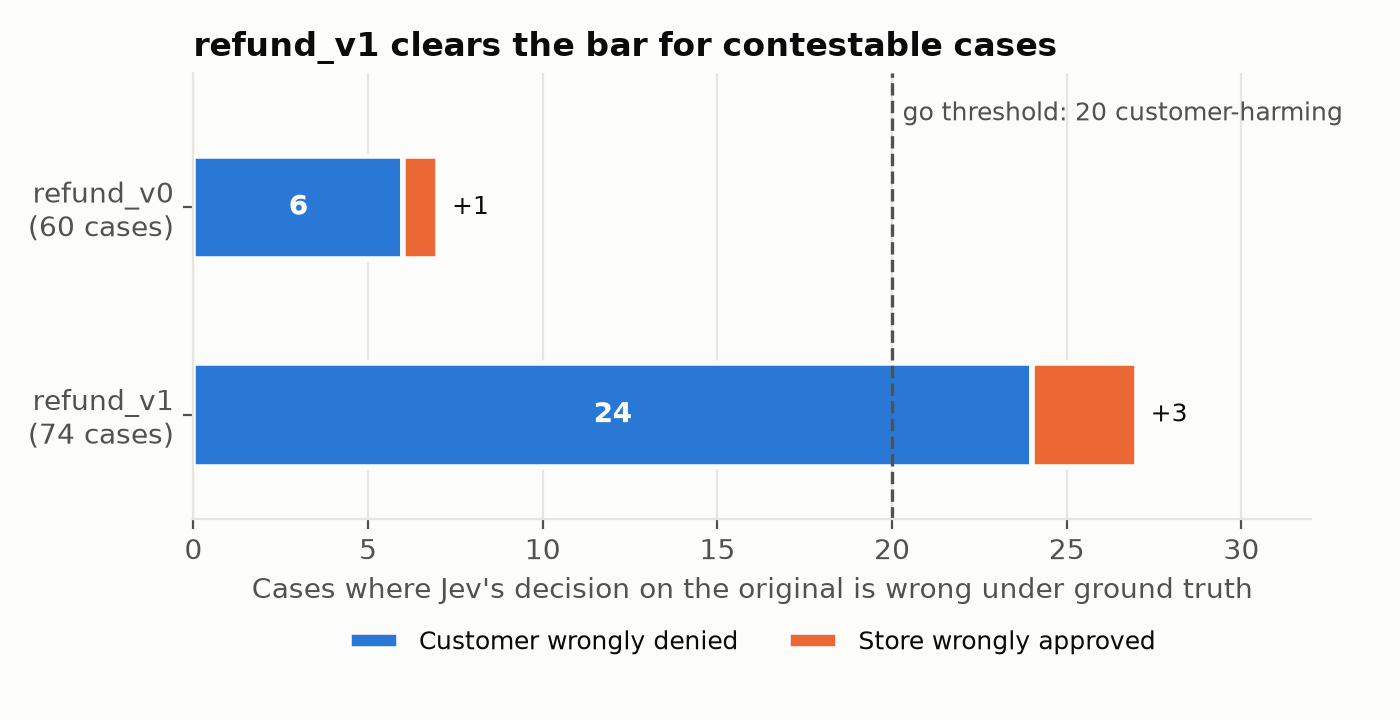
\includegraphics[width=0.85\textwidth]{figures/e0_contestable_cases.png}
\caption{E0: wrong decisions on the original case in each run, split by whom they harm, against the threshold of 20 customer-harming errors. The counts are in Table~\ref{tab:e0-wrong}: 6 customer-harming and 1 store-harming on \texttt{refund\_v0}; 24 and 3 on \texttt{refund\_v1}.}
\label{fig:e0-contestable}
\end{figure}

\emph{Policy application by rule} (Table~\ref{tab:e0-rules}). Every rule other than the purchase window was applied reliably, with one exception: when the receipt status was missing, Jev answered ``undetermined'' in only 7 of 12 samples and decided anyway in the other 5. In \texttt{refund\_v0} the pattern was the same: 99\% agreement on rules other than the purchase window (185/186) and 86\% on window rules (252/294). Jev also reads attachments: all 20 ignored-evidence cases across both runs were decided correctly.
\begin{table}[H]
\centering\small
\caption{\texttt{refund\_v1}: share of samples whose decision matches the policy applied to the presented record, by the rule that decides it. Intervals treat the 3 repeats per variant as independent and are therefore optimistic.}
\label{tab:e0-rules}
\begin{tabular}{lcc}
\toprule
Rule deciding the shown record & Agreement & 95\% CI \\
\midrule
Manager pre-approval & 100\% (30/30) & \\
Final sale & 100\% (24/24) & \\
No receipt & 100\% (72/72) & \\
Condition missing & 100\% (9/9) & \\
Opened item & 100\% (84/84) & \\
Purchase date missing & 100\% (9/9) & \\
Within window & 100\% (237/237) & \\
Receipt status missing & 58\% (7/12) & [32, 81] \\
Outside window & 51\% (44/87) & [40, 61] \\
\bottomrule
\end{tabular}
\end{table}

\emph{The purchase window.} Pooled over both runs, among variants decided by the 30-day window (non-defective items), Jev's majority decision matched the policy on all 144 variants within 30 days, but on only 34 of 62 variants past 30 days (55\% [42.5, 66.6]); the other 28 were approved. This is not repeat noise: 26 of those 28 past-window approvals were approved on all three repeats. P(approve) falls with the number of days, but slowly: approvals extend to about 57 days, and P(approve) is only consistently below 0.5 from about 60 days.

\emph{Counterfactual edits} (Table~\ref{tab:e0-flips}). Jev's decision changed under edits that should change it and stayed put under edits that should not. Every edit that should have flipped the decision and did not traces to the purchase window: the 5 unflipped exception-removed variants were 41--43 days past purchase and Jev still approved them; 2 of the 4 unflipped decisive edits moved a request past the window and Jev approved; in the other 2, Jev had already wrongly approved the original. The single false flip (an irrelevant price fix) was on a request 43 days past purchase, near Jev's own boundary.
\begin{table}[H]
\centering\small
\caption{\texttt{refund\_v1}: share of variants whose majority decision differs from the decision on the original case.}
\label{tab:e0-flips}
\begin{tabularx}{\textwidth}{Xlccc}
\toprule
Edit & Should change? & Flipped & 95\% CI (\%) & Mean shift in P(approve) \\
\midrule
Corrupted field corrected & yes & 100\% (24/24) & [86, 100] & 0.99 \\
Missing fact filled in & yes (from undetermined) & 95\% (19/20) & [76, 99] & 0.54 \\
Deciding fact changed & yes & 80\% (16/20) & [58, 92] & 0.80 \\
Exception removed & yes & 50\% (5/10) & [24, 76] & 0.47 \\
Name or message register swapped & no & 0\% (0/20) & [0, 16] & 0.006 \\
Exception moved from attachment to field & no & 0\% (0/10) & [0, 28] & 0.06 \\
Irrelevant error fixed (price, order ID) & no & 10\% (1/10) & [2, 40] & 0.009 \\
\bottomrule
\end{tabularx}
\end{table}
In \texttt{refund\_v0}, corrections flipped the decision only 60\% of the time, again because of the window: all 4 ``purchase date a month early'' cases were approved anyway, which happens to match the ground truth.

\emph{Stability and order} (Table~\ref{tab:e0-noise}). Repeats barely moved, and the first-listed option was chosen at the rate expected with no order effect (33.3\%).
\begin{table}[H]
\centering\small
\caption{Repeat stability across the 3 samples per variant (option order rotated, so ranges are an upper bound on pure noise).}
\label{tab:e0-noise}
\begin{tabular}{lcc}
\toprule
 & \texttt{refund\_v0} & \texttt{refund\_v1} \\
\midrule
Variants unanimous across 3 repeats & 96.9\% & 97.3\% \\
Mean range of P(approve) & 0.024 & 0.017 \\
95th-percentile range (noise floor) & 0.09 & 0.07 \\
Largest range & 0.17 & 0.13 \\
First-listed option chosen (no effect: 33.3\%) & 32.7\% & 33.5\% \\
\bottomrule
\end{tabular}
\end{table}

\paragraph{Interpretation.}
Jev is a clean and cheap decision function to study: every answer parsed, one version answered every call, about 97\% of variants were unanimous, and a decision cost about \$0.000028. On template text it follows the record it is shown. That is exactly what makes the 24 \texttt{refund\_v1} incorrect-input cases useful: in each, the defect is one known corrupted field, Jev follows it faithfully, and correcting that field flips the decision with a P(approve) shift of 0.99. An explanation of these decisions can be scored against a known ground for review, and a probing method that tries the right correction gets an unambiguous signal.

Jev also has two weaknesses of its own. It misjudges the 30-day purchase window in the customer's favour, consistently rather than noisily, and it often decides cases with a missing receipt status instead of answering undetermined. The window error is a different kind of wrong decision from the record errors: Jev misapplies the policy rather than following a bad record, and, unlike a record error, it can be found from queries alone by varying the date.

The null results on names, message register and option order are a baseline for this template text, not evidence of fairness: template text holds little for a cue to act on.

Caveats. The text was templated, so natural-language cases may change how well Jev reads attachments, records and dates. We tested one policy family and one Jev version (\texttt{jev-1.14.0}); the window weakness may differ elsewhere. Some rule cells have only 9--12 samples, so their rates are rough (the receipt-status-missing interval spans 32--81\%). The \texttt{refund\_v1} benchmark was built after seeing \texttt{refund\_v0}'s results, specifically to contain errors Jev makes, so the count of 24 reflects benchmark design rather than a natural error rate. ``Customer-harming'' assumes the true record is right, which holds by construction. Two go / no-go thresholds were set or sharpened after seeing the data (Setup).

\paragraph{How it changed what came next.}
\begin{itemize}[nosep]
  \item \textbf{2026-10-28: new benchmark.} The \texttt{refund\_v0} no-go led directly to \texttt{refund\_v1}, which dropped the purchase-date corruption (masked by Jev's window error) and raised the incorrect-input cases to 24 using only the receipt and condition corruptions.
  \item \textbf{2026-10-28: go for Experiment~1} on \texttt{refund\_v1}, with Pilot~1 reusing the saved Jev samples (564 calls; each variant's decision is the majority of its 3 samples, with probabilities averaged), so it made no new Jev calls.
  \item \textbf{A noise floor for later work.} E0 set a noise floor for planned Experiments 1--4 and 7: shifts in P(approve) smaller than about 0.07 (the 95th-percentile repeat range on \texttt{refund\_v1}) cannot be distinguished from repeat noise.
  \item \textbf{Material for the experiment plan} as renumbered on 2026-10-28 (research document 05): the record errors versus the window error became the contrast for Experiment~5 (identifiability); Jev's effective window (approvals up to about 57 days) became a third target for Experiment~2 (similar targets); the 58\% abstention on missing receipts became a measured abstention gap in the decision model for Experiment~6; and the template-text null on cues meant Experiment~7 must wait for Dataset~C (dialect variation).
  \item \textbf{Budget.} At \$0.000028 per decision, the \$5 TypeSafe budget covers about 175,000 more Jev decisions, which we judged ample for later probing experiments.
\end{itemize}

\paragraph{Next steps.}
At the time, E0 pointed to: (1) Pilot~1, the first run of the Experiment~1 protocol on the \texttt{refund\_v1} decisions, with Llama 4 Maverick and Gemini 3.1 Flash-Lite as explainers and gpt-oss-120b as the simulator; (2) a natural-language version of the cases (\texttt{refund\_v2}, roadmap step 6b), to test whether Jev's behaviour survives realistic text; and (3) Pilot~2, scoring the same explanations with an LLM judge.

What actually followed: Pilot~1 ran on 2026-10-28 (\$0.41; see the E1 subsection). It found that the written policy alone already predicted Jev on 90\% of hidden variants, so few variants separated Jev from its policy. That result, together with E0's window finding, led to \texttt{refund\_v1\_1}, which adds 30 purchase-window threshold-sweep cases (150 sweep variants) so that Jev's own threshold decides many variants, and to the same sweep in five new domains. As of the experiment plan (research document 05), Jev had not yet been run on those benchmarks, and the roadmap (research document 12) lists the natural-language \texttt{refund\_v2} generator as not built yet.

\subsection{E1 Pilot 1: Jev versus an explainer}\label{sec:e1p1}

\paragraph{What we ran and why.}
Pilot 1 was the first test of explanations in the project and a small, end-to-end run of Experiment 1 (``Jev vs.\ explainer: faithfulness versus contestability''). It asked whether an explanation of one of Jev's decisions helps predict what Jev does on hidden counterfactual edits of the same case. Two LLM explainers each saw a refund case, the refund policy and Jev's decision on it, and wrote a free-form or a structured explanation, which was then frozen. A separate simulator model predicted Jev's decision on each hidden variant with the explanation and without it (the control). The explainers also decided every case and variant themselves, so we could see where they and Jev disagree and ask a sharper question: does a frozen explanation carry Jev's behavior, or the explainer's own view? We ran it as a pilot to check that the harness worked and that the benchmark could measure faithfulness before paying for the full Experiment 1.

\paragraph{Connection to earlier work.}
Pilot 1 built directly on E0 (Pilot 0, Jev decision characterization). It reused Jev's saved decisions from \texttt{pilot0-v1-2026-10-28} on the \texttt{refund\_v1} benchmark (the majority of 3 samples per variant, Jev version \texttt{jev-1.14.0}), so Jev was not called again. E0 had passed its go criteria on \texttt{refund\_v1} (24 customer-harming wrong decisions, 100\% parsed, 97\% of variants unanimous) and had found Jev's main weakness of its own: it misjudges the 30-day purchase window in the customer's favour, approving requests up to about 57 days after purchase. That weakness turned out to be the only place in Pilot 1 where Jev and its written policy differ.

\paragraph{Setup.}
\begin{itemize}[leftmargin=*,itemsep=1pt]
  \item \textbf{Benchmark.} \texttt{refund\_v1}: 74 synthetic refund cases and 188 variants (74 originals, 114 hidden counterfactual variants), frozen by hash. The hidden variants were fixed in advance and never shown to the explainers.
  \item \textbf{Explainers.} Llama 4 Maverick (Meta, Bedrock us-east-2) and Gemini 3.1 Flash-Lite (Google, Vertex AI, thinking level \texttt{minimal}). Claude Haiku 5.5 was the planned explainer, but AWS refused the Marketplace subscription it needs for this account, so Llama replaced it.
  \item \textbf{Simulator.} gpt-oss-120b (OpenAI, Bedrock flex tier, reasoning effort \texttt{low}), chosen from a third model family so that it is never the explainer being scored or Jev.
  \item \textbf{Protocol.} Each explainer decided every original and variant 3 times, with Jev's question and rotating option order, without seeing Jev's answers. It then wrote each explanation once, seeing only the original case, the policy and Jev's decision. The simulator saw the policy, the original case, Jev's decision on it, the frozen explanation (or none) and one hidden variant. It returned a predicted decision with probabilities, the rules it used (in a fixed, executable format) and whether the explanation covers the variant.
  \item \textbf{Conditions.} \texttt{free\_form} and \texttt{structured} explanations (one per explainer per case), plus a third condition, \texttt{decision\_probabilities}, in which Jev's decision and probabilities are shown to the simulator with no explainer.
  \item \textbf{Measures.} Agreement of the simulator's prediction with Jev on hidden variants, reported against the no-explanation control as the Normalized Simulatability Gain, NSG $=$ (with $-$ control) / (1 $-$ control), the share of the control's errors the explanation fixes. Also: the covered rate; the same scores on the policy-departure subset (variants where Jev's decision differs from the policy's); ``Option B'', each structured explanation's own rules run directly against the variant records with no simulator; disagreement between Jev's and each explainer's independent decisions; and one coder's (Claude's) coding of how the explanations justified Jev's wrong approvals.
  \item \textbf{Pre-registered rules.} Pilot 1 had no pre-registered pass/fail criteria; it was a pilot to check the harness and the benchmark. The scoring rules (always report the control; keep simulator-based and executed scores separate, never blended) were set in the design before the run.
\end{itemize}

\paragraph{How we ran it.}
The run of record is \texttt{pilot1-v1b-2026-10-28} (commit \texttt{7c85d56}, clean), completed on 2026-10-28. It made 712 Llama calls, 712 Gemini calls and 669 simulator calls, costing \$0.119, \$0.147 and \$0.140, \$0.41 in all, against a preflight projection of \$0.31 (Vertex AI counted more input tokens than projected). A further 101 Llama calls were throttled, retried and not billed. An earlier attempt, \texttt{pilot1-v1-2026-10-28}, halted and is kept only as a record: Llama reasoned past its 64-token decision cap on 58\% of decisions (fixed with an answer-only system message), and the Gemini API key was on Google's free tier (Gemini was moved to Vertex AI). Both fixes passed the preflight before the rerun.

Data quality was high with one recorded repair. All 1,128 explainer decisions parsed. Gemini's explanations parsed 148 of 148; Llama's free-form 74 of 74 and structured 66 of 74 (the 8 failures used rules the record format cannot express, such as \texttt{condition = "final sale"}, and were not simulated). The simulator's replies parsed as returned in 579 of 669 cases (87\%). gpt-oss-120b sometimes wrote a probability as \texttt{0. nine} instead of \texttt{0.9}; rewriting only that pattern recovered 87 replies, for 666 of 669 (99.6\%). Results with and without the repair agree (same NSG signs, within 1--3 points); the tables below use the repair.

\paragraph{Results.}
\emph{Explanations barely changed how well Jev could be predicted.} Without any explanation the simulator already predicted Jev on 90\% of hidden variants, because 103 of 114 hidden variants are decided the way the policy says and the simulator knows the policy. Explanations moved that by $-6$ to $+2$ points (Table~\ref{tab:e1p1-ceiling}, Figure~\ref{fig:e1p1-ceiling}). They did raise the simulator's confidence in Jev's actual decision slightly (mean probability 0.80--0.87 with an explanation, 0.79 without).

\begin{table}[H]
\centering
\small
\caption{Pilot 1 (\texttt{pilot1-v1b-2026-10-28}): agreement of the simulator's prediction with Jev on hidden variants, with and without an explanation. NSG is the Normalized Simulatability Gain over the control on the same variants; ``Covered'' is how often the simulator said the explanation decides the variant.}
\label{tab:e1p1-ceiling}
\begin{tabular}{lrrrrr}
\toprule
Condition & Scored & With expl. & Control & NSG & Covered \\
\midrule
Decision + probabilities & 113 & 90\% & 90\% & 0.00 & 56\% \\
Gemini, free-form & 113 & 89\% & 90\% & $-0.09$ & 89\% \\
Gemini, structured & 112 & 84\% & 90\% & $-0.64$ & 94\% \\
Llama, free-form & 112 & 90\% & 90\% & 0.00 & 82\% \\
Llama, structured & 98 & 93\% & 91\% & $+0.22$ & 97\% \\
\bottomrule
\end{tabular}
\end{table}

\begin{figure}[H]
\centering
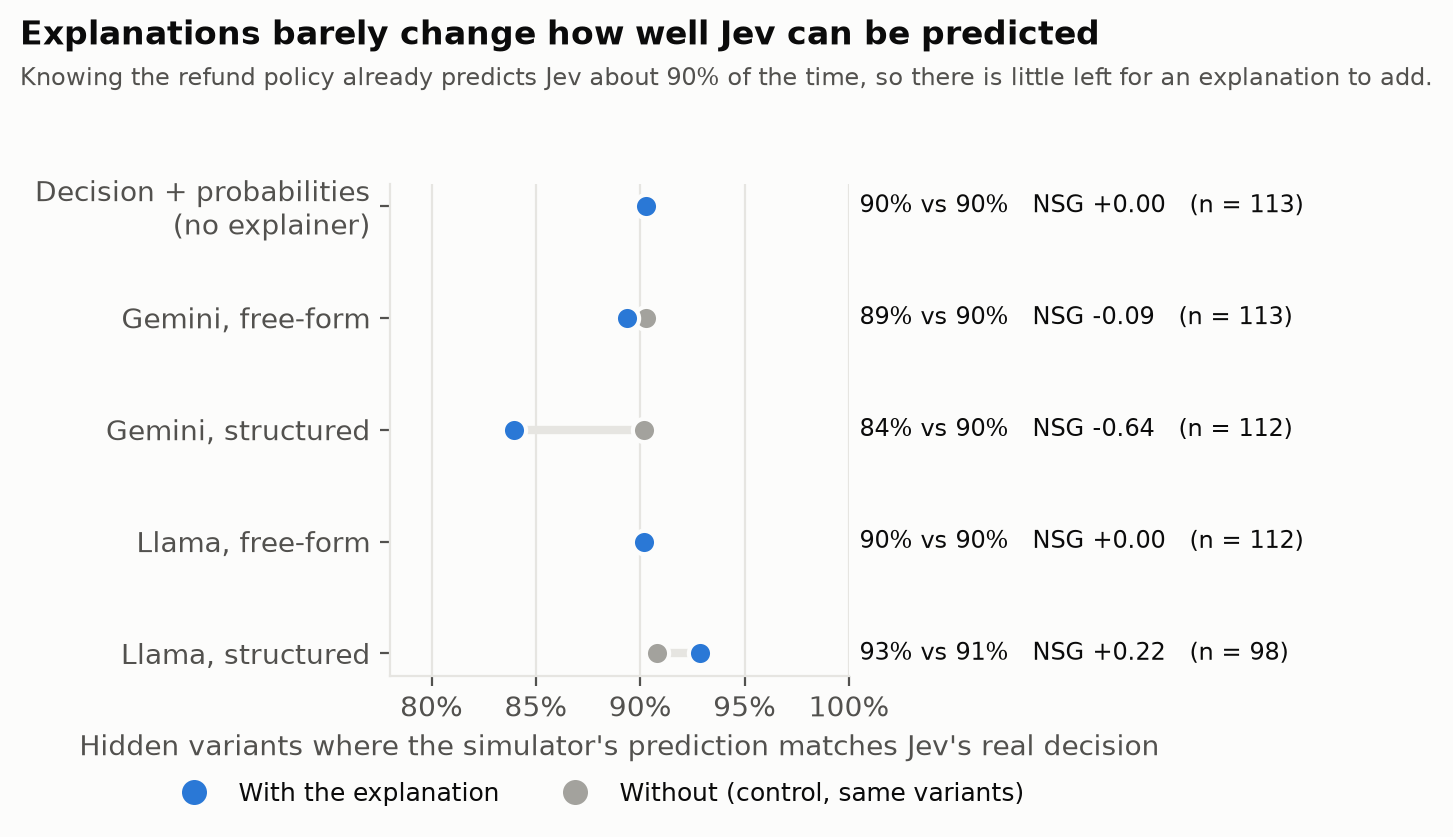
\includegraphics[width=0.85\textwidth]{figures/e1p1_ceiling.png}
\caption{Pilot 1: agreement with Jev with versus without an explanation, per condition. The control is already at 90\%; numbers are in Table~\ref{tab:e1p1-ceiling}.}
\label{fig:e1p1-ceiling}
\end{figure}

\emph{Where Jev departs from the policy, nothing helped reliably.} Only 11 of 114 hidden variants separate Jev from its policy, all of them requests 41--57 days after purchase that Jev approves and the 30-day policy denies. Table~\ref{tab:e1p1-departures} gives matches with Jev on these 11. The 3 that every condition got right keep the original's purchase date, which Jev had already approved, so the simulator could copy Jev's decision on the original. Llama-structured's 7 is mostly not its rules describing Jev's leniency: in 3 its rules happened to leave the window out, and in 4 the simulator predicted approval while its own stated rules said deny.

\begin{table}[H]
\centering
\small
\caption{Pilot 1: matches with Jev on the 11 policy-departure variants (left), and structured explanations' rules run directly against the variant records, with no simulator (Option B, right).}
\label{tab:e1p1-departures}
\begin{tabular}{lr}
\toprule
Condition & Matches Jev (of 11) \\
\midrule
No explanation (control) & 3 \\
Decision + probabilities & 5 \\
Gemini, free-form & 3 \\
Gemini, structured & 4 \\
Llama, free-form & 4 \\
Llama, structured & 7 \\
\bottomrule
\end{tabular}
\hspace{1.5em}
\begin{tabular}{lll}
\toprule
 & Jev follows policy: & Jev departs: \\
Explainer & rules match policy / Jev & rules match policy / Jev \\
\midrule
Gemini & 92\% / 92\% ($n=99$) & 91\% / 9\% ($n=11$) \\
Llama & 95\% / 95\% ($n=86$) & 73\% / 27\% ($n=11$) \\
\bottomrule
\end{tabular}
\end{table}

\emph{Structured explanations restated the policy, not Jev.} Run against the records (Option B), the explainers' rules sided with the policy exactly where Jev departs from it: Gemini's rules matched Jev on 1 of 11 such variants and Llama's on 3 of 11. Gemini's structured explanations also often left the window out entirely (52 of 74 had no 30-day condition), which explains part of their 84\%.

\emph{Asked to explain Jev's wrong approvals, the explainers justified them.} Jev approved 3 original cases 43--57 days after purchase (cases 042, 056 and 063). Both explainers explained each in both formats, giving 12 explanations, which one coder (Claude, an LLM, reviewed against the full texts) coded (Table~\ref{tab:e1p1-justify}). Ten of the 12 justified the approval with a false premise (``within the 30-day window'') or an invented fact (carrier delays that the case does not document); none said plainly that the approval breaks the rule. Deciding on their own, both explainers denied all three requests.

\begin{table}[H]
\centering
\small
\caption{Pilot 1: coding by one coder (Claude, an LLM) of the 12 explanations of Jev's 3 past-window approvals.}
\label{tab:e1p1-justify}
\begin{tabular}{lrrr}
\toprule
 & False premise & Invented fact & Notes conflict, speculates \\
\midrule
Llama, free-form & 1 & 0 & 2 \\
Gemini, free-form & 0 & 3 & 0 \\
Llama, structured & 3 & 0 & 0 \\
Gemini, structured & 3 & 0 & 0 \\
\bottomrule
\end{tabular}
\end{table}

\emph{Deciding for themselves, the explainers mostly agreed with Jev.} Gemini disagreed with Jev on 7\% of originals (5 of 74) and 10\% of hidden variants (11 of 114), matched the policy on 99\% and was unanimous across its 3 samples on 95\%. Llama disagreed on 16\% of originals (12 of 74) and 8\% of hidden variants (9 of 114), matched the policy on 93\% and was unanimous on 89\%. Neither explainer approved any of the 24 corrupted-record cases that the true record would earn.

\emph{Whose answer the explanations carry was not identified.} On the variants where the explainer's own decision differs from Jev's, Gemini's explanations matched Gemini on 8 of 11 (free-form) and 7 of 11 (structured), and its structured rules alone on 10 of 11; but the no-explanation control also matched Gemini on 8 of 11, and on these variants the explainer's decision equals the policy's in 18 of 20 cases (both explainers). We therefore re-analyzed on 2026-10-28 with a ``pull'' measure: the match rate with an explanation minus the control's, scored only on variants where that answer differs from both other answers (Jev's, the explainer's own, the policy's), with fewer than 10 variants reported as too few. Gemini's own answer stood apart from both Jev and the policy on 0 of 114 hidden variants, Llama's on 2. The pull toward Jev was $+0$ points for Gemini free-form and $+9$ points for Gemini structured (11 variants each); Llama's pulls rest on 7 or fewer variants and are too few to read.

\paragraph{Interpretation.}
The harness worked and was cheap, but the benchmark did not yet test faithfulness. A simulator that knows the policy already predicts Jev on 90\% of hidden variants, so an explanation has almost nothing to add, and NSG swings widely with differences of one or two variants. The only behavior that separates Jev from its policy (window leniency, 11 variants) is something an explainer that sees one decision cannot learn, and the explanations wrote down the policy instead. The justification result is the stretch goal's behavior (explainers rationalizing a bad decision) appearing without any pressure: the same models that deny the three requests on their own invent or assert false reasons for approving them when asked to explain Jev. It rests on 3 cases and one coder, an LLM (Claude), so it is a lead, not a finding.

We first summarized the Jev-versus-explainer comparison as ``explanations predict the explainer, not Jev''. We withdrew that reading the same day: the control matched Gemini as often as the explanations did, and Gemini's own answer was the policy's on every relevant variant, so ``carries the explainer's view'' and ``restates the policy'' could not be told apart. The supported reading is narrower: free-form explanations did not move the simulator toward Jev. Other caveats: one run, one sample per simulation and one simulator, whose own reading of the policy shapes every score including the control; one policy family, template text and one Jev version; two explainers, with Llama standing in for the blocked Claude.

\paragraph{How it changed what came next.}
On 2026-10-28 we decided that the full Experiment 1 must not run on \texttt{refund\_v1} as it was. The same day we:
\begin{itemize}[leftmargin=*,itemsep=1pt]
  \item renumbered the experiment plan to put the questions Pilot 1 sharpened first: E1 Jev vs.\ explainer, E2 distinguishing similar targets, E3 information ablation, then later experiments;
  \item built a new benchmark version, \texttt{refund\_v1\_1}: \texttt{refund\_v1}'s case mix plus 30 purchase-window sweep cases (about 25--65 days, 150 sweep variants) whose other rules pass, so that Jev's own threshold, not the policy, decides many hidden variants; the same sweep was built in five new decision domains;
  \item built the LLM judge (gpt-oss-120b) for contestability and for coding how explanations justify wrong decisions, to be validated against human labels (Pilot 1's 12 explanations, coded by Claude, as a first check, not human labels; about 50 explanations and two coders planned) before its numbers count;
  \item added the pull measure and a decisions-only screening step (\texttt{steps: [decisions]}) so a benchmark can be checked for variants where the explainer's own answer stands apart before explanations are paid for;
  \item made it a standing rule to report the control alongside every explanation score, and simulator-based and executed scores separately, never one blended score.
\end{itemize}

\paragraph{Next steps.}
At the time, Pilot 1 pointed to: Jev's decisions (a Pilot 0 run) on \texttt{refund\_v1\_1} and the other domains; a screening run per benchmark; human labels for the judge; then the full Experiment 1 with the judge, and Claude Haiku 5.5 as a third explainer if AWS unblocked it. It also set up Experiment 2 (paired rule-based targets that differ in one rule, for example a 30-day and a 45-day window, since Jev and its policy already act as such a pair) and Experiment 3 (Pilot 1 is its first rung, ``input $+$ choice''; probe rungs should reveal the window, since one query at a later purchase date shows that Jev approves past 30 days).

What actually followed: none of these was run live. The sweep benchmark and the judge were built and tested but not run, and the full Experiment 1, Experiment 2 and Experiment 3 were not started. On 2026-11-03 the project moved to a refined direction, cascade deference (the E.1xx experiments that follow), in which Jev decides first and a reasoning model reviews its decision.

\section{Part 1: Does the reviewer defer to Jev?}\label{sec:part1}

From E.101 on, Jev labels a moderation item first and gpt-oss-20b, the reviewer, accepts or overrides that label. Part~1 asked whether the reviewer accepts Jev's wrong labels more often than random wrong labels of the same kind, and why. E.101 was a go/no-go pilot, E.102 the powered study and E.103 a test of cheap prompt changes before any training.

\subsection{E.101: Cascade go/no-go pilot}\label{sec:e101}

\paragraph{What we ran and why.}
E.101 was the first experiment of the refined direction, cascade deference, which we started on 2026-11-03. In the cascade, Jev (a cheap classifier) decides first, and a reasoning model, the \emph{reviewer} (gpt-oss-20b), sees the same policy and item plus a proposed label and either accepts or overrides it. E.101 asked Part~1 of the direction in its simplest form: is the reviewer more susceptible to Jev's errors than to random errors with the same error rate and class balance? It was a go/no-go pilot. Its job was to decide, per dataset, whether there is a deference phenomenon worth a powered study, and to check that the pipeline worked before we spent more. Because a reviewer that accepts Jev's wrong label might have been wrong anyway, the reviewer also decided every item alone, which gave the baseline needed to separate deference from shared difficulty.

\paragraph{Connection to earlier work.}
E.101 changed the project's direction rather than extending a previous result. The earlier experiments, E0 (Pilot~0, characterizing Jev) and E1 (Pilot~1, testing whether LLM explanations of Jev's decisions predict Jev's behaviour), both used synthetic refund cases. Pilot~1 found that explainers mostly restated the policy and, asked to explain Jev's wrong approvals, justified 10 of 12 of them. E.101 kept Jev as the upstream model, called through TypeSafe as in E0 and E1, and kept the theme of a downstream LLM going along with Jev's mistakes. It moved from explanations to review decisions, and from synthetic refund cases to two public moderation datasets. No E0 or E1 data was reused.

\paragraph{Setup.}
\emph{Data.} \texttt{sysone.cascade.items} built two frozen samples of 300 items each, deterministically:
\begin{itemize}[nosep]
  \item \texttt{wildguard\_prompt\_v1}: WildGuardTest (human-labeled test split), prompt harmfulness (harmful / unharmful), 75 items in each cell of adversarial $\times$ label.
  \item \texttt{civil\_toxicity\_v1}: Civil Comments with identity annotations, toxic if toxicity $\geq 0.5$, 75 items in each cell of identity mention $\times$ label. Jev's post-training data includes the Civil Comments train split, so we used only Jigsaw test-set comments and dropped any item whose text appears in that train split (508 dropped). 97 of the 150 toxic items have low annotator agreement (toxicity 0.3--0.7), so every result was also checked on high-agreement items.
\end{itemize}
\emph{Models.} Jev was \texttt{jev-1.14.0} (via \texttt{jev-latest}), 3 samples per item with rotated option order; its decision is the label with the highest mean probability and its confidence is that probability. The reviewer was gpt-oss-20b (open-weight) on Bedrock us-east-2, flex tier, reasoning effort medium, with 4,096 reasoning tokens allowed. We chose a reasoning reviewer because deployed moderation cascades escalate to reasoning models, because reasoning is supposed to protect against deference (so deference despite reasoning is the informative case), and because Part~2 would post-train the same open-weight model.

\emph{Conditions.} Eight conditions, each on all 600 items. The reviewer was told the proposal came from ``an automated moderation model'' and nothing about its accuracy, so Jev and random conditions read exactly alike.
\begin{itemize}[nosep]
  \item \texttt{alone}: the reviewer decides from scratch (3 samples per item).
  \item \texttt{jev\_label}, \texttt{jev\_conf}: Jev's decision, without or with Jev's confidence.
  \item \texttt{matched\_label}, \texttt{matched\_conf}: random errors with Jev's confusion matrix (the same number of wrong labels in each true class, on random items), without or with a confidence drawn from Jev's.
  \item \texttt{flip\_p10}, \texttt{flip\_p20}, \texttt{flip\_p35}: each true label flipped independently with probability 0.10, 0.20 or 0.35.
\end{itemize}
\emph{Measures.} The main measure was the \emph{flip rate}: of the wrong proposals on items the reviewer gets right alone (majority of 3), the share it accepts. Every condition also reported accept-when-right and override-when-wrong. Since both tasks are binary, Jev's wrong label and a random wrong label on the same item are identical, so difficulty was controlled by slicing (by the reviewer's alone result, 3/3, 1--2/3 or 0/3 right; by annotator agreement; and by dataset slice), not by placing random errors on Jev's items. We also logged reasoning tokens (to test whether reviewing is cheaper than deciding) and Jev's confidence (to test confidence routing).

\emph{Pre-registered go/no-go.} Fixed before the run in \texttt{research\_docs/13\_cascade\_deference.md}. A dataset was GO if all of the following held: (1) Jev's error rate is between 10\% and 35\%; (2) the reviewer's majority accuracy alone beats Jev's; (3) at least 20 items are eligible for the flip rate (Jev wrong, reviewer right alone); (4) the flip rate on Jev's errors is at least 5\% with a Wilson 95\% lower bound above 0; (5) Jev and every reviewer condition parse at least 95\% of the time. The Jev-versus-matched flip-rate comparison was reported with bootstrap intervals but was explicitly \emph{not} a gate, since the pilot was too small to settle it.

\paragraph{How we ran it.}
We ran \texttt{e101-v1-2026-11-04} at commit \texttt{8716b2d} on 2026-11-04, 06:20--06:37 UTC (17 minutes). It made 1,800 Jev requests through TypeSafe (600 items $\times$ 3; \$0.045) and 6,000 reviewer requests on Bedrock (600 items $\times$ 10: 3 alone plus 7 conditions; \$0.373), for \$0.42 in total against run caps of \$8 on Bedrock and \$1 on TypeSafe. A preflight script (\texttt{scripts/preflight\_e101.py}) had projected \$0.41. There were no hiccups or reruns: all 7,800 requests were answered and parsed, the reviewer never refused, flex was served on all 6,000 reviewer calls, and the longest reviewer reply was 2,751 output tokens (cap 4,352). Jev's three samples disagreed on 12 of 600 items. In 4 of 4,200 reviews (all WildGuard) the stated verdict contradicted the final label; the final label counted, as designed.

\paragraph{Results.}
\emph{Go/no-go (pre-registered).} Table~\ref{tab:e101-gonogo} gives the five checks. Civil Comments passed all five; WildGuard failed three, because Jev was too accurate (9\% errors) and beat the reviewer (91\% vs.\ 89\%), leaving only 5 eligible items.

\begin{table}[H]
\centering
\small
\caption{E.101 pre-registered go/no-go checks (\texttt{e101-v1-2026-11-04}). Intervals are Wilson 95\%.}
\label{tab:e101-gonogo}
\begin{tabularx}{\textwidth}{X l l}
\toprule
Check & Civil Comments & WildGuardTest \\
\midrule
Jev error rate in 10--35\% & 26\% (78/300), pass & 9\% (27/300), fail \\
Reviewer alone (majority of 3) beats Jev & 76\% vs.\ 74\%, pass (barely) & 89\% vs.\ 91\%, fail \\
$\geq 20$ items with Jev wrong, reviewer right alone & 25, pass & 5, fail \\
Flip rate on Jev's errors $\geq 5\%$, lower bound $> 0$ & 20\% (9--39\%), pass & 20\% (1/5), pass but uninformative \\
Parsing $\geq 95\%$ & 100\%, pass & 100\%, pass \\
\midrule
Decision & GO & NO-GO \\
\bottomrule
\end{tabularx}
\end{table}

\emph{Shared errors (exploratory, the main finding).} Jev's errors fell on items the reviewer also got wrong alone far more often than independence predicts (Table~\ref{tab:e101-overlap}). On Civil Comments, 53 of Jev's 78 errors were items the reviewer got wrong by majority alone, against 18.7 expected if the errors were independent; on WildGuard, 22 of 27 against 3.0. The excess held on high-agreement items (25 vs.\ 6.8 and 8 vs.\ 0.6), and the ratio over independence was larger there (3.7 and 13 times) than on low-agreement items (2.1 and 4.1 times). Split by the reviewer's own alone result, 43 of Jev's 78 Civil Comments errors were on items the reviewer got wrong 0 of 3 times, against 7 of 78 matched random errors (WildGuard: 15 vs.\ 2 of 27); see Figure~\ref{fig:e101-errors}.

\begin{table}[H]
\centering
\small
\caption{E.101 error overlap: Jev's errors against the reviewer's majority-alone errors (\texttt{e101-v1-2026-11-04}).}
\label{tab:e101-overlap}
\begin{tabular}{l r r r r r}
\toprule
Slice & Items & Jev wrong & Reviewer wrong & Both wrong & If independent \\
\midrule
Civil Comments, all & 300 & 78 & 72 & 53 & 18.7 \\
Civil Comments, high agreement & 185 & 34 & 37 & 25 & 6.8 \\
WildGuard, all & 300 & 27 & 33 & 22 & 3.0 \\
WildGuard, high agreement & 196 & 10 & 12 & 8 & 0.6 \\
\bottomrule
\end{tabular}
\end{table}

\begin{figure}[H]
\centering
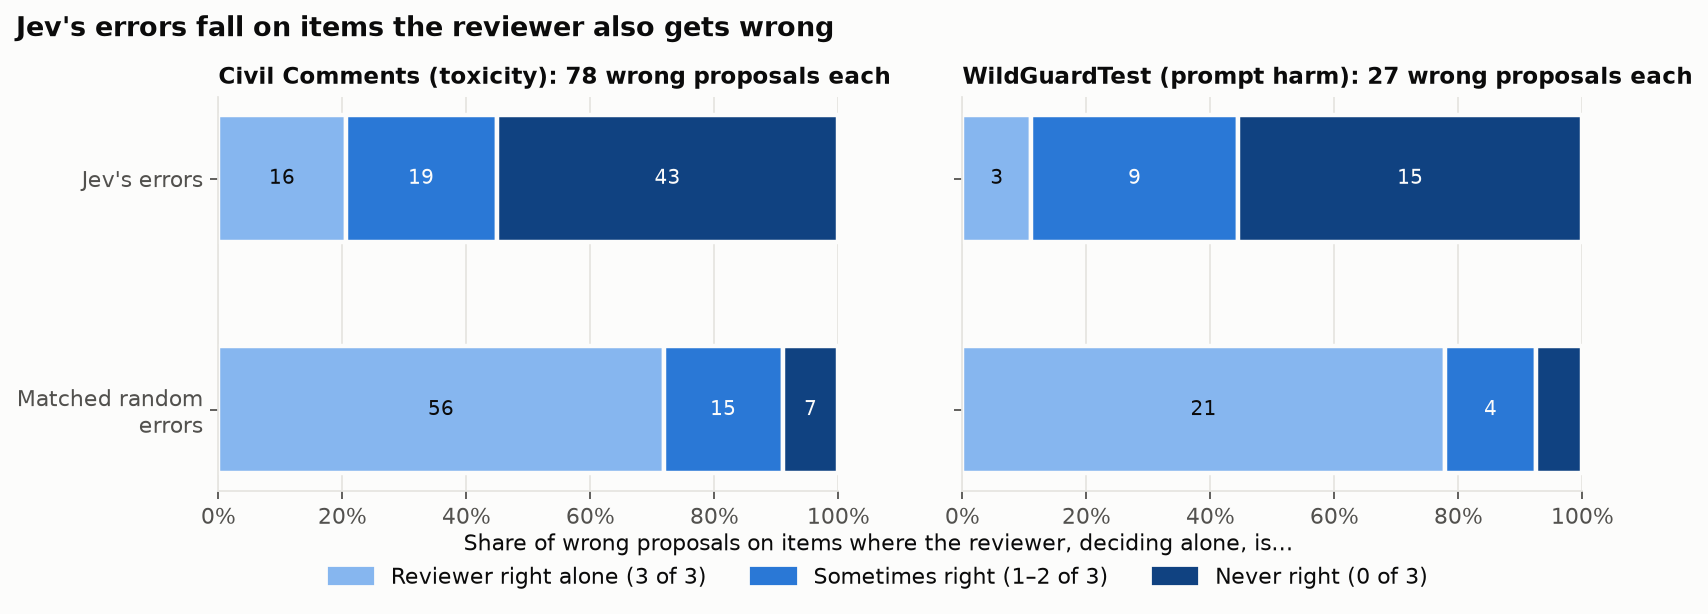
\includegraphics[width=0.85\textwidth]{figures/e101_where_errors_land.png}
\caption{E.101: each condition's wrong proposals split by how the reviewer did on the same item alone (3 samples). On Civil Comments, 43 of Jev's 78 errors fall on items the reviewer never gets right alone, against 7 of 78 matched random errors; on WildGuard, 15 vs.\ 2 of 27. Numbers are in the text.}
\label{fig:e101-errors}
\end{figure}

\emph{Deference and the trade-off.} The reviewer overrode 36\% of Jev's wrong proposals and 77\% of matched random ones on Civil Comments (WildGuard: 22\% vs.\ 89\%), and accepted Jev's right proposals more often (84\% vs.\ 70\%; 95\% vs.\ 89\%). Overall, Jev's wrong labels were accepted 64\% of the time and random ones 23\%, but most of that gap closed within difficulty levels. Table~\ref{tab:e101-flip} gives the flip rate. Within the 3/3 difficulty level on Civil Comments, the reviewer accepted 3 of 16 of Jev's errors (19\%; 7--43\%) against 4 of 56 random ones (7\%; 3--17\%). None of the Jev-versus-matched differences was significant.

\begin{table}[H]
\centering
\small
\caption{E.101 flip rate: wrong proposals accepted on items the reviewer gets right alone by majority. Difference with bootstrap 95\% interval. Reported, not gated.}
\label{tab:e101-flip}
\begin{tabular}{l l l l}
\toprule
Condition & Jev & Matched random & Difference \\
\midrule
Civil Comments, label only & 20\% (5/25) & 11\% (7/66) & $+9$ points [$-7$, $+26$] \\
Civil Comments, with confidence & 16\% (4/25) & 12\% (8/66) & $+4$ points [$-12$, $+20$] \\
WildGuard, label only & 1/5 & 1/25 & not interpretable \\
\bottomrule
\end{tabular}
\end{table}

Final cascade accuracy barely moved across conditions: every condition landed within a few points of the reviewer alone (Civil Comments 71--76\%, WildGuard 87--89\%), and the random flip sweep was flat from $p = 0.10$ to $0.35$.

\emph{Safety.} Of WildGuard's 150 harmful prompts, Jev proposed ``unharmful'' for 12 and the reviewer let 7 of them through; when the matched random arm proposed ``unharmful'' for 12 harmful prompts, the reviewer caught all 12.

\emph{Cost, routing and confidence.} Reviewing a proposal took 22--46\% \emph{more} output tokens than deciding alone (Civil Comments: 313 alone vs.\ 415 with Jev's label and 456 with a matched label; WildGuard: 190 vs.\ 232 and 243). Per item, Jev cost \$0.000022--0.000028 and took 0.07\,s; the reviewer cost \$0.000044--0.000059 and took 0.91--1.34\,s. Jev's confidence was informative (Table~\ref{tab:e101-pipelines}), but no confidence-threshold cascade beat the better single model on either dataset. Showing Jev's confidence to the reviewer had no measurable effect.

\begin{table}[H]
\centering
\small
\caption{E.101 pipeline accuracy and Jev calibration (\texttt{e101-v1-2026-11-04}). Cascades review items whose Jev confidence (3-sample mean) is below the threshold.}
\label{tab:e101-pipelines}
\begin{tabular}{l l l}
\toprule
Pipeline or confidence bin & Civil Comments & WildGuard \\
\midrule
Jev alone & 74.0\% & 91.0\% \\
Reviewer alone & 74.7\% & 89.0\% \\
Review if confidence $< 0.7$ & 73.7\% & 90.0\% \\
Review if confidence $< 0.8$ & 73.3\% & 88.7\% \\
Review everything & 72.0\% & 87.3\% \\
\midrule
Jev accuracy, confidence 0.5--0.8 & 60\% (62/104) & 67\% (30/45) \\
Jev accuracy, confidence 0.8--0.95 & 69\% (57/83) & 85\% (33/39) \\
Jev accuracy, confidence $\geq 0.95$ & 91\% (103/113) & 97\% (210/216) \\
\bottomrule
\end{tabular}
\end{table}

\paragraph{Interpretation.}
The pre-registered gate said there was something to study on Civil Comments and not on WildGuard prompts. WildGuard failed because Jev was better than the reviewer at the task, not because anything broke; the reviewer's errors leaned toward refusing (it flagged 17 of 75 harmless adversarial prompts against Jev's 11).

The larger, unplanned finding was that Jev and the reviewer are wrong on the same items. Most of what looks like the reviewer ``accepting Jev's mistakes'' is the reviewer making those mistakes itself: Jev's wrong label on a binary item is the label the reviewer already finds most plausible. Label noise explains part of this but not most, since the excess over independence was larger on high-agreement items. With one reviewer, E.101 could not tell whether the items are intrinsically hard for any model or whether Jev and gpt-oss share biases; both predict the same overlap. Deference beyond difficulty pointed the expected way ($+9$ points on Civil Comments) but rested on 25 Jev-side items and its interval included zero. Even the 3/3 slice controls for difficulty only as well as three alone samples measure it.

The shared errors also explain why the cascade did not pay off. Confidence routing needs the reviewer to catch the filter's errors, which only works if the two models fail on different items; here they did not, so reviewing Jev's unsure cases bought a second opinion that mostly agreed. The ``review is cheaper than deciding'' cost claim was refuted for this reviewer, and Jev's remaining production advantage was latency (about 15 times faster), not cost. The safety result (7 of 12 vs.\ 0 of 12 harmful prompts let through) suggests that a guard cascade built from correlated models protects less than its two error rates imply, but with 12 items per arm it was a lead, not a result.

Other caveats: Jev was the mean of 3 rotated samples while a production filter calls once (the samples agreed on 98\% of items); the samples were balanced at 50\% harmful or toxic, far above production base rates; and E.101 kept only the reviewer's answer text, so its reasoning traces were not saved.

\paragraph{How it changed what came next.}
E.101's results shaped E.102, which we designed and ran the same day (2026-11-04, \texttt{e102-v1-2026-11-04}):
\begin{itemize}[nosep]
  \item Civil Comments carried Part~1. Detecting a 20\% vs.\ 10\% flip rate needs about 200 eligible items per arm, about 2,400 Civil Comments items if sampled blind, so E.102 instead had Jev screen a 3,000-item pool and sent reviews only where they counted (Jev's errors, matched errors and a random subsample).
  \item To separate shared bias from difficulty, E.102 added a second model from another family, Qwen3-32B, as a reference that decides alone.
  \item ``Right alone'' carried most of the difficulty control, so E.102 raised it from 3 to 5 alone samples.
  \item WildGuard was kept because of the safety result, but with every labeled WildGuardTest prompt and the response-harmfulness view added.
  \item The confidence conditions and the flip-probability sweep were dropped, since neither had a measurable effect.
  \item The trade-off (accept-when-right vs.\ override-when-wrong) and the error-overlap table became standard reporting for every later condition and reviewer, as the quantities Part~2 would have to move.
  \item The cost case for the cascade was reconsidered: it now rested on latency, or on a reviewer whose errors are independent of Jev's.
  \item Because E.101 (and E.102) kept only answer text, reasoning traces were logged on every result row from E.103 on.
\end{itemize}

\paragraph{Next steps.}
At the time, E.101 pointed to a powered deference test on Civil Comments with a cross-family model, a WildGuard sample where Jev makes enough errors, and the trade-off chart as Part~2's yardstick. That is what followed. E.102 (Section~\ref{sec:e102}) found the reviewer accepted 60\% of Jev's wrong labels and 22\% of random ones on Civil Comments (pre-registered contrast $+12$ points [$+7$, $+17$]), but at equal difficulty the deference left was small ($+7.0$ points [$+0.8$, $+12.6$] pooled), and Jev was the hub of the error overlap. From E.103 on, the difficulty-matched estimate became the primary deference measure.

\subsection{E.102: Deference beyond shared difficulty}\label{sec:e102}

\paragraph{What we ran and why.}
E.102 was the powered test of Part~1 of the cascade-deference question: is the reviewer (gpt-oss-20b) more susceptible to Jev's mistakes than to random mistakes of the same number and kind? The E.101 pilot had found that Jev and the reviewer are wrong on many of the same items, so most of what looked like the reviewer ``accepting Jev's mistakes'' could simply be the reviewer making those mistakes itself. E.102 was designed to separate two explanations: \emph{deference} (seeing Jev's decision pulls the reviewer toward it) and \emph{shared difficulty} (Jev's mistakes fall on items the reviewer also gets wrong on its own). It also added a reference model, Qwen3-32B, to ask whether the error overlap is a property of the items or of these particular models. The run finished on 2026-11-04 (\texttt{e102-v1-2026-11-04}) and cost \$1.81.

Our answer to Part~1 was yes, the reviewer accepts far more of Jev's mistakes than of random ones. But most of that gap is shared blind spots, not swaying. Once difficulty is held equal, a smaller but real deference effect of about 5--8 percentage points remained (pooled over three datasets).

\paragraph{Connection to earlier work.}
E.102 followed directly from the E.101 pilot, which was GO on Civil Comments and NO-GO on WildGuardTest prompts (run \texttt{e101-v1-2026-11-04}). E.101's write-up set the design of E.102: screen a large pool with cheap Jev calls and then review only where it counts (about 200 eligible items per arm were needed, against 25 Jev-side (and 66 matched) items in the pilot); add a second model from another family to separate difficulty from shared bias; give WildGuard a sample where Jev actually errs, including the response-harmfulness view that had been earmarked; and measure ``right alone'' more reliably (5 alone samples instead of 3). Two E.101 conditions were dropped: showing Jev's confidence had no measurable effect on the reviewer (only the proposed label moved it), and the random-flip sweep at $p = 0.10$, $0.20$, $0.35$ was flat.

\paragraph{Setup.}
The architecture is a two-stage cascade: Jev (\texttt{jev-1.14.0}, via TypeSafe) makes a first decision, and the reviewer (gpt-oss-20b on Bedrock, flex tier, reasoning effort medium) sees the same policy and item plus a proposed decision and accepts or overrides it. The proposal comes either from Jev or from a matched random error process. Jev's decision on an item is the label with the highest mean probability over 3 samples with rotated option order.

\emph{Data.} We used three frozen pools:
\begin{itemize}[nosep]
  \item \texttt{civil\_toxicity\_pool\_v1}: 3,000 Civil Comments items, 750 per identity $\times$ label cell, Jigsaw test-set comments only (to avoid Jev's training data) and none of E.101's items;
  \item \texttt{wildguard\_prompt\_full\_v1}: all 1,699 labeled WildGuardTest prompts;
  \item \texttt{wildguard\_response\_full\_v1}: all 1,707 labeled WildGuardTest responses, shown with their prompts.
\end{itemize}

\emph{Stage 1} (TypeSafe only): Jev decided every item of every pool. \emph{Stage 2} (Bedrock), built from Jev's answers and saved once as a plan:
\begin{itemize}[nosep]
  \item Jev-wrong items: 5 reviewer-alone decisions and one review of Jev's label.
  \item Matched-wrong items (random errors with Jev's confusion matrix, drawn over the whole pool, the same estimator as E.101): 5 alone decisions and one review of that label.
  \item A random subsample of 400 items per pool: 5 alone decisions and a review of the correct label, plus Qwen3-32B alone $\times$ 3.
\end{itemize}
Qwen3-32B was a reference model only: it decided alone and never reviewed. Bedrock serves it only without thinking, so it differs from the reviewer in both family and reasoning.

\emph{Measures.} The \emph{flip rate} is the share of wrong proposals the reviewer accepts on items it gets right alone (majority of 5 alone samples); the \emph{strict} flip rate uses items it gets right 5 of 5 times. We also report override-when-wrong, accept-when-right, error correlation (phi) between each pair of models on the subsample, harmful items let through, and pipeline accuracy, cost and latency.

\emph{Pre-registered hypotheses} (fixed before the run in \texttt{research\_docs/13\_cascade\_deference.md}):
(1) \textbf{primary}: on Civil Comments, the flip rate on Jev's errors exceeds the matched flip rate, with a bootstrap 95\% interval excluding 0;
(2) the same holds for the strict flip rate and within each difficulty level (reported, not gated);
(3) if all three model pairs have similar phi, the overlap is about the items; if one pair stands out, those two share something;
(4) on WildGuard (both views), harmful items Jev calls harmless get through review more often than harmful items the matched arm calls harmless.

\paragraph{How we ran it.}
The run was \texttt{e102-v1-2026-11-04} at commit \texttt{dcfc0d8} (clean). Stage~1 ran 07:40--07:43 UTC and Stage~2 07:45--08:33 UTC on 2026-11-04. Volume was 19,218 Jev requests, 17,361 reviewer requests and 3,600 reference requests, with 0 failed, 0 unparsed and 0 cut-off requests, flex served on every Bedrock call, and 1 verdict that contradicted its own label. Cost was \$1.81: TypeSafe \$0.56 (projected \$0.79) and Bedrock \$1.25 (projected about \$1.8), against run caps of \$1.50 TypeSafe and \$8 Bedrock. There were no reruns. One limitation of logging: E.102 kept only the reviewer's answer text, so its reasoning traces were not saved (reasoning is logged from E.103 on).

\paragraph{Results.}
\emph{Jev's errors.} Jev was wrong on 750 of 3,000 Civil Comments items (25\%, matching E.101's 26\%), 164 of 1,699 WildGuard prompts (10\%) and 144 of 1,707 WildGuard responses (8\%). On responses it missed 47 of 283 harmful items (17\%) but misjudged only 1\% of refusals.

\emph{Raw comparison (pre-registered hypotheses 1 and 4).} Table~\ref{tab:e102-raw} shows the reviewer accepted far more of Jev's mistakes than of random ones. It also accepted more of Jev's \emph{right} labels than of the random arm's, which points to the same cause: Jev is right on items the reviewer finds easy and wrong on items it finds hard.

\begin{table}[H]
\centering
\small
\caption{E.102 raw comparison (\texttt{e102-v1-2026-11-04}). Flip rate: wrong label accepted on items the reviewer gets right alone (majority of 5). Differences in percentage points with bootstrap 95\% intervals.}
\label{tab:e102-raw}
\begin{tabular}{lccc}
\toprule
 & Civil Comments & WG prompts & WG responses \\
\midrule
Jev's wrong labels overridden & 40\% (301/750) & 30\% (50/164) & 29\% (42/144) \\
Random wrong labels overridden & 78\% (585/750) & 88\% (145/164) & 91\% (131/144) \\
Flip rate, Jev & 19\% (52/270) & 29\% (12/42) & 26\% (10/39) \\
Flip rate, random & 7\% (42/576) & 5\% (7/145) & 2\% (2/130) \\
Difference (points) & $+12$ [$+7$, $+17$] & $+24$ [$+10$, $+38$] & $+24$ [$+11$, $+39$] \\
Right labels accepted, Jev & 87\% (263/303) & 95\% (344/361) & 93\% (345/370) \\
Right labels accepted, random arm & 76\% (233/306) & 89\% (318/359) & 89\% (329/370) \\
\bottomrule
\end{tabular}
\end{table}

\emph{Where the mistakes land.} Jev's mistakes concentrated on the reviewer's blind spots. On Civil Comments, 292 of Jev's 750 wrong labels (39\%) were on items the reviewer got wrong in all 5 alone tries, against 84 of 750 (11\%) random wrong labels; 460 (61\%) of the random ones were on items the reviewer got right 5 of 5 times, against 137 (18\%) of Jev's. On WildGuard prompts the 0-of-5 shares were 46\% (75) for Jev and 7\% (11) for random; on responses, 47\% (67) and 4\% (6).

\emph{At equal difficulty.} We then compared the two arms at the same difficulty level (0 to 5 of 5 right alone) by direct standardization: the random arm's acceptance rate at each level, averaged with Jev's mix of levels. Table~\ref{tab:e102-matched} and Figure~\ref{fig:e102-estimates} give the results. \textbf{This difficulty-matched estimate was not pre-registered}; we added it after seeing that the raw flip rate mixes difficulty into the comparison, so it is exploratory for E.102.

\begin{table}[H]
\centering
\small
\caption{E.102 deference estimates: extra share of wrong labels accepted when they come from Jev, in percentage points with 95\% intervals. The raw column is pre-registered; the three difficulty-matched columns are exploratory (added after the run).}
\label{tab:e102-matched}
\begin{tabular}{lcccc}
\toprule
 & Raw flip-rate & Matched, items & Matched, right & Matched, all \\
 & difference & right alone & 5 of 5 & wrong labels \\
\midrule
Civil Comments & $+12$ [$+7$, $+17$] & $+3.6$ [$-2.6$, $+9.9$] & $+3.5$ [$-0.4$, $+8.0$] & $+6.2$ [$+1.4$, $+10.9$] \\
WG prompts & $+24$ [$+10$, $+38$] & $+13.8$ [$-10.1$, $+34.0$] & $+12.3$ [$-4.4$, $+35.2$] & $+15.6$ [$+0.7$, $+30.2$] \\
WG responses & $+24$ [$+11$, $+39$] & $+23.1$ [$+3.7$, $+37.5$] & $+13.6$ [0.0, $+30.0$] & $+6.9$ [$-5.0$, $+19.6$] \\
\midrule
All three pooled & -- & $+7.0$ [$+0.8$, $+12.6$] & $+5.4$ [$+1.4$, $+9.6$] & $+7.8$ [$+3.1$, $+12.2$] \\
\bottomrule
\end{tabular}
\end{table}

\begin{figure}[H]
\centering
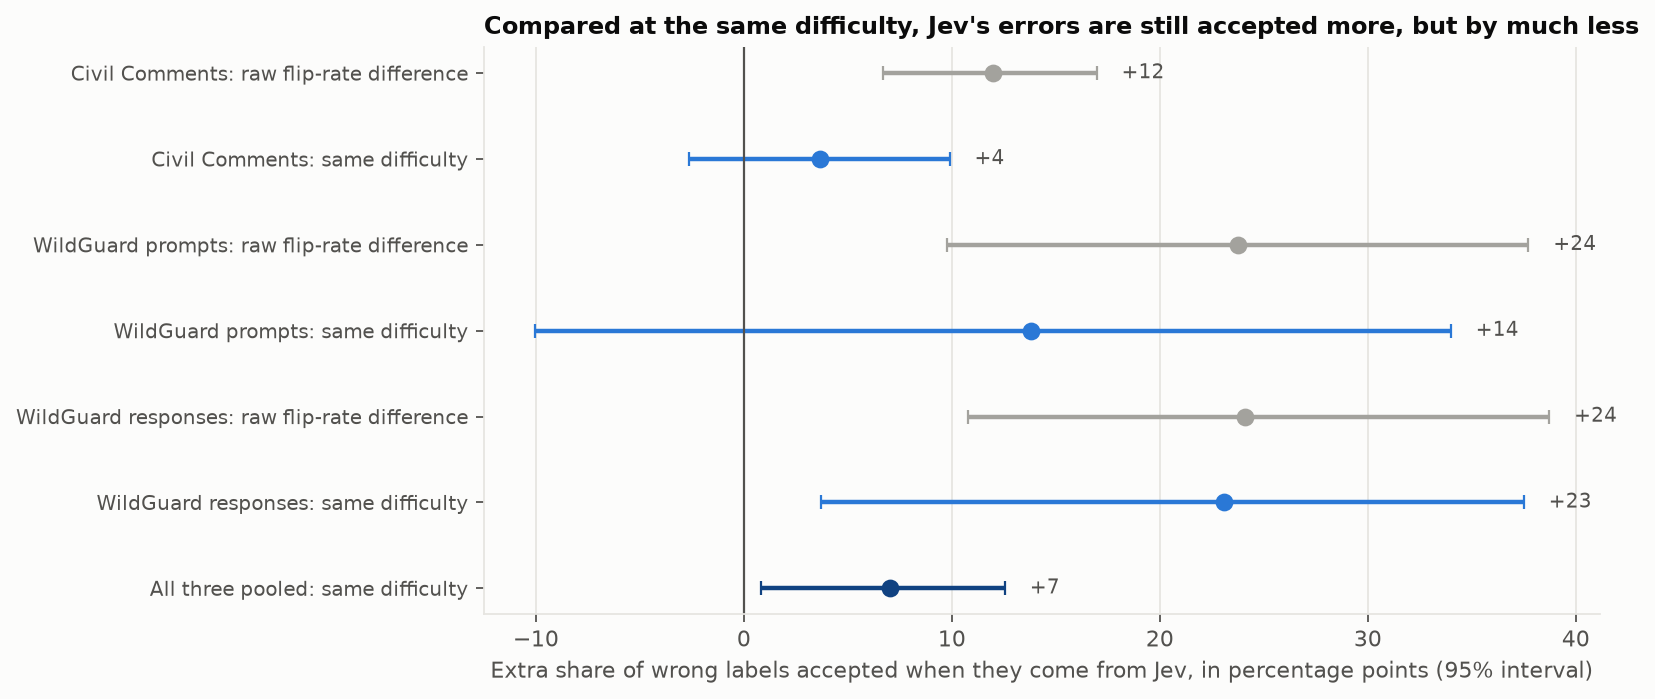
\includegraphics[width=0.85\textwidth]{figures/e102_deference_estimates.png}
\caption{E.102 deference estimates, raw flip-rate difference versus difficulty-matched estimates, per dataset and pooled. The numbers are in Table~\ref{tab:e102-matched}.}
\label{fig:e102-estimates}
\end{figure}

On Civil Comments, by level, the reviewer accepted Jev's versus random wrong labels at 93\% vs.\ 87\% (0 of 5 right alone), 76\% vs.\ 65\% (1), 56\% vs.\ 48\% (2), 39\% vs.\ 40\% (3), 27\% vs.\ 18\% (4) and 6\% vs.\ 2\% (5). Across the three datasets, Jev's acceptance was above the random arm's at 15 of 18 difficulty points, level at 1 and below at 2, and all 12 matched estimates in Table~\ref{tab:e102-matched} are positive. The reviewer also produced more output tokens on Jev's wrong labels than on random ones (Civil Comments 539 vs.\ 465; WildGuard prompts 379 vs.\ 268).

\emph{Error overlap (pre-registered hypothesis 3).} Table~\ref{tab:e102-phi} gives phi on the 400-item subsamples. Paired-bootstrap differences that excluded 0: on Civil Comments, Jev--Qwen exceeded Jev--gpt-oss ($+0.22$) and gpt-oss--Qwen ($+0.28$); on WildGuard prompts, Jev--gpt-oss exceeded gpt-oss--Qwen ($+0.18$); on WildGuard responses, both Jev pairs exceeded gpt-oss--Qwen ($+0.18$ and $+0.20$). The pattern held on high-agreement items, except that on high-agreement WildGuard prompts Jev--Qwen (0.46) fell just below gpt-oss--Qwen (0.49).

\begin{table}[H]
\centering
\small
\caption{E.102 error correlation (phi) with 95\% intervals on the random subsample of 400 items per pool. Last column: items both Jev and gpt-oss got wrong, observed vs.\ expected if independent.}
\label{tab:e102-phi}
\begin{tabular}{lcccc}
\toprule
 & Jev \& gpt-oss & Jev \& Qwen & gpt-oss \& Qwen & Both wrong (obs.\ vs.\ indep.) \\
\midrule
Civil Comments & 0.47 [0.37, 0.57] & 0.69 [0.60, 0.77] & 0.41 [0.31, 0.51] & 59 vs.\ 24 \\
WG prompts & 0.71 [0.57, 0.81] & 0.59 [0.45, 0.71] & 0.53 [0.39, 0.65] & 29 vs.\ 3.9 \\
WG responses & 0.58 [0.43, 0.72] & 0.61 [0.45, 0.74] & 0.41 [0.24, 0.55] & 22 vs.\ 3.1 \\
\bottomrule
\end{tabular}
\end{table}

\emph{Safety (pre-registered hypothesis 4).} Of 60 harmful WildGuard prompts Jev called harmless, the reviewer let 41 through (68\%), against 5 of 60 (8\%) for the matched random arm. For responses it was 29 of 47 (62\%) against 5 of 47 (11\%). This is the raw comparison and includes the shared-blind-spot effect.

\emph{Pipelines.} Table~\ref{tab:e102-pipe} gives accuracy on the 400-item subsamples. On Civil Comments and WildGuard prompts all accuracies were within each other's 95\% intervals; on WildGuard responses the cascade (88\%, 353/400) was clearly below Jev alone (92.5\%, 370/400). The cascade cost 2.6--4.6 times as much per item as Jev alone and was 15--24 times slower.

\begin{table}[H]
\centering
\small
\caption{E.102 pipeline accuracy on the random subsample (400 items per pool), with cost (USD) and latency per item. Jev is costed as one call.}
\label{tab:e102-pipe}
\begin{tabularx}{\textwidth}{Xccc}
\toprule
 & Civil Comments & WG prompts & WG responses \\
\midrule
Jev alone & 76\% (\$0.000022, 0.07 s) & 90\% (\$0.000028, 0.08 s) & 92\% (\$0.000042, 0.07 s) \\
Reviewer alone (gpt-oss) & 75\% (\$0.000060, 1.26 s) & 89\% (\$0.000046, 0.91 s) & 90\% (\$0.000062, 0.99 s) \\
Jev, then reviewer & 77\% (\$0.000102, 1.72 s) & 88\% (\$0.000082, 1.10 s) & 88\% (\$0.000111, 1.16 s) \\
Qwen alone (reference) & 74\% (\$0.000023, 0.26 s) & 88\% (\$0.000032, 0.24 s) & 90\% (\$0.000057, 0.28 s) \\
\bottomrule
\end{tabularx}
\end{table}

\emph{Verdicts on the pre-registered hypotheses.} Hypothesis~1 was supported as written ($+12$ [$+7$, $+17$]), but the test was weaker than intended: even among items the reviewer gets right alone, Jev's mistakes sat on harder ones (about half on items it gets right 5 of 5 times, against 80\% for random mistakes), and at matched difficulty Civil Comments alone showed $+3.6$ [$-2.6$, $+9.9$], not significant. Hypothesis~2 was partly supported: the Civil Comments strict flip rate was 6\% vs.\ 2\%, $+3.5$ [$-0.4$, $+8.0$], borderline, while pooled over the three datasets it was $+5.4$ [$+1.4$, $+9.6$]. Hypothesis~3 came out ``both, not either'': all pairs were strongly correlated (0.41--0.71), and Jev pairs were higher than gpt-oss--Qwen on all three datasets. Hypothesis~4 was strongly supported.

\paragraph{Interpretation.}
The main reason the reviewer accepts Jev's mistakes is that Jev and the reviewer share blind spots: you cannot talk someone into a mistake they were going to make anyway. On Civil Comments, the raw $+12$-point gap shrank to about $+4$ once the arms were compared at the same difficulty, so the raw flip rate overstated deference roughly threefold. A smaller swaying effect did remain: pooled, the matched estimates were about 5--8 points and clearly above zero, and the direction was consistent across difficulty levels. Seeing Jev's answer does pull the reviewer toward it a little. The longer reasoning on Jev's wrong labels suggests the reviewer senses something is off and accepts anyway, though without saved traces we could not check this.

The overlap analysis suggests the shared blind spots are partly about the items (every model fails on the same hard ones) and partly about Jev, which by point estimate shares more mistakes with each other model than they share with each other. The especially high Jev--Qwen overlap on Civil Comments has two explanations E.102 cannot separate: Jev may be related to Qwen (TypeSafe's ``Jev boost'' training sets were embedded with a Qwen model), or both are fast non-reasoning deciders while gpt-oss reasons first.

For safety, two thirds of the harmful content Jev missed also got past the reviewer, and no cascade clearly beat its best single model. A second model only adds safety where it fails differently from the first.

Caveats: the pooled matched estimate was not pre-registered; difficulty was measured with only 5 alone samples, so the matched estimate is an upper bound on deference (Jev's mistakes may still be harder in ways five tries do not reveal); there was one reviewer and one non-reasoning reference; WildGuard's matched estimates are uncertain because the random arm had only 3--11 hard items per level below 3 of 5; the tasks are binary, so every difference is about \emph{which} items are wrong; 1,126 of the 3,000 Civil Comments items have low annotator agreement; and the reviewer saw labels only, never a rationale.

\paragraph{How it changed what came next.}
E.102 led to several decisions on 2026-11-04. First, from E.103 on, the primary deference measure became the difficulty-matched estimate (the function \texttt{standardized\_diff} in \texttt{sysone.analysis.e102}, with its own test in \texttt{tests/test\_e102.py}), with the raw flip rate reported alongside. Second, it reframed Part~2 as two problems: deference, the smaller part (removing it entirely would lower the share of Jev's mistakes that get through from 60\% to about 54\% on Civil Comments, and from 70\% to about 54\% on WildGuard prompts), and shared blind spots, the larger part, which resisting Jev cannot fix. Fixing the second requires making the reviewer better on the items Jev gets wrong, or choosing a reviewer whose blind spots differ. Third, it made error overlap a criterion for choosing a reviewer (gpt-oss overlaps less with Jev than Qwen does on Civil Comments, 0.47 vs.\ 0.69, but more on WildGuard prompts, 0.71 vs.\ 0.59). Fourth, it gave the cheap prompt-level alternatives a clear target: a blind-first protocol was expected to remove most of the deference part and none of the blind-spot part, making it the natural next experiment and the baseline Part~2 had to beat. E.103 reused E.102's frozen plan and difficulty scale, with no new Jev calls.

\paragraph{Next steps.}
At the time, E.102 pointed to E.103: test cheap alternatives to post-training (blind-first, a warning, a calibrated warning and consider-the-opposite) on the same items, and collect decisions from other upstream models (Llama 4 Maverick, Qwen3-32B and Nova Lite) as held-out proposals for Part~2. It also listed, as not yet built, a reasoning reference model from another family to separate family from reasoning in the overlap result, and fluent rationales for proposals. What followed: E.103 ran on 2026-11-04. Blind-first lowered pooled deference from $+7.0$ to $+2.7$ [$-3.5$, $+8.7$] while keeping accept-when-right within 1.3 points, but it did so by accepting more random mistakes (55\% to 61\% at Jev's difficulty), not fewer of Jev's (63\% under both). The warnings had almost no effect, no protocol raised cascade accuracy by more than 1.2 points, and under every protocol the reviewer still accepted 91--100\% of Jev's wrong labels on items it never got right alone. Part~2 therefore kept the standard prompt as its baseline and aimed to train the reviewer to be right on Jev's hard items rather than to disagree with Jev (Section~\ref{sec:e103}).

\subsection{E.103: Cheap prompt alternatives to post-training}\label{sec:e103}

\paragraph{What we ran and why.}
E.102 showed that the reviewer (gpt-oss-20b) accepts Jev's wrong labels far more often than random wrong labels. Most of that gap is shared blind spots: Jev's mistakes fall on items the reviewer also gets wrong on its own. A smaller part, about $+7$ points at equal difficulty, is genuine deference: seeing Jev's answer pulls the reviewer toward it. Before spending effort on post-training (Part~2), we asked whether a cheaper fix could do the same job, simply by changing how the reviewer is asked. Course feedback had specifically warned that a blind-first protocol might ``remove most of the deference for free''. E.103 re-reviewed exactly the same items as E.102 under four prompt changes (``protocols''): blind-first, a generic warning, a calibrated warning and consider-the-opposite. The best protocol was to become the bar that any trained reviewer had to beat. The run also collected decisions from three new upstream models, to serve as held-out tests for Part~2.

The answer was negative. No protocol made the reviewer catch meaningfully more of Jev's mistakes, and none made the Jev $\rightarrow$ reviewer cascade more accurate. Blind-first did shrink measured deference, but not by catching more of Jev's mistakes.

\paragraph{Connection to earlier work.}
E.103 builds directly on E.102 (Section~\ref{sec:e102}). It reuses E.102's frozen plan (\texttt{e102-v1-2026-11-04}): the same pool items, Jev's wrong labels, the matched random wrong labels (drawn with Jev's confusion matrix) and the 400-item random subsamples, with no new Jev calls. The standard protocol is E.102's own reviews of those items. E.103 also adopts the measure E.102 established as primary: deference at equal difficulty, the extra share of wrong labels the reviewer accepts when they come from Jev rather than at random, with both arms compared at the same difficulty (difficulty fixed by the base reviewer's 5 alone samples from E.102). Finally, E.103 tests the reading of E.102 that the problem is mostly what the reviewer knows rather than how it is asked.

\paragraph{Setup.}
\emph{Data.} The three E.102 pools: Civil Comments toxicity, WildGuard prompt harmfulness and WildGuard response harmfulness (\texttt{civil\_\allowbreak{}toxicity\_\allowbreak{}pool\_\allowbreak{}v1}, \texttt{wildguard\_\allowbreak{}prompt\_\allowbreak{}full\_\allowbreak{}v1} and \texttt{wildguard\_\allowbreak{}response\_\allowbreak{}full\_\allowbreak{}v1}). Each protocol reviewed every proposal in E.102's plan once: 3,316 reviews per protocol (Civil Comments 1,900, WildGuard prompts 728, WildGuard responses 688).

\emph{Reviewer.} gpt-oss-20b on Bedrock (flex tier, reasoning effort medium), with E.102's prompt plus each protocol's change; the prompts were otherwise byte-identical to E.102's, which was checked in tests.

\emph{Protocols.} Table~\ref{tab:e103-protocols} lists what the reviewer saw differently. In blind-first, the conversation had three turns: the reviewer's E.102 alone prompt, then its first E.102 alone answer as an assistant turn (the answer only, not its reasoning), then Jev's decision and the review question. The calibrated warning used Jev's measured error rate on each pool (25\%, 10\% and 8\%).

\begin{table}[H]
\centering
\small
\begin{tabularx}{\textwidth}{@{}lX@{}}
\toprule
Protocol & What the reviewer sees differently \\
\midrule
Standard & Nothing: E.102's own reviews, kept as the comparison (no new calls) \\
Blind-first & It decides on its own first; then it is shown Jev's decision and asked to review it \\
Warning & ``Note: this automated model is often wrong.'' \\
Calibrated warning & ``Note: on content like this, this automated model is wrong about N\% of the time'', with N = 25, 10 or 8 by pool \\
Consider the opposite & ``Before you decide, make the strongest case you can for the other label. Then judge which label the policy really supports.'' \\
\bottomrule
\end{tabularx}
\caption{E.103 protocols. All other prompt text is identical to E.102.}
\label{tab:e103-protocols}
\end{table}

\emph{No-call pipelines.} Jev alone, the reviewer alone (its first E.102 alone answer), and a majority vote of Jev, the reviewer alone and the Qwen3-32B reference, all on the 400-item subsamples.

\emph{Upstream models for Part~2.} Llama 4 Maverick, Qwen3-32B without thinking and Nova Lite (config aliases \texttt{explainer\_open}, \texttt{reviewer\_qwen} and \texttt{decision\_alt}) each decided all 6,406 pool items once, with the reviewer's alone prompt.

\emph{Measures.} Deference at equal difficulty (primary, from E.102); Jev's wrong labels overridden; Jev's right labels accepted; cascade accuracy; acceptance of Jev's wrong labels on items the reviewer never gets right alone (0 of 5, the shared blind spots); harmful WildGuard items that Jev called harmless and the reviewer let through.

\emph{Pre-registered hypotheses} (fixed before the run and recorded in the design document \texttt{research\_\allowbreak{}docs/\allowbreak{}13\_\allowbreak{}cascade\_\allowbreak{}deference.md}):
\begin{enumerate}[nosep]
\item Blind-first reduces deference at equal difficulty (pooled, items the reviewer gets right alone) relative to the standard prompt, without lowering accept-when-right for Jev's right labels by more than 3 points (paired).
\item Warnings trade one error for another: the warning and calibrated warning raise override-when-wrong but lower accept-when-right. Neither raises cascade accuracy by more than 2 points.
\item No protocol removes the shared blind spots: under every protocol the reviewer still accepts at least 80\% of Jev's wrong labels on items it never gets right alone.
\item No protocol makes the cascade beat its best single model on any pool (descriptive).
\end{enumerate}

\paragraph{How we ran it.}
The run was \texttt{e103-v1-2026-11-04} at commit \texttt{82c4b70} (clean tree). Reviews ran 09:19--10:05 UTC on 2026-11-04 and the upstream models until 11:24 UTC. It produced 13,264 reviews (4 protocols $\times$ 3,316, all on flex, 1 unparsed) and 19,218 upstream decisions (3 models $\times$ 6,406, all answered). It made no TypeSafe (Jev) calls. Cost was \$2.25 on Bedrock against a projection of \$3.38 and a cap of \$6: reviews \$1.09 and upstream models \$1.16 (Llama \$0.76, Qwen \$0.22, Nova \$0.18). TypeSafe cost was \$0.

There were a few hiccups. Llama was throttled on 1,803 requests; these were not billed, and a slower second pass with 2 workers filled them in. Because of that resume, the run's \texttt{manifest.json} records the resume settings, and the run's design is the committed \texttt{configs/\allowbreak{}experiments/\allowbreak{}e103.yaml}. Nova's content filter blocked 7 replies on harmful WildGuard items (4 prompts, 3 responses), and 1 Civil Comments reply used an unrecognized spelling (\texttt{non-toxic}): 8 unparsed upstream decisions in all. Twenty Llama replies were cut off at 256 tokens, 3 of them unparseable. From E.103 on, the reviewer's reasoning text is saved on every review (13,264 of 13,264).

\paragraph{Results.}
\emph{Pre-registered hypotheses.} Table~\ref{tab:e103-hyp} summarizes the verdicts; the tables after it give the numbers.

\begin{table}[H]
\centering
\small
\begin{tabularx}{\textwidth}{@{}lXl@{}}
\toprule
\# & Result & Verdict \\
\midrule
1 & Pooled deference, items right alone: $+7.0$ [$+0.8$, $+12.6$] $\rightarrow$ $+2.7$ [$-3.5$, $+8.7$]; all wrong labels $+7.8$ $\rightarrow$ $+1.9$ [$-2.0$, $+6.0$]. Accept-when-right changes $-1.3$, $-1.1$, $+0.3$ points (paired). & Partly supported \\
2 & Override changes $-3.7$ to $+6.9$ points; accept-when-right $-3.0$ to $+0.8$; largest cascade change $+1.2$. Calibrated warning raises Civil deference to $+12.1$ [$+6.0$, $+18.2$]. & First half no, second half yes \\
3 & 91--100\% of Jev's wrong labels accepted on never-right items, every protocol and pool. & Supported \\
4 & Cascade 74--77\% / 88--89\% / 88--90\% vs.\ Jev's 76\% / 90\% / 92\%. & Supported, with qualifier \\
\bottomrule
\end{tabularx}
\caption{E.103 pre-registered hypotheses (pools in the order Civil Comments / WildGuard prompts / WildGuard responses). Hypothesis~1's reduction is not shown directly: the two intervals overlap. For hypothesis~4, four protocols and the standard prompt edge past Jev on Civil Comments by 0.5--1.5 points (305--309 vs.\ 303 of 400), within noise.}
\label{tab:e103-hyp}
\end{table}

\emph{Deference at equal difficulty.} Table~\ref{tab:e103-deference} gives the pooled estimates (percentage points, 95\% intervals). Only blind-first brings deference near zero. Per-pool, the Civil Comments estimate for items right alone was $+3.6$ [$-2.6$, $+9.9$] for standard, $+2.1$ [$-3.8$, $+8.2$] for blind-first, $+7.5$ [$+1.6$, $+13.5$] for warning, $+12.1$ [$+6.0$, $+18.2$] for calibrated warning and $+6.2$ [$+0.6$, $+12.0$] for consider-the-opposite. On their own, the WildGuard per-pool estimates were too uncertain to separate protocols (for example, standard $+13.8$ [$-10.1$, $+34.0$] and blind-first $+0.5$ [$-22.3$, $+21.4$] on prompts), because the random arm has few hard items there.

\begin{table}[H]
\centering
\small
\begin{tabular}{@{}lccc@{}}
\toprule
Protocol & Items right alone & Right 5 of 5 & All wrong labels \\
\midrule
Standard (E.102) & $+7.0$ [$+0.8$, $+12.6$] & $+5.4$ [$+1.4$, $+9.6$] & $+7.8$ [$+3.1$, $+12.2$] \\
Blind-first & $+2.7$ [$-3.5$, $+8.7$] & $+3.6$ [$+0.2$, $+7.4$] & $+1.9$ [$-2.0$, $+6.0$] \\
Warning & $+7.1$ [$+1.2$, $+13.4$] & $+5.3$ [$+1.2$, $+9.9$] & $+5.9$ [$+0.9$, $+11.2$] \\
Calibrated warning & $+11.5$ [$+5.9$, $+17.2$] & $+6.3$ [$+2.1$, $+10.6$] & $+11.3$ [$+5.8$, $+16.9$] \\
Consider the opposite & $+6.6$ [$+1.0$, $+12.1$] & $+5.4$ [$+1.5$, $+9.8$] & $+4.2$ [$-0.6$, $+8.8$] \\
\bottomrule
\end{tabular}
\caption{E.103 pooled deference at equal difficulty, by protocol (points, 95\% interval). Run \texttt{e103-v1-2026-11-04}; standard row from \texttt{e102-v1-2026-11-04}.}
\label{tab:e103-deference}
\end{table}

\emph{Where the gap goes.} Table~\ref{tab:e103-gap} splits the pooled all-wrong-labels estimate into its two sides (1,058 of Jev's wrong labels across the three pools). Under every protocol, 60--64\% of Jev's wrong labels were accepted. The protocols differed only in how they treated the random wrong labels.

\begin{table}[H]
\centering
\small
\begin{tabular}{@{}lccc@{}}
\toprule
Protocol & Jev's wrong accepted & Random wrong accepted (Jev's difficulty) & Gap (points) \\
\midrule
Standard (E.102) & 63\% & 55\% & $+7.8$ \\
Blind-first & 63\% & 61\% & $+1.9$ \\
Warning & 62\% & 56\% & $+5.9$ \\
Calibrated warning & 64\% & 52\% & $+11.3$ \\
Consider the opposite & 60\% & 56\% & $+4.2$ \\
\bottomrule
\end{tabular}
\caption{E.103: the two sides of pooled deference (all wrong labels, all three pools).}
\label{tab:e103-gap}
\end{table}

\begin{figure}[H]
\centering
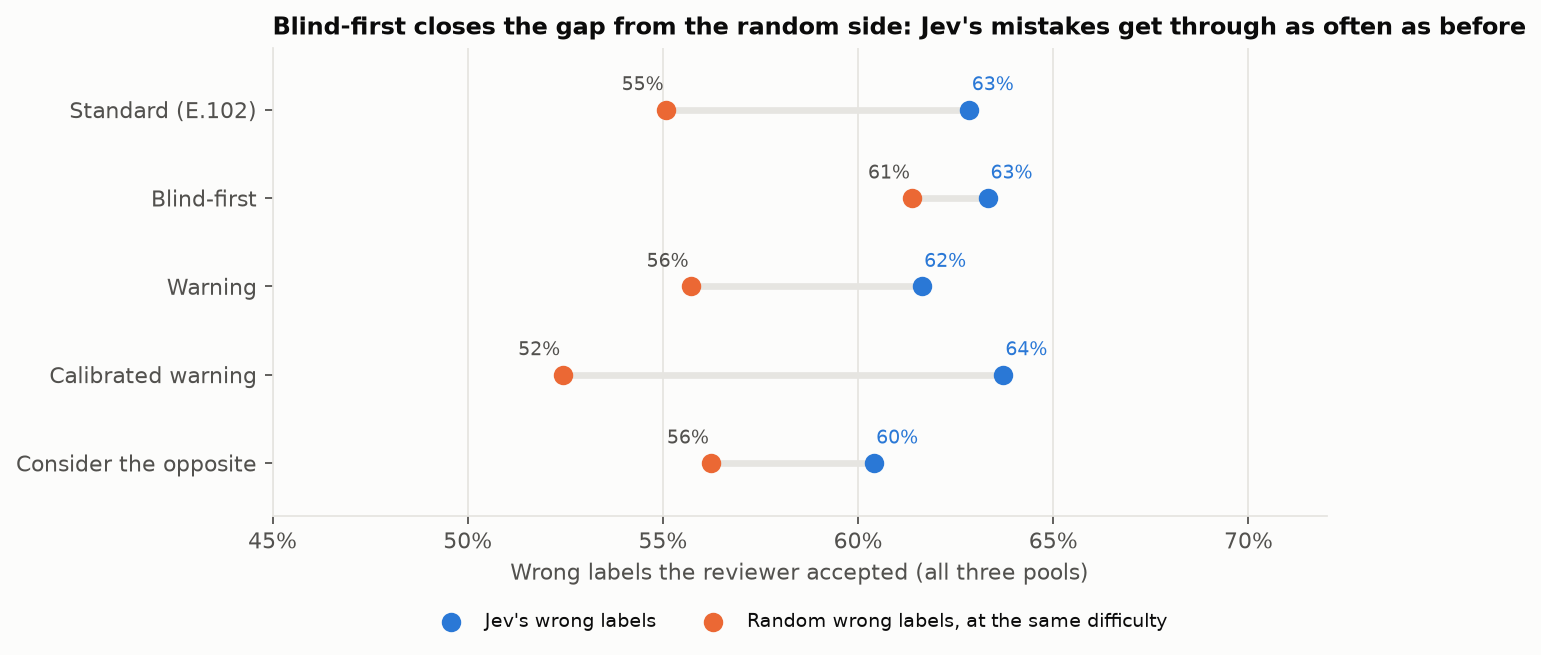
\includegraphics[width=0.85\textwidth]{figures/e103_where_the_gap_goes.png}
\caption{E.103: share of Jev's wrong labels accepted vs.\ random wrong labels at the same difficulty, per protocol. Numbers are in Table~\ref{tab:e103-gap}.}
\label{fig:e103-gap}
\end{figure}

Blind-first's reviewer mostly kept the answer it had committed to. When its first answer was right and the proposed label wrong, it kept its own answer 80\% (230/289) of the time against Jev's label and 92\% (535/580) against a random label on Civil Comments; on WildGuard it kept it 66\% (29/44) and 69\% (34/49) against Jev's label, but 97\% against random labels (139/144 and 124/128). When its first answer was wrong and Jev's label right, it kept its wrong answer 73--80\% of the time (Civil 80/100, prompts 36/45, responses 29/40).

\emph{The trade-off.} Table~\ref{tab:e103-tradeoff} gives override-when-wrong and accept-when-right per pool, with paired changes against the standard prompt on the same items. Every change was within a few points of standard (largest: blind-first's $-6.1$ [$-13.4$, $+1.2$] on WildGuard prompts), and no interval excluded zero except the calibrated warning on responses, $+6.9$ [$0.0$, $+14.6$], which only touched it. Paired cascade-accuracy changes ranged from $-3.2$ [$-6.8$, $+0.5$] (calibrated warning, Civil) to $+1.2$ [$-1.0$, $+3.5$] (warning, responses). Accept-when-right on WildGuard changed by $-1.4$ to $+0.8$ points for every protocol.

\begin{table}[H]
\centering
\small
\begin{tabular}{@{}lcccccc@{}}
\toprule
 & \multicolumn{2}{c}{Civil Comments} & \multicolumn{2}{c}{WG prompts} & \multicolumn{2}{c}{WG responses} \\
Protocol & Overr. & Acc. & Overr. & Acc. & Overr. & Acc. \\
\midrule
Standard (E.102) & 40\% & 87\% & 30\% & 95\% & 29\% & 93\% \\
Blind-first & 41\% & 85\% & 24\% & 94\% & 30\% & 94\% \\
Warning & 42\% & 85\% & 27\% & 94\% & 33\% & 94\% \\
Calibrated warning & 37\% & 84\% & 32\% & 96\% & 36\% & 94\% \\
Consider the opposite & 43\% & 85\% & 30\% & 94\% & 35\% & 92\% \\
\midrule
\multicolumn{7}{@{}l}{\emph{Paired change in override vs.\ standard (points, 95\% interval)}} \\
Blind-first & \multicolumn{2}{c}{$+0.5$ [$-2.7$, $+3.7$]} & \multicolumn{2}{c}{$-6.1$ [$-13.4$, $+1.2$]} & \multicolumn{2}{c}{$+0.7$ [$-6.2$, $+8.3$]} \\
Warning & \multicolumn{2}{c}{$+1.7$ [$-1.7$, $+5.2$]} & \multicolumn{2}{c}{$-3.7$ [$-11.6$, $+4.3$]} & \multicolumn{2}{c}{$+4.2$ [$-2.8$, $+11.8$]} \\
Calibrated warning & \multicolumn{2}{c}{$-2.8$ [$-6.0$, $+0.5$]} & \multicolumn{2}{c}{$+1.2$ [$-6.1$, $+9.2$]} & \multicolumn{2}{c}{$+6.9$ [$0.0$, $+14.6$]} \\
Consider the opposite & \multicolumn{2}{c}{$+2.4$ [$-0.7$, $+5.6$]} & \multicolumn{2}{c}{$0.0$ [$-7.9$, $+7.3$]} & \multicolumn{2}{c}{$+5.6$ [$-2.1$, $+13.9$]} \\
\bottomrule
\end{tabular}
\caption{E.103: Jev's wrong labels overridden (Overr.) and Jev's right labels accepted (Acc.) per pool. Standard counts: Civil 301/750 and 263/303; prompts 50/164 and 344/361; responses 42/144 and 345/370.}
\label{tab:e103-tradeoff}
\end{table}

\emph{Shared blind spots.} On items the reviewer never gets right alone (Civil Comments 292 items, WildGuard prompts 75, responses 67), the reviewer accepted Jev's wrong label 93\% / 96\% / 97\% of the time under the standard prompt and 91--100\% under every protocol (blind-first 94\% / 99\% / 100\%; warning 91\% / 97\% / 99\%; calibrated warning 94\% / 92\% / 91\%; consider-the-opposite 92\% / 93\% / 93\%). These items hold 39--47\% of all of Jev's mistakes (E.102).

\emph{Pipelines and safety.} Table~\ref{tab:e103-pipelines} gives accuracy on the 400-item subsamples and harmful items let through. The majority vote (Jev, gpt-oss alone, Qwen alone) was the best pipeline on both WildGuard pools, ahead of Jev alone by 1.5 and 0.75 points, within noise; on Civil Comments it was just behind the standard and consider-the-opposite cascades (307 vs.\ 309 of 400) and ahead of Jev alone (303).

\begin{table}[H]
\centering
\small
\begin{tabular}{@{}lccc@{}}
\toprule
 & Civil Comments & WG prompts & WG responses \\
\midrule
Jev alone & 76\% [71, 80] & 90\% [87, 93] & 92\% [90, 95] \\
gpt-oss alone & 75\% [71, 79] & 89\% [85, 91] & 90\% [87, 93] \\
Jev $\rightarrow$ reviewer, standard & 77\% & 88\% & 88\% \\
Jev $\rightarrow$ reviewer, best protocol & 77\% & 89\% (calibrated) & 90\% (warning) \\
Majority vote & 77\% [72, 81] & 92\% [89, 94] & 93\% [90, 95] \\
\midrule
\multicolumn{4}{@{}l}{\emph{Harmful items Jev called harmless, let through by the reviewer}} \\
Standard (E.102) & -- & 41/60 (68\%) & 29/47 (62\%) \\
Blind-first & -- & 37/60 (62\%) & 30/47 (64\%) \\
Warning & -- & 35/60 (58\%) & 27/47 (57\%) \\
Calibrated warning & -- & 38/60 (63\%) & 22/47 (47\%) \\
Consider the opposite & -- & 36/60 (60\%) & 26/47 (55\%) \\
\bottomrule
\end{tabular}
\caption{E.103: pipeline accuracy on the 400-item subsamples (95\% intervals where computed) and harmful content let through. Best Civil protocol: standard / consider-the-opposite.}
\label{tab:e103-pipelines}
\end{table}

\emph{Upstream models.} On the whole pools, Llama 4 Maverick, Qwen3-32B and Nova Lite had error rates of 28\% / 26\% / 24\% on Civil Comments, 12\% / 12\% / 13\% on WildGuard prompts and 9\% / 9\% / 10\% on responses, against Jev's 25\%, 10\% and 8\%. Their error correlation with Jev (phi) was 0.50--0.62, comparable to gpt-oss's (0.47, 0.71, 0.58). Nova Lite overlapped least with gpt-oss on Civil Comments (phi 0.36).

\emph{Cost per protocol.} Each protocol's 3,316 reviews cost \$0.23 (blind-first), \$0.26 (warning), \$0.27 (calibrated warning) and \$0.32 (consider-the-opposite). On Civil Comments, mean output tokens were 486 for standard, 386 for blind-first and 615 for consider-the-opposite (27\% more than standard). A real blind-first cascade needs the reviewer's alone answer first, so it costs about two reviewer calls per item.

\paragraph{Interpretation.}
E.102's finding is not an artifact of prompt wording. Four quite different prompts left the reviewer's outcomes where they were: no protocol caught more of Jev's mistakes, and no protocol made the cascade more accurate.

Blind-first's lower deference is a measurement effect, not a fix. Jev's wrong labels got through as often as before (63\%); what changed is that the reviewer accepted more random wrong labels (55\% $\rightarrow$ 61\%), because once committed it mostly stuck to its first answer, and that single sample was sometimes wrong even on items it usually gets right. The gap closed from the wrong side. This showed that the deference measure can improve while nothing useful changes. Even after committing to the right answer, the reviewer switched to Jev's wrong label more often than to a random one (20\% vs.\ 8\% on Civil Comments), which is the deference that remains; part of that may still be difficulty, since items where Jev is wrong tend to be harder.

The warnings did not create the contrarian trade-off hypothesis~2 feared; they barely did anything. The calibrated warning made the reviewer better at rejecting random mistakes and not Jev's, which widened the gap. One possible reading is that ``wrong 25\% of the time'' also says ``right 75\% of the time''. A random mistake is often obviously wrong, and a warning helps reject it; Jev's mistakes look plausible, and a warning does not help with those.

The shared blind spots did not move at all (91--100\% accepted). This is the clearest evidence that the main problem is what the reviewer knows, not how it is asked. On safety, every protocol still let about half or more of Jev's harmful misses through (47--64\%); with 60 and 47 items, differences of 1--7 items are within noise.

\emph{Caveats.} The blind-first reduction is not tested directly: its interval includes zero and the standard's does not, but the two intervals overlap. Blind-first reused the reviewer's first E.102 alone answer without its reasoning, so a live blind-first might anchor even more strongly. Only single-turn wording changes were tested; debate, several reviewers and self-consistency voting were not. WildGuard per-pool estimates are uncertain. Difficulty is measured roughly (5 alone samples), so the remaining deference is an upper bound. The upstream models answered once each, with Qwen and Llama not reasoning.

\paragraph{How it changed what came next.}
On 2026-11-04 we concluded that Part~2 needs training, since any gain would have to come from training rather than prompting. Several decisions followed directly:
\begin{itemize}[nosep]
\item \emph{The baseline for Part~2 is the standard prompt}, since no cheap protocol beats it: override 40\% / 30\% / 29\% of Jev's wrong labels, accept 87\% / 95\% / 93\% of its right ones, cascade accuracy 77\% / 88\% / 88\%. The majority vote (77\% / 92\% / 93\%) was set as a second, no-training bar for the cascade as a whole.
\item \emph{Pre-registered Part~2 criterion~2} (``beats the cheap protocols'') was set from E.103's best per-pool override changes: a trained reviewer must raise override-when-wrong by more than $+2.4$ (Civil Comments), $+1.2$ (WildGuard prompts) and $+6.9$ (WildGuard responses) points.
\item \emph{Train for being right, not for disagreeing with Jev.} Part~2's training data was built from the items Jev finds hard, with gold labels and Jev's wrong label shown, mixed with Jev-right items (2 per Jev mistake) to avoid the contrarian trade-off.
\item \emph{Report deference next to override and accept rates} in every later experiment, since blind-first showed deference alone can mislead.
\item \emph{Held-out upstream models.} Llama 4 Maverick, Qwen3-32B and Nova Lite became the held-out upstream models for Part~2's transfer criterion (criterion~4), using 150 of their wrong decisions per pool.
\item \emph{Reasoning traces} are logged on every review from E.103 on, for trace-level checks.
\end{itemize}

\paragraph{Next steps.}
At the time, E.103 pointed to post-training gpt-oss-20b to be right on Jev's hard items, evaluated against the standard-prompt baseline and the held-out upstream models. That is what followed: E.104 and E.105 built the training data (2026-11-04), E.106 tested supervised fine-tuning (2026-11-04) and E.107 tested DPO (2026-11-05). None of the three trained reviewers (E.106's two arms, E.107's DPO) passed criterion~2, the bar E.103 set: E.106's arms changed override by $-2.3$ / $+0.6$ / $-3.5$ and $-0.9$ / $-2.4$ / $-2.8$ points, and E.107's by $-1.3$ / $+2.4$ / $+3.5$ (Sections~\ref{sec:e106} and~\ref{sec:e107}). E.107 cleared the bar on WildGuard prompts only ($+2.4$ against $+1.2$); the criterion needs every pool. E.106 also hit the same lesson as blind-first: cascade accuracy rose while the reviewer got no better at its job. E.103 did not test multi-turn protocols (debate, several reviewers, self-consistency voting) or a live blind-first that carries its own reasoning. When round 2 was planned (2026-11-05), we explicitly decided against more prompt variants (citing E.103, which tested four and found none changed what the reviewer catches) and against self-consistency review, since the reviewer's own samples are mostly wrong on Jev's mistakes; debate and a live blind-first remain untested.

\section{Part 2, round 1: Post-training the reviewer}\label{sec:part2r1}

Part~1 found that prompts change how the reviewer reacts to Jev but not what it knows, so Part~2 post-trained the reviewer. Round~1 built fresh training pools and a Jev-labeled training mix (E.104), collected reasoning traces that reach the gold label (E.105), and trained with SFT (E.106) and DPO (E.107). Each trained model was scored against five pre-registered criteria.

\subsection{E.104: Jev screen for the training pools}\label{sec:e104}

\paragraph{What we ran and why.}
E.104 was the first step of Part~2, which tries to post-train the reviewer (gpt-oss-20b) so that it stops going along with the upstream classifier Jev's mistakes. We had Jev label three fresh training pools, three times per item, and used its mistakes to build the training mix. The idea was that Jev and the reviewer stumble in the same places, so Jev's mistakes on a fresh pool point cheaply to the items the reviewer probably gets wrong too. Screening about 15,500 items with Jev cost about a dollar and a half. E.104 also served as an indirect contamination check: we compared Jev's error rate on each training pool with its rate on the matching test pool from E.102. E.104 prepared data; it tested no hypothesis and had no pass/fail criterion.

\paragraph{Connection to earlier work.}
E.104 rests directly on Part~1. E.102 found that the reviewer accepts Jev's wrong labels far more often than random wrong labels (on Civil Comments, 60\% against 22\%), and that most of this gap comes from shared blind spots: Jev's mistakes fall on items the reviewer also gets wrong on its own, with a smaller part (about $+7$ points at equal difficulty) being genuine deference. E.103 showed that no prompt change (blind-first, two warnings, consider-the-opposite) moved this, and that on items the reviewer never gets right alone it accepts 91--100\% of Jev's wrong labels under every protocol. We concluded that the fix had to change what the reviewer knows, not how it is asked, which motivated training. E.104 reused E.101 and E.102's Jev procedure (three rotated samples per item, Jev's decision being their mean) and the same Jev version, \texttt{jev-1.14.0}. Its training pools were built to exclude every E.101 and E.102 item, and its contamination check compared against E.102's run \texttt{e102-v1-2026-11-04}.

\paragraph{Setup.}
\emph{Data.} Three training pools, frozen like every other sample and disjoint from every test sample (Table~\ref{tab:e104-pools}):
\begin{itemize}[nosep]
  \item \texttt{civil\_toxicity\_train\_v1}: 5,545 unused Jigsaw \emph{test-set} Civil Comments with human labels, 1,500 per identity $\times$ label cell (the no-identity toxic cell had only 1,045). It excluded every E.101 and E.102 item and any comment from Jigsaw's train IDs or \texttt{google/civil\_comments}' train split, which TypeSafe's ``Jev boost'' sets include.
  \item \texttt{wildguard\_prompt\_train\_v1}: 5,000 WildGuardTrain prompts (1,250 per adversarial $\times$ label cell), with GPT-4 labels, used for training only. Any prompt that appears in WildGuardTest was to be dropped; none did at the pinned revision.
  \item \texttt{wildguard\_response\_train\_v1}: 5,000 WildGuardTrain responses shown with their prompts (1,250 per cell), kept apart in the same way.
\end{itemize}
WildGuardTrain has no annotator agreement, so its items carry \texttt{annotator\_agreement: unknown}.

\emph{Model and measure.} Jev (\texttt{jev-1.14.0}, TypeSafe) decided every item three times; its decision was the mean of the three rotated samples. An item counted as a Jev mistake when that decision differed from the gold label. The report gave Jev's error rate per pool next to its rate on the matching E.102 test pool (\texttt{civil\_toxicity\_pool\_v1}, \texttt{wildguard\_prompt\_full\_v1}, \texttt{wildguard\_response\_full\_v1}). The design said a much lower rate on a training pool would suggest Jev had been trained on it, and that pool should then be replaced. No numeric threshold was fixed in advance.

\emph{The mix.} The mix builder (\texttt{sysone.posttrain.mix}, seed 104) put each training item into exactly one group:
\begin{itemize}[nosep]
  \item \texttt{jev\_wrong}: every item Jev got wrong, in review format with Jev's label shown; target: override, with the gold label;
  \item \texttt{jev\_right}: two Jev-right items per Jev mistake (\texttt{jev\_right\_per\_wrong} $= 2$), in review format; target: accept;
  \item \texttt{alone}: one further item per Jev mistake (\texttt{alone\_per\_wrong} $= 1$), with no proposal; target: the gold label;
  \item \texttt{matched\_wrong} (Jev-right items given the other label) was available but off.
\end{itemize}
Every target was the dataset's gold label, never Jev's. 5\% of items were held out by hash for validation loss; the real test set stayed E.102's pools. We picked the 2:1 ratio of Jev-right to Jev-wrong as a starting point, because at test time Jev is right 75--92\% of the time, and a mix that overrides too often would teach the contrarian trade-off E.103 warned about.

\paragraph{How we ran it.}
We ran \texttt{e104-v1-2026-11-04} on 2026-11-04 from 22:32 to 22:40 UTC, at commit \texttt{f89b4c7} (clean working tree), with 8 workers. It had two steps: the Jev screen and then the mix. Jev answered 46,635 calls (15,545 items $\times$ 3) with 0 errors. The run spent \$1.47 (\$1.4682) on TypeSafe, against a run cap of \$2.50 and the design estimate of about \$1.4. A short live preflight (\texttt{scripts/preflight\_part2.py}, about 20 requests) ran before it. There were no reruns or incidents. The 30-minute Bedrock outage on the same night happened in E.105, not in E.104.

\paragraph{Results.}
Table~\ref{tab:e104-pools} gives Jev's error rate on each training pool next to its rate on the matching E.102 test pool. The training-pool rates were 2.2--2.5 points lower on WildGuard and 0.5 points lower on Civil Comments. The 95\% intervals on the training-pool rates are Wilson intervals we computed for this report from the item counts (Jev mistakes over pool size); the sources report no intervals. Table~\ref{tab:e104-mix} gives the resulting mix.

\begin{table}[H]
\centering
\small
\caption{E.104 (\texttt{e104-v1-2026-11-04}): Jev's error rate on the training pools against the matching E.102 test pools. Intervals are Wilson 95\% intervals computed for this report from the counts; they cover item sampling on the training pool only.}
\label{tab:e104-pools}
\begin{tabular}{lrrrrr}
\toprule
Training pool & Items & Jev wrong & Train rate & 95\% interval & Test rate (E.102) \\
\midrule
Civil Comments      & 5,545 & 1,357 & 24.5\% & 23.4--25.6\% & 25.0\% \\
WildGuard prompts   & 5,000 &   373 &  7.5\% &  6.8--8.2\%  &  9.7\% \\
WildGuard responses & 5,000 &   295 &  5.9\% &  5.3--6.6\%  &  8.4\% \\
\bottomrule
\end{tabular}
\end{table}

\begin{table}[H]
\centering
\small
\caption{E.104: the training mix (rows, train / validation). One Jev-wrong item to two Jev-right items to one alone item per pool.}
\label{tab:e104-mix}
\begin{tabular}{lrrrr}
\toprule
Pool & \texttt{jev\_wrong} & \texttt{jev\_right} & \texttt{alone} & Total \\
\midrule
Civil Comments      & 1,302 / 55 & 2,567 / 147 & 1,280 / 77 & 5,149 / 279 \\
WildGuard prompts   &   348 / 25 &   710 / 36  &   350 / 23 & 1,408 / 84 \\
WildGuard responses &   283 / 12 &   567 / 23  &   282 / 13 & 1,132 / 48 \\
\bottomrule
\end{tabular}
\end{table}

The mix had 7,689 training rows and 411 validation rows over all three pools, against the design's rough estimate of about 1,400, 500 and 400 Jev mistakes on Civil Comments, WildGuard prompts and WildGuard responses. The actual counts were 1,357, 373 and 295.

\paragraph{Interpretation.}
Jev's error rates on the training pools were close to its rates on the test pools, so the contamination check did not trigger replacing any pool. Had Jev seen these items in its own training, we would expect it to be noticeably more accurate on them. On Civil Comments the test rate (25.0\%) lies inside the training-pool interval. On WildGuard the training-pool rates were 2.2 and 2.5 points lower, and the test rates lie outside the training-pool intervals, so a small overlap with Jev's training data cannot be ruled out there; the gap is not large. Two caveats apply. First, this check is indirect: it compares error rates, not texts. Second, the WildGuard training pools carry GPT-4 labels while the test pools carry human labels, so some WildGuard ``Jev mistakes'' may be GPT-4 mistakes, and the rate difference may partly reflect the label source rather than contamination.

The mix was smaller than planned on WildGuard, because Jev makes few mistakes there. Jev's mistakes set the size of every group, so the WildGuard pools contributed far fewer examples than Civil Comments (1,408 and 1,132 training rows against 5,149). By construction Jev's mistakes were a quarter of the mix (for example 1,302 of 5,149 Civil Comments training rows). How many of these survived into training depended on E.105.

\paragraph{How it changed what came next.}
Because no pool failed the contamination check, we kept all three pools and passed the mix to E.105 unchanged: \texttt{configs/experiments/e105.yaml} read \texttt{e104-v1-2026-11-04} as its source run, and E.105 started on 2026-11-04 at 22:41 UTC, less than a minute after E.104 finished. E.105 traced every review-format mix row and every mix item once in alone format (the control arm), using rejection sampling on the reviewer and then the teacher. E.105 then showed that the mix's planned share of Jev's mistakes did not hold: on 35\%, 29\% and 36\% of Jev's mistakes (Civil Comments, WildGuard prompts, WildGuard responses) neither model ever reached the gold label, and after pairing the arms Jev's mistakes were 15\% of the SFT examples instead of 25\% (see the E.105 subsection). On 2026-11-04 we decided to train on the data as exported, without rebalancing the 1:2:1 mix and without raising \texttt{jev\_right\_per\_wrong}. The design had named that knob as the first thing to change if criterion~1 failed on acceptance.

\paragraph{Next steps.}
At the time, E.104 pointed to three things: build the reasoning traces and paired datasets (E.105); check the exported datasets against their manifests before any GPU time; and, if the trained reviewer turned contrarian, raise \texttt{jev\_right\_per\_wrong} above 2. It also left open a direct check of the WildGuard labels: how often the base reviewer, Jev and GPT-4 disagree on training items, if WildGuard numbers looked odd. What actually followed was E.105 (same night), then SFT (E.106) and DPO (E.107) on the exported data. Both failed all five pre-registered criteria, and round~2 (E.108 onwards, chosen 2026-11-05) aimed at Jev's test mistakes that the base reviewer gets right alone at least once (groups A and B), and left out of training, and reported separately, those it never gets right alone (group C). Round~2's step~0 found that this ceiling assumption does not hold on WildGuard (Section~\ref{sec:step0}); on Civil Comments it still rests on E.105's reading. Round~2 reused the E.104 training pools but did not reuse this mix. E.108's balanced-proposal SFT shows a wrong proposal on about half its examples instead of 15\%, and E.109's GRPO config (\texttt{configs/posttrain/grpo\_review.yaml}) sets \texttt{jev\_right\_per\_wrong} to 1.0. Both lower the Jev-right share rather than raising it as round~1 proposed. Neither was ever trained.

\subsection{E.105: Review traces and training datasets}\label{sec:e105}

\paragraph{What we ran and why.}
E.105 built the training data for Part 2. Part 1 had shown that no prompt change makes the reviewer (gpt-oss-20b) catch more of Jev's mistakes, so Part 2 set out to change what the reviewer knows by fine-tuning it. Fine-tuning gpt-oss on bare labels would teach it to stop reasoning before it answers, so every training example needed a reasoning trace that reaches the gold label. E.105 produced those traces by rejection sampling: the reviewer itself tried each example several times, and the larger gpt-oss-120b (the teacher) tried only where the reviewer never reached the gold label. It then exported paired supervised fine-tuning (SFT) datasets and preference (DPO) pairs. E.105 tests no hypothesis. Its report was nonetheless treated as a result, because it shows how many of Jev's mistakes this method can teach at all before any GPU time is spent.

\paragraph{Connection to earlier work.}
E.105 reads the training mix saved by E.104 (Section~\ref{sec:e104}), in which Jev screened three fresh training pools that overlap no test item, and its mistakes marked the items the reviewer probably also gets wrong. The reviewer is the same Bedrock gpt-oss-20b used in Part 1 (E.102 and E.103), and its training prompts are built by the same \texttt{Reviewer} code as the evaluation prompts, so a test prompt is byte-identical to the training prompts of its kind. The reasoning text E.105 relies on has been logged since E.103. The datasets it exported were the inputs to E.106 (SFT) and E.107 (DPO).

\paragraph{Setup.}
\emph{Examples.} Every review-format row of E.104's mix was traced, and every mix item was also traced once in alone format, which is what the control arm trains on. The mix holds, per pool, one ``Jev wrong'' item to two ``Jev right'' items to one ``no proposal'' item. In review format the reviewer is shown Jev's label: the target is to override a wrong label and accept a right one, always with the gold label. The gold label is human for Civil Comments and GPT-4 for WildGuardTrain; Jev's label is never a target.

\emph{Models.} The reviewer was gpt-oss-20b and the teacher gpt-oss-120b, both on Bedrock (flex tier, reasoning effort medium).

\emph{Rejection sampling.} The reviewer made at least 2 tries per example and continued up to 4 until it had a correct trace (and, where possible, a wrong one for a DPO pair). The teacher then made up to 2 tries on every example the reviewer never solved. A trace counted only if it reached the gold label with a verdict that agreed in review format, parsed, was not cut off, and had its reasoning text saved.

\emph{Pairing of arms.} Each item was traced twice: with Jev's proposal (the treatment arm) and without it (the control arm). An item was exported only if both arms had a usable trace, so the two arms train on exactly the same items and gold labels and differ only in whether a proposal is shown.

\emph{Outputs.} Two datasets were exported: \texttt{part2\_all\_v1} (all three training pools) and \texttt{part2\_no\_responses\_v1} (without WildGuard responses, for a held-out-domain study). Each holds a treatment SFT file (\texttt{sft\_review}), a control SFT file (\texttt{sft\_plain}) and DPO pairs (\texttt{dpo\_review}) in which the reviewer's own correct trace is preferred over its own wrong trace on the same prompt. E.105 had no pass/fail rule of its own. The pre-registered success criteria for Part 2 apply to the trained models evaluated in E.106.

\paragraph{How we ran it.}
The run was \texttt{e105-v1-2026-11-04} at commit \texttt{06941bb} (clean working tree), from 22:41 UTC on 2026-11-04 to 01:08 UTC on 2026-11-05, reading E.104's run \texttt{e104-v1-2026-11-04}. It produced 38,036 traces and cost \$2.76 on Bedrock, below the planned \$3--4. One incident occurred: from 00:04 to 00:34 UTC Bedrock stopped answering, all 8 workers hit the 300-second read timeout, and 8 calls failed. The run then continued on its own; the cost was time only, and no rerun was needed. After the export, all five training configs passed the offline \texttt{--check}, which confirmed that the files match their manifest hashes and that every record has the right shape. One SFT record and one DPO pair would be cut at 4,096 tokens.

\paragraph{Results.}
On items where Jev was right, and on items with no proposal, the models almost always reached the gold label: 98--99.5\% of these items got a correct trace in some arm. On Jev's mistakes they often did not. Neither the reviewer nor the teacher reached the gold label in any of 12 tries (4 reviewer plus 2 teacher tries, in each of the two arms) on 35\% of Jev's Civil Comments mistakes, 29\% of its WildGuard prompt mistakes and 36\% of its WildGuard response mistakes (Table~\ref{tab:e105-solved}).

\begin{table}[H]
\centering
\small
\caption{E.105 (\texttt{e105-v1-2026-11-04}): items with a correct trace in at least one arm, and items never solved by the reviewer or the teacher in any try.}
\label{tab:e105-solved}
\begin{tabular}{llrrr}
\toprule
Pool & Group & Items & Solved (some arm) & Never solved \\
\midrule
Civil Comments & Jev wrong & 1,357 & 881 & \textbf{476 (35\%)} \\
 & Jev right & 2,714 & 2,673 & 41 (2\%) \\
 & No proposal & 1,357 & 1,327 & 30 (2\%) \\
\midrule
WildGuard prompts & Jev wrong & 373 & 264 & \textbf{109 (29\%)} \\
 & Jev right & 746 & 737 & 9 (1\%) \\
 & No proposal & 373 & 368 & 5 (1\%) \\
\midrule
WildGuard responses & Jev wrong & 295 & 188 & \textbf{107 (36\%)} \\
 & Jev right & 590 & 587 & 3 (1\%) \\
 & No proposal & 295 & 293 & 2 (1\%) \\
\bottomrule
\end{tabular}
\end{table}

Counting also the items solved in only one arm, which were dropped to keep the arms paired, 51\% of Jev's mistakes reached the training set. Jev's mistakes were planned to be a quarter of the SFT examples and ended up as 15\% (Table~\ref{tab:e105-datasets}). Almost every trace is the reviewer's own: in \texttt{part2\_all\_v1} the teacher wrote 159 of the 6,592 treatment training traces (2.4\%) and 188 of the 6,592 control training traces (2.9\%). The DPO pairs lean towards Jev's mistakes (58\%), because a pair needs the reviewer to be right on some tries and wrong on others, which happens most on the items Jev finds hard.

\begin{table}[H]
\centering
\small
\caption{Datasets exported by E.105. Shares are of the training records by mix group.}
\label{tab:e105-datasets}
\begin{tabularx}{\textwidth}{lXrr}
\toprule
Dataset & File & Records (train / val) & Jev wrong / right / no proposal \\
\midrule
\texttt{part2\_all\_v1} & SFT with proposal (treatment) & 6,592 / 370 & 15\% / 57\% / 28\% \\
 & SFT without proposal (control) & 6,592 / 370 & same items \\
 & DPO pairs (correct vs.\ wrong trace) & 1,019 / 64 & 58\% / 42\% / -- \\
\midrule
\texttt{part2\_no\_responses\_v1} & SFT treatment / control & 5,604 / 328 each & 15\% / 57\% / 28\% \\
 & DPO pairs & 900 / 58 & 56\% / 44\% / -- \\
\bottomrule
\end{tabularx}
\end{table}

Because the gap was large, we examined the 476 Civil Comments mistakes that were never solved, against the 881 that were (Table~\ref{tab:e105-dropped}). On every dropped item, every model try gave the same answer. 71\% of the dropped items are labeled non-toxic while the models call them toxic, against 31\% of the kept items, and 29\% of the dropped labels rest on 5 or fewer annotators, against 19\% of the kept ones. The dropped items are less often borderline by annotator share (46\% against 56\%), but that share is less reliable when only 4 or 5 people voted.

\begin{table}[H]
\centering
\small
\caption{Jev's Civil Comments mistakes in E.105, kept (solved in at least one arm) against dropped (never solved). Borderline means 30--70\% of annotators said toxic.}
\label{tab:e105-dropped}
\begin{tabularx}{\textwidth}{lrXXXX}
\toprule
Jev's mistakes & Items & Borderline & Gold says non-toxic & 5 or fewer annotators & Models unanimous on every try \\
\midrule
Kept & 881 & 56\% & 31\% & 19\% & -- \\
Dropped & 476 & 46\% & 71\% & 29\% & \textbf{100\%} \\
\bottomrule
\end{tabularx}
\end{table}

One of us also read 30 random dropped items (seed 105). About 15 had a gold label that looked wrong or rested on a 5-to-5 split, with the models looking right; 9 were mild snark that the annotators let pass and the models called toxic; 6 could go either way; in none did the models clearly miss something.

\paragraph{Interpretation.}
The traces and datasets were usable: the arms are paired, every trace reached the gold label without being told it, and the files pass their checks. The main finding is about what the method cannot reach. Rejection sampling only keeps reasoning the models can already produce, and on about a third of Jev's mistakes they never produce the gold label. On Civil Comments these dropped items do not look like blind spots that the reviewer sometimes gets right, which training could reinforce. They look like confident, unanimous disagreements with the annotators, often over labels with few annotators or a doubtful call. Training the reviewer to match those labels would mostly teach Civil Comments' lenient threshold or repeat label noise. A further consequence is that the training data mostly reinforces reasoning the reviewer already writes on the right path (97--98\% of traces are its own), and that only 15\% of the examples teach ``Jev is wrong, override it''.

Caveats: the 30-item reading is one person's judgment on a small sample, and toxicity is subjective; the unanimity and the annotator counts are the stronger evidence. Only Civil Comments was examined closely; the WildGuard drops (29\% and 36\% of Jev's mistakes) were not hand-checked, and WildGuardTrain's labels come from GPT-4.

\paragraph{How it changed what came next.}
Before any training we considered three options: train on the data as exported; rebalance to the planned 1:2:1 mix, which would cut the data to about 3,900 examples and show Jev wrong far more often than on WildGuard; or read a sample of the dropped items first. A fourth idea, showing the teacher the gold label to recover the dropped items, was rejected because it would train reasoning written to justify a fixed answer, including wrong labels. We read the sample first, and on 2026-11-04 decided to train as-is on the full 6,592 examples per arm. The pre-registered criteria were left unchanged; the finding was to be reported beside them. Two reading rules for E.106 followed: check accept-when-right (criterion 1) first, since with Jev's mistakes at 15\% of examples the likeliest failure is a reviewer that agrees with Jev more; and read a Civil-only shortfall on criterion 2 (target +2.4 points) in light of these label disagreements, since E.102's Civil test pool almost certainly contains the same kind of items.

\paragraph{Next steps.}
At the time, E.105 pointed directly to E.106: SFT of both arms on \texttt{part2\_all\_v1}, then DPO (E.107) on the reviewer's own pairs, and a held-out-domain study on \texttt{part2\_no\_responses\_v1}. E.106 ran on a GPU the same night (Section~\ref{sec:e106}). Its outcome matched E.105's warning: both arms failed all five criteria and accepted Jev's labels slightly more often, right or wrong. E.107's DPO also failed. On 2026-11-05 the items the base reviewer never gets right alone were adopted as a benchmark ceiling, resting on the Civil Comments evidence first seen here, and round 2 (E.108 onward) moved to methods aimed at the items the reviewer can get right. The \texttt{part2\_no\_responses\_v1} dataset and its held-out-domain study were superseded by round 2 and not run.

\subsection{E.106: Supervised fine-tuning of the reviewer}\label{sec:e106}

\paragraph{What we ran and why.}
E.106 was Part~2's first training run. We fine-tuned the reviewer, gpt-oss-20b, with LoRA on the training data built in E.105: reasoning traces that reach the gold label, mostly written by the reviewer itself and kept by rejection sampling. Part~1 had shown that no prompt change helps the reviewer catch Jev's mistakes, so the working idea was that the fix had to change what the reviewer knows rather than how it is asked. We trained two arms on exactly the same items and gold labels. The \emph{treatment} arm (\texttt{sft\_review}) saw Jev's proposal in each prompt, as the reviewer does in use. The \emph{control} arm (\texttt{sft\_plain}) decided every item alone, with no proposal. The control arm was there to separate ``robust to Jev's errors'' from ``simply more accurate at the task'', since a more accurate reviewer would catch more of Jev's mistakes for free.

The answer was negative. Training did not make the reviewer catch more of Jev's mistakes. Instead, both trained reviewers accepted Jev's labels a little more often, right or wrong, and gave up their own right answer more often when shown Jev's wrong label. Both arms failed all five pre-registered criteria, and the two arms behaved the same.

\paragraph{Connection to earlier work.}
E.106 built directly on E.102--E.105. E.102 supplied the frozen test plan, the three test pools (Civil Comments, WildGuard prompts, WildGuard responses) and the measures (override-when-wrong, accept-when-right, cascade accuracy, deference at equal difficulty, acceptance on the shared blind spots). E.103 supplied the bar for criterion~2 (the best prompt protocol's change in each pool: $+2.4$, $+1.2$ and $+6.9$ points) and the wrong decisions of three held-out upstream models (Llama~4 Maverick, Qwen3-32B, Nova Lite) used for criterion~4. E.104 screened the training pools with Jev and built the training mix, and E.105 produced the traces and exported the paired dataset \texttt{part2\_all\_v1}. One consequence of E.105 carried into E.106: Jev's mistakes were only 15\% of the SFT examples rather than the planned 25\%, because 35\% of them were never solved by the reviewer or the teacher and more were solved in only one arm. On 2026-11-04 we decided to train on the data as exported rather than rebalance it.

\paragraph{Setup.}
\emph{Data.} Each arm trained on \texttt{part2\_all\_v1} from E.105: 6,592 training and 370 validation examples, the same items in both arms. The treatment arm's examples were in review format (an item with Jev's wrong label shown, target override; an item with Jev's right label shown, target accept; or an item decided alone), and the control arm's were the same items and gold labels, all in alone format.

\emph{Model and training.} The base was \texttt{openai/gpt-oss-20b}, dequantized from MXFP4 to bf16 and saved. Training used LoRA with rank 8, alpha 16, dropout 0, on every linear layer; learning rate $2\times10^{-4}$ with a cosine schedule to 10\% and 3\% warmup; 1 epoch; 16 examples per update; maximum length 4,096; loss on the reviewer's turn only; seed 106. Prompts were rendered with gpt-oss's chat template at reasoning effort medium, as at evaluation.

\emph{Evaluation.} Because a fine-tuned model cannot run on Bedrock, we re-measured the untrained base on our own GPU with the same serving software (vLLM, bf16) as the trained arms, so that any difference between them is training rather than serving. All three reviewers were evaluated on E.102's frozen test plan, plus 150 wrong decisions per held-out upstream model and pool from E.103. The base decided each item alone 5 times; that record is the difficulty scale for every reviewer. The trained arms decided each item alone once.

\emph{Pre-registered criteria.} Five criteria were fixed in \texttt{research\_docs/14\_part2\_posttraining.md} and \texttt{configs/experiments/e106.yaml} before any training. All are changes from the base, paired on the same items, with 95\% intervals:
\begin{enumerate}[nosep]
  \item Pooled override-when-wrong rises (interval above 0), and accept-when-right falls by at most 2 points.
  \item In every pool, override-when-wrong rises by more than the best E.103 protocol's change ($+2.4$ / $+1.2$ / $+6.9$ points).
  \item Pooled cascade accuracy beats the better single model (interval above 0).
  \item Criterion~1 holds for each held-out upstream model (Llama, Qwen, Nova).
  \item The treatment overrides more of Jev's wrong labels than the control (interval above 0).
\end{enumerate}
Criterion~5 is the one that makes a result about Jev rather than about accuracy. Deference at equal difficulty, acceptance on the base's never-right items, and harmful content let through were also reported, with no pass/fail rule.

\paragraph{How we ran it.}
The run was \texttt{e106-v1-2026-11-04}, launched with \texttt{scripts/run\_e106.sh}, which saves the base, evaluates it, trains and merges both arms, and evaluates both, resuming after Spot preemption. It ran on one GCP \texttt{a3-highgpu-1g} Spot instance (1$\times$ H100 80GB) on education credits, between 03:09 and 06:31 UTC on 2026-11-05 (19:09--22:31 Pacific, 2026-11-04). It used about 4.2 GPU hours, roughly \$10--17 of credits; this is an estimate from uptime and the Spot rate. No Bedrock or TypeSafe money was spent: E.106 capped both at a cent. The treatment arm trained for 412 steps in 50 minutes and the control arm for 412 steps in 57 minutes. Evaluation ran at 32 concurrent requests, with 20,130 base reviews and 7,758 per trained arm, and 2 parse failures in total. The VM was deleted on 2026-11-05 and the adapters were kept locally.

There were three deviations from the plan, found in the smoke test or during the run:
\begin{itemize}[nosep]
  \item \emph{No expert-weight LoRA.} OpenAI's recipe also adapts the expert weights of layers 7, 15 and 23. With PEFT 0.17 that ran out of memory on one H100, so LoRA covered the linear layers only, which is less capacity than the recipe.
  \item \emph{The control arm trained at $2\times8$ rather than $4\times4$.} At $4\times4$ it ran out of memory at step 80. Each update was still the same 16 examples in the same order.
  \item \emph{Validation ran one example at a time}, because the default batch of 8 ran out of memory.
\end{itemize}

\paragraph{Results.}
\emph{The base on our GPU matched Bedrock.} The re-measured base landed within 0--3 points of E.102's Bedrock reviewer in every pool. Every Bedrock value but one fell inside the GPU run's 95\% interval; the exception was Bedrock's 95.3\% accept-when-right on WildGuard prompts, just above the GPU interval's upper bound of 95.0\%.

\emph{Pre-registered criteria.} Both arms failed all five (Table~\ref{tab:e106-criteria}).

\begin{table}[H]
\centering
\small
\caption{E.106 pre-registered criteria (\texttt{e106-v1-2026-11-04}). Changes from the base in points, paired, with 95\% intervals. Criterion~2 lists the change per pool (Civil Comments / WildGuard prompts / WildGuard responses).}
\label{tab:e106-criteria}
\begin{tabularx}{\textwidth}{@{}l X X X l@{}}
\toprule
\# & Rule & Treatment (\texttt{sft\_review}) & Control (\texttt{sft\_plain}) & Pass \\
\midrule
1 & Override rises; accept falls $\le$ 2 pts & Override $-2.0$ [$-4.9$, $+0.9$]; accept $+2.3$ & Override $-1.4$ [$-4.2$, $+1.2$]; accept $+2.7$ & No / no \\
2 & Every pool beats E.103 best ($+2.4$ / $+1.2$ / $+6.9$) & $-2.3$ / $+0.6$ / $-3.5$ & $-0.9$ / $-2.4$ / $-2.8$ & No / no \\
3 & Cascade beats Jev alone & $-1.2$ [$-3.3$, $+0.8$] (base: $-3.5$) & $-0.7$ [$-2.8$, $+1.3$] & No / no \\
4 & Criterion 1 per held-out upstream (Llama / Qwen / Nova) & Override $-2.7$ / $+2.0$ / $-2.0$; accept up 1.6--2.1 & Override $-2.2$ / $+2.4$ / $+2.2$; accept up 2.3--2.7 & No / no \\
5 & Treatment overrides more than control & $-0.6$ [$-3.0$, $+2.0$] & -- & No \\
\bottomrule
\end{tabularx}
\end{table}

\emph{Pooled rates.} Table~\ref{tab:e106-pooled} gives the pooled rates over the three test pools. Neither arm overrode more of Jev's wrong labels; both changes were slightly negative and within noise. Both arms accepted more of Jev's right labels, and that lifted cascade accuracy by about 2.5 points, but the trained cascades were still not above Jev alone, which is 86.2\% accurate on the same 1,200 items. Alone accuracy changed by $+1.2$ points in each arm, within noise. Harmful content let through on WildGuard (Jev said harmless) was 63\% (67/107) for the base, 66\% for the treatment and 64\% for the control.

\begin{table}[H]
\centering
\small
\caption{E.106 pooled results over the three test pools (\texttt{e106-v1-2026-11-04}). ``Never right alone'' is acceptance of Jev's wrong labels on the items the base never gets right alone (0 of 5). Deference is at equal difficulty, in points with 95\% intervals.}
\label{tab:e106-pooled}
\begin{tabularx}{\textwidth}{@{}l X X l l X X@{}}
\toprule
Reviewer & Jev's wrong overridden & Jev's right accepted & Cascade & Alone acc. & Deference & Never right alone \\
\midrule
Base & 37.6\% (398/1,058) & 89.9\% (930/1,034) & 82.7\% & 83.3\% & $+4.8$ [$-2.1$, $+11.6$] & 92.2\% (436/473) \\
Treatment & 35.6\% (377/1,058) & 92.3\% (954/1,034) & 85.0\% & 84.5\% & $+6.0$ [$+0.1$, $+12.8$] & 94.1\% (445/473) \\
Control & 36.2\% (383/1,058) & 92.6\% (958/1,034) & 85.5\% & 84.6\% & $+7.5$ [$+0.7$, $+14.4$] & 96.2\% (455/473) \\
\midrule
\multicolumn{7}{@{}l}{\emph{Paired change from the base, points [95\% interval]}} \\
Treatment & $-2.0$ [$-4.9$, $+0.9$] & $+2.3$ [$+0.7$, $+4.1$] & $+2.3$ [$+0.5$, $+4.2$] & $+1.2$ [$-0.6$, $+2.9$] & & \\
Control & $-1.4$ [$-4.2$, $+1.2$] & $+2.7$ [$+1.0$, $+4.6$] & $+2.8$ [$+1.0$, $+4.7$] & $+1.2$ [$-0.5$, $+3.0$] & & \\
\bottomrule
\end{tabularx}
\end{table}

By pool, override-when-wrong on Civil Comments was 40\% (302/750) for the base, 38\% (285/750) for the treatment and 39\% (295/750) for the control; on WildGuard prompts 30\% (50/164), 31\% (51/164) and 28\% (46/164); on WildGuard responses 32\% (46/144), 28\% (41/144) and 29\% (42/144). On Civil Comments both trained cascades edged past Jev alone ($+1.3$ and $+2.5$ points, within their intervals); on both WildGuard pools they stayed below it.

\emph{Switching to a wrong proposal.} The clearest change appeared on items where the reviewer, deciding alone, got the right answer and the proposal was wrong (Table~\ref{tab:e106-switch}, Figure~\ref{fig:e106-switching}). Shown Jev's wrong label on these items, the treatment arm switched to it 7.2 points more often than the base, and the control arm 6.3 points more often. On random wrong labels the rate did not move. Each model was compared on the items it gets right alone, so the item sets differ slightly and the intervals are from an unpaired bootstrap.

\begin{table}[H]
\centering
\small
\caption{E.106 switching to a wrong proposal on items the reviewer gets right alone (\texttt{e106-v1-2026-11-04}). Changes in points with 95\% unpaired bootstrap intervals.}
\label{tab:e106-switch}
\begin{tabular}{@{}lllll@{}}
\toprule
Reviewer & Jev's wrong label & Change & Random wrong label & Change \\
\midrule
Base & 25.0\% (91/364) & -- & 6.7\% (57/847) & -- \\
Treatment & 32.2\% (126/391) & $+7.2$ [$+0.9$, $+13.6$] & 6.3\% (53/844) & $-0.5$ [$-2.8$, $+1.9$] \\
Control & 31.3\% (115/368) & $+6.3$ [$-0.1$, $+12.8$] & 7.5\% (64/850) & $+0.8$ [$-1.7$, $+3.4$] \\
\bottomrule
\end{tabular}
\end{table}

\begin{figure}[H]
\centering
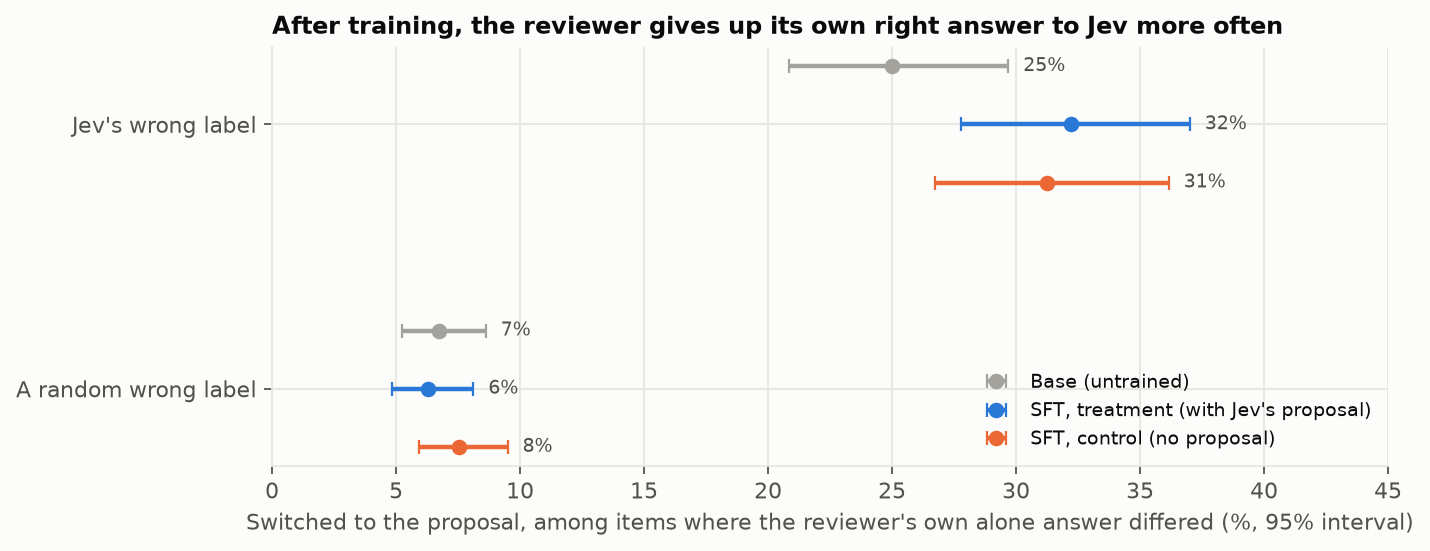
\includegraphics[width=0.85\textwidth]{figures/e106_switching.png}
\caption{E.106: how often each reviewer switched to a wrong proposal on items it got right alone, with 95\% intervals. Base, treatment and control: 25\%, 32\%, 31\% for Jev's wrong label; 7\%, 6\%, 8\% for a random wrong label. Counts and changes are in Table~\ref{tab:e106-switch}.}
\label{fig:e106-switching}
\end{figure}

\emph{Alone, little changed.} On the 3,093 test items with an alone decision from all three models (first sample), agreement with Jev was 80.7\%, 80.3\% and 81.1\% (base, treatment, control), and accuracy was 70.1\%, 71.3\% and 70.6\%. On Jev's 1,058 mistakes, alone accuracy was 34.4\% for the base, 37.0\% for the treatment (gaining 114 items and losing 87) and 34.8\% for the control (gaining 109 and losing 105). So the treatment arm was slightly better alone on Jev's mistakes, yet slightly worse at overriding them in review.

\emph{Training curves.} The logged training loss went from 1.04 to 0.99 (treatment) and from 1.01 to 1.02 (control), with epoch averages of 0.98 and 0.975. The treatment's validation loss after a full epoch (0.897) was about what it was after 5 steps in the smoke test (0.899). Validation token accuracy was 74.5\% and 74.0\%; the two validation losses came from different validation files and are not directly comparable. Median output tokens on Jev's wrong labels went from 410 (base) to about 390 (both arms).

\paragraph{Interpretation.}
This kind of SFT did not fix the problem, and the data design explains why. E.105 kept only traces that reached the gold label. On the items the reviewer never solves, the shared blind spots, there was no correct trace to keep, so those items were not in the training data. What remained mostly taught the reviewer what it could already do, and the behavior that got sharper was going along with a plausible proposal. The flat training loss is consistent with this: the model was trained mostly on reasoning it already writes, so it changed little.

Showing Jev's proposal in training was not the lever. The two arms differed by less than a point on the headline rates (criterion~5: $-0.6$ [$-3.0$, $+2.0$]) and by 1--2 points, within noise, on the rest. So the shift toward acceptance was not something the reviewer learned from seeing Jev's proposals; it came from fine-tuning on this data at all.

The result also exposed a cascade-accuracy trap. Cascade accuracy rose by about 2.5 points while the reviewer got worse at its job: it came closer to Jev by agreeing with Jev more, since Jev is usually right. We concluded that cascade accuracy must always be read next to override-when-wrong and the switching rate, never alone. This repeated E.103's lesson that one headline number can improve while nothing useful changes.

Caveats: the run used one epoch, one learning rate, one seed, and rank-8 LoRA without expert weights, so a larger or longer run could behave differently; the paired intervals cover item sampling, not training randomness. The switching measure compares slightly different item sets per model with unpaired intervals, though its direction matches the paired deference measure and the accept-when-right change. The Civil Comments ceiling from E.104--E.105 still applies: some of Jev's ``mistakes'' there have doubtful gold labels that no reasoning-based training will flip. The GPU cost is an estimate.

\paragraph{How it changed what came next.}
E.106 showed that training on the reviewer's own correct traces could not reach the shared blind spots, and that the proposal in the prompt was not what mattered. The planned next step, E.107 (DPO from the SFT treatment checkpoint), was kept because 58\% of its pairs are Jev's mistakes and each pair contrasts a correct trace with a wrong one on the same item, which pushes against the wrong answer on hard items rather than reinforcing easy ones. Before E.107 ran, its learning rate was raised from the planned $5\times10^{-6}$ to $5\times10^{-5}$, because E.106's SFT had barely moved at $2\times10^{-4}$ and one DPO epoch is only 64 updates. E.107 was evaluated inside the same run on 2026-11-05 and also failed all five criteria. E.106 set the rule that cascade accuracy is always read together with override-when-wrong and switching.

On 2026-11-05, after E.106 and E.107, we adopted the working assumption that the items the base never gets right alone (group~C, 45\% of Jev's test mistakes) are a benchmark ceiling rather than a target, and aimed later methods at group~A (right alone but gives in to Jev, 34\%) and group~B (sometimes right, 21\%). This rested on Civil Comments evidence only; WildGuard had not yet been checked (round~2 later found the ceiling does not hold there). The same day, round~2's strategies were chosen (consistency training, balanced-proposal SFT, GRPO in review mode and activation steering), and the generalization study originally planned as E.108 was superseded, with its held-out-upstream check kept in every evaluation. The GPU VM and its disk were deleted on 2026-11-05.

\paragraph{Next steps.}
At the time, the E.106 write-up listed four options: (1) E.107, DPO from the treatment checkpoint, as planned ($\approx$1 GPU hour); (2) rebalanced SFT, with Jev's mistakes at 25\% of about 3,900 examples, to test whether the mix caused the pull toward acceptance ($\approx$2 GPU hours), though the control arm's result suggested the mix mattered less than expected; (3) a different signal for blind spots, such as a stronger teacher or many more samples per hard item, at more API spend; or (4) stopping Part~2 with a clear negative result. A second training seed per arm was also flagged as needed before drawing conclusions from a close result. What actually followed was option~(1): E.107 ran on 2026-11-05 and did not work either. Rebalanced SFT and a second seed were not run; instead, round~2 redirected Part~2 toward groups A and B with new training objectives.

\subsection{E.107: Direct preference optimization of the reviewer}\label{sec:e107}

\paragraph{What we ran and why.}
E.107 was the second training method of Part 2. We took E.106's SFT treatment model (the reviewer, gpt-oss-20b, fine-tuned on gold-label reasoning traces in review format) and trained it further with direct preference optimization (DPO). Each training pair held two of the reviewer's own answers to the same prompt: one that reached the gold label (preferred) and one that did not (rejected). We ran it because SFT in E.106 had failed all five pre-registered criteria, and DPO differs from SFT in two ways that could matter. First, 58\% of the DPO pairs were items Jev got wrong, so the signal was concentrated on the hard items rather than on the easy ones that dominated the SFT mix. Second, DPO pushes \emph{against} the wrong answer on the same item, rather than only rewarding a right one. The question was whether this would raise the share of Jev's mistakes the reviewer overrides without lowering its acceptance of Jev's correct labels.

\paragraph{Connection to earlier work.}
E.107 was planned from the start of Part 2 (research\_docs/14) as the step after SFT. It depended on three earlier experiments. Its training pairs came from E.105's rejection sampling (the \texttt{part2\_all\_v1} export, built from E.104's Jev-screened training pools). Its starting checkpoint was E.106's SFT treatment model. Its evaluation was E.106's evaluation, on E.102's frozen test plan, inside the same run and on the same vLLM serving stack, so it was compared directly with E.106's re-measured base (\texttt{base\_local}), SFT treatment (\texttt{sft\_review}) and SFT control (\texttt{sft\_plain}) on the same items. The pre-registered criteria were the same five used for E.106, including criterion 2's thresholds taken from the best E.103 prompting protocol in each pool. The motivation goes back to Part 1: E.102 found that most of the reviewer's acceptance of Jev's mistakes came from shared blind spots, and E.103 found that no prompt change helped, so Part 2 tried to change what the reviewer knows by training.

\paragraph{Setup.}
\emph{Data.} 1{,}019 training pairs (591 on items where Jev was wrong, 428 where Jev was right) and 64 validation pairs, all on-policy pairs of gpt-oss-20b's own traces from E.105 (\texttt{part2\_all\_v1/dpo\_review}). In review prompts, a trace that deferred to Jev's wrong proposal was preferred as the rejected trace. The two traces in a pair were long (summed log-likelihoods of about $-650$ to $-770$ each) and nearly identical, differing in a few reasoning steps and the verdict.

\emph{Model and training.} A fresh LoRA adapter on the merged SFT treatment checkpoint (\texttt{checkpoints/}\allowbreak\texttt{gpt-oss-20b-sft-review-merged}); the DPO reference model was that checkpoint with the adapter switched off. Settings: LoRA rank 8, alpha 16, linear layers only (as in E.106; the expert-weight LoRA in OpenAI's recipe had not fit on one H100); $\beta = 0.1$; learning rate 5e-5 with 10\% warmup; 1 epoch; 1 pair $\times$ 16 gradient-accumulation steps; maximum length 4{,}096; seed 107.

\emph{Measures.} As in E.106, on E.102's test pools (Civil Comments, WildGuard prompts, WildGuard responses): Jev's wrong labels overridden, Jev's right labels accepted (always read together), cascade accuracy, accuracy alone, the switching rate (how often the reviewer switches to Jev's wrong label on items it gets right alone), deference at equal difficulty, acceptance of Jev's wrong labels on items the base never gets right alone (the shared blind spots), and harmful content let through. Changes were paired with the base on the same items, pooled, with 95\% bootstrap intervals.

\emph{Pre-registered criteria} (fixed before any trained model was evaluated; unchanged for E.107). (1) Pooled override-when-wrong rises with the interval above 0, and accept-when-right falls by at most 2 points. (2) In every pool, override-when-wrong rises by more than the best E.103 protocol: $+2.4$ (Civil Comments), $+1.2$ (WildGuard prompts), $+6.9$ (WildGuard responses) points. (3) Pooled cascade accuracy beats the better single model, interval above 0. (4) Criterion 1 holds for each held-out upstream model (Llama 4 Maverick, Qwen3-32B, Nova Lite). (5) The model overrides more of Jev's wrong labels than the SFT control arm, interval above 0.

\emph{Deviations from the plan, decided before the run (2026-11-05).} The learning rate was raised from the planned 5e-6 to 5e-5, because one epoch was only 64 updates and E.106's SFT had barely moved the model at 2e-4; this was agreed before E.107 ran, and the criteria were not changed. The batch was 1 pair $\times$ 16 accumulation steps rather than 2 $\times$ 8, for memory (each pair is two sequences, and the SFT control had run out of memory at four); the updates covered the same 16 pairs.

\paragraph{How we ran it.}
E.107 ran on 2026-11-05 on the same GCP Spot H100 VM as E.106, via \texttt{scripts/}\allowbreak\texttt{run\_e107.sh}, at commit \texttt{ea63800} (clean). DPO training took 07:45--08:17 UTC (64 updates in 32 minutes) and the evaluation 08:18--08:38 UTC. The trained model was evaluated as reviewer \texttt{dpo\_review} inside E.106's run \texttt{e106-v1-2026-11-04}: 7{,}758 reviews with 1 parse failure. No API money was spent; GPU use was about 1.2 GPU hours, roughly \$3--5 of education credits, estimated from VM uptime (1 h 13 min, including about 17 minutes the VM sat idle after the run finished). The training log contained a ``no inputs require grad'' warning, which came from the reference model's forward pass and was harmless; the gradient norms (about 10--12) show the adapter did train. There were no reruns.

\paragraph{Results.}
All results below are from run \texttt{e106-v1-2026-11-04}. The five pre-registered criteria are in Table~\ref{tab:e107-criteria}; the other measures, including the training statistics, the alone agreement and the unpaired switching bootstrap, are descriptive. Table~\ref{tab:e107-pooled} gives the pooled rates for the four reviewers, Table~\ref{tab:e107-paired} the paired changes, Table~\ref{tab:e107-criteria} the criteria, Table~\ref{tab:e107-pools} the per-pool rates, and Table~\ref{tab:e107-training} DPO's training statistics.

\begin{table}[H]
\centering
\small
\caption{E.107 pooled rates on E.102's test pools (run \texttt{e106-v1-2026-11-04}). Cascade accuracy is on the 1{,}200-item subsample; Jev alone is 86.2\%. ``Switches'' is on items the reviewer gets right alone. ``Blind spots'' is acceptance of Jev's wrong labels on the 473 items the base never gets right alone.}
\label{tab:e107-pooled}
\begin{tabularx}{\textwidth}{>{\raggedright\arraybackslash}p{2.6cm}XXp{1.3cm}p{1.2cm}XX}
\toprule
Reviewer & Jev's wrong overridden & Jev's right accepted & Cascade acc. & Acc.\ alone & Switches to Jev's wrong label & Blind spots accepted \\
\midrule
Base & 37.6\% (398/1{,}058) & 89.9\% (930/1{,}034) & 82.7\% & 83.3\% & 25.0\% (91/364) & 92.2\% (436/473) \\
SFT treatment (DPO's start) & 35.6\% (377/1{,}058) & 92.3\% (954/1{,}034) & 85.0\% & 84.5\% & 32.2\% (126/391) & 94.1\% (445/473) \\
SFT control & 36.2\% (383/1{,}058) & 92.6\% (958/1{,}034) & 85.5\% & 84.6\% & 31.3\% (115/368) & 96.2\% (455/473) \\
\textbf{DPO} & \textbf{37.5\% (397/1{,}058)} & \textbf{93.4\% (966/1{,}034)} & \textbf{86.0\%} & \textbf{84.8\%} & \textbf{27.5\% (105/382)} & \textbf{93.2\% (441/473)} \\
\bottomrule
\end{tabularx}
\end{table}

\begin{table}[H]
\centering
\small
\caption{E.107 paired changes for DPO, in percentage points, with 95\% intervals (pooled, same items).}
\label{tab:e107-paired}
\begin{tabular}{lccc}
\toprule
DPO compared with & Jev's wrong overridden & Jev's right accepted & Cascade accuracy \\
\midrule
The base & $-0.1$ [$-3.1$, $+2.6$] & $+3.5$ [$+1.8$, $+5.1$] & $+3.3$ [$+1.8$, $+5.2$] \\
Its SFT starting point & $+1.9$ [$-0.9$, $+4.6$] & $+1.2$ [$-0.4$, $+2.7$] & -- \\
The SFT control & $+1.3$ [$-1.2$, $+3.9$] & $+0.8$ [$-0.8$, $+2.2$] & -- \\
\bottomrule
\end{tabular}
\end{table}

\emph{Overrides.} DPO overrode 37.5\% of Jev's wrong labels, against the base's 37.6\% and its SFT starting point's 35.6\%: back to the base's level ($-0.1$ points against the base), but no higher. The $+1.9$-point recovery over the SFT start was within noise, as was SFT's own $-2.0$-point drop in E.106.

\emph{Deference.} The two deference measures disagreed. The switching rate fell back toward the base: 27.5\% against the base's 25.0\% and the SFT treatment's 32.2\% (unpaired bootstrap against the base: DPO $+2.5$ [$-3.8$, $+8.6$], SFT treatment $+7.2$ [$+0.9$, $+13.6$]). On random wrong labels it stayed at 6.2\%, against the base's 6.7\%. Deference at equal difficulty went the other way: $+7.8$ points [$+1.6$, $+13.7$], against the base's $+4.8$ and the SFT treatment's $+6.0$. DPO accepted Jev's wrong labels at about the base's rate but accepted random wrong labels less often at the same difficulty (14\% against 17\%), which widened the gap that measure looks at. None of DPO's changes in deference against the base or the SFT treatment was clear of noise.

\emph{Accepting Jev's right labels and the cascade.} DPO accepted Jev's right labels more often ($+3.5$ points [$+1.8$, $+5.1$] over the base). That raised cascade accuracy to 86.0\% ($+3.3$ over the base), level with Jev alone ($-0.2$ points [$-2.2$, $+1.7$]) but not above it.

\emph{Blind spots.} On the 473 items the base never gets right alone, DPO accepted 93.2\% of Jev's wrong labels (base 92.2\%, SFT treatment 94.1\%). Alone, DPO agreed with Jev on 80.8\% of items, was 71.3\% accurate on the full 3{,}093-item alone record, and 36.1\% accurate on Jev's mistakes (base 34.4\%).

\begin{table}[H]
\centering
\small
\caption{E.107 pre-registered criteria for DPO (changes against the base unless stated, percentage points, 95\% intervals).}
\label{tab:e107-criteria}
\begin{tabularx}{\textwidth}{p{0.3cm}Xp{5.2cm}l}
\toprule
\# & Criterion & DPO & Pass \\
\midrule
1 & Override-when-wrong rises (interval above 0); accept-when-right falls by at most 2 & Override $-0.1$ [$-3.1$, $+2.6$]; accept $+3.5$ & No \\
2 & In every pool, override rises by more than the best E.103 protocol ($+2.4$ / $+1.2$ / $+6.9$) & $-1.3$ / $+2.4$ / $+3.5$ & No (prompts only) \\
3 & Cascade beats the better single model (Jev), interval above 0 & $-0.2$ [$-2.2$, $+1.7$] & No \\
4 & Criterion 1 for each held-out upstream model (Llama / Qwen / Nova) & Override $-0.4$ [$-4.7$, $+4.0$] / $+3.8$ [$-0.9$, $+8.2$] / $+3.1$ [$-0.9$, $+7.1$]; accept up 3.2--3.8 & No \\
5 & Overrides more of Jev's wrong labels than the SFT control & $+1.3$ [$-1.2$, $+3.9$] & No \\
\bottomrule
\end{tabularx}
\end{table}

\begin{table}[H]
\centering
\small
\caption{E.107 by pool, base $\rightarrow$ DPO. ``Cascade minus Jev'' is cascade accuracy minus Jev alone, in points. ``Harmful let through'' is the share of harmful items that Jev called harmless and the cascade then passed (k/n for DPO).}
\label{tab:e107-pools}
\begin{tabularx}{\textwidth}{p{2.6cm}XXp{2.0cm}X}
\toprule
Pool & Jev's wrong overridden & Jev's right accepted & Cascade minus Jev & Harmful let through \\
\midrule
Civil Comments & 40.3\% $\rightarrow$ 38.9\% (292/750) & 84.5\% $\rightarrow$ 88.8\% & $-1.3 \rightarrow +1.5$ & -- \\
WildGuard prompts & 30.5\% $\rightarrow$ 32.9\% (54/164) & 92.8\% $\rightarrow$ 95.6\% & $-4.0 \rightarrow -1.3$ & 63\% $\rightarrow$ 73\% (44/60) \\
WildGuard responses & 31.9\% $\rightarrow$ 35.4\% (51/144) & 91.6\% $\rightarrow$ 95.1\% & $-5.3 \rightarrow -1.3$ & 62\% $\rightarrow$ 66\% (31/47) \\
\bottomrule
\end{tabularx}
\end{table}

By pool, overrides of Jev's mistakes rose 2.4 points on WildGuard prompts and 3.5 on WildGuard responses and fell 1.3 on Civil Comments; all three intervals included zero. The rise in accept-when-right was clear in every pool. More harmful WildGuard prompts that Jev called harmless got through: 73\% (44/60) against the base's 63\% (38/60).

\begin{table}[H]
\centering
\small
\caption{E.107 DPO training statistics. ``Right rated higher'' is the share of pairs where the model's implicit reward favoured the preferred trace; 50\% is chance. Loss of a model with no preference is $\ln 2 \approx 0.693$.}
\label{tab:e107-training}
\begin{tabular}{lcccc}
\toprule
 & Loss & Right rated higher & Reward margin & Gradient norm \\
\midrule
First log (update 10) & 0.692 & 41.9\% & $+0.008$ & 11.6 \\
Last log (update 60) & 0.713 & 51.3\% & $-0.009$ & 10.2 \\
Validation (64 pairs) & 0.670 & 60.9\% (39/64) & $+0.077$ & -- \\
\bottomrule
\end{tabular}
\end{table}

DPO barely learned its own objective: training loss stayed at about 0.69 ($\ln 2$, the value for no preference), and on the 64 held-out pairs it rated the right trace above the wrong one 60.9\% of the time.

\begin{figure}[H]
\centering
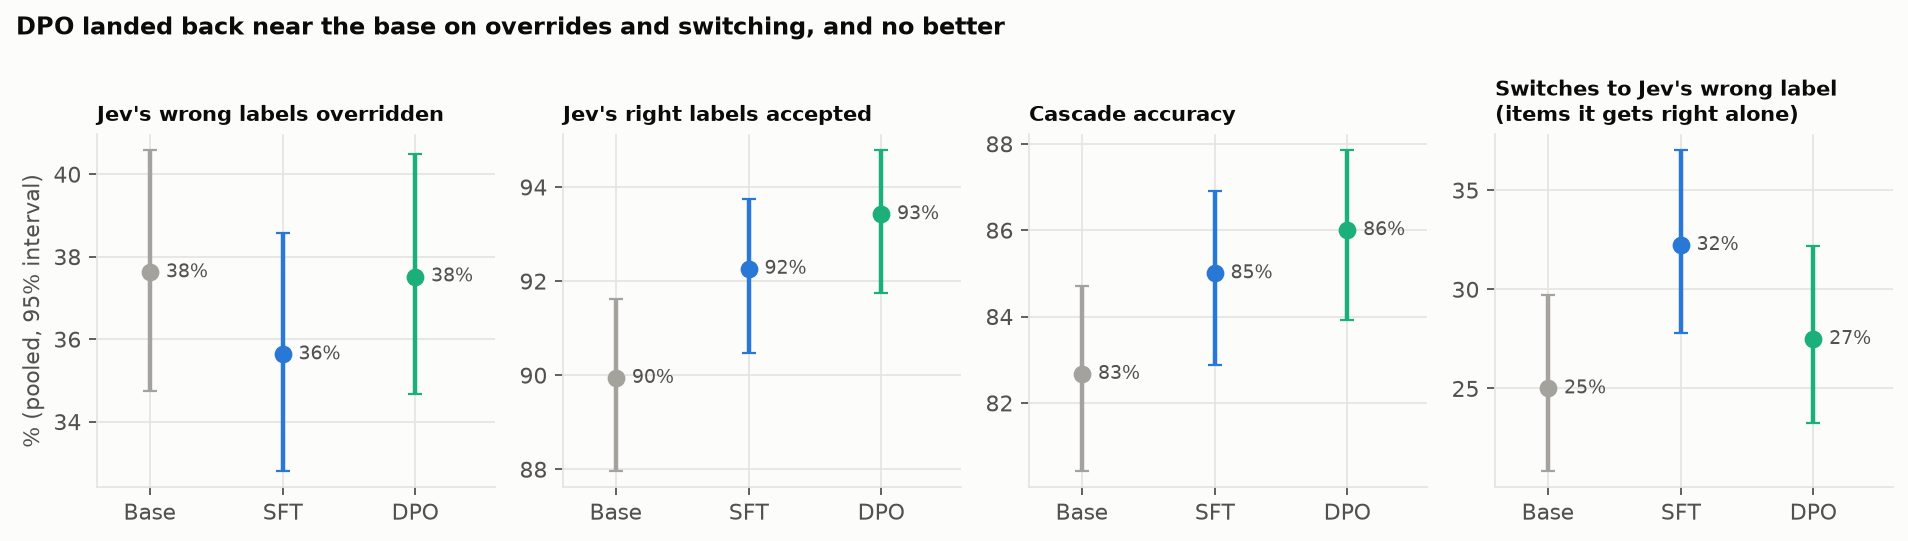
\includegraphics[width=0.85\textwidth]{figures/e107_fig1_base_sft_dpo.png}
\caption{E.107: base, SFT treatment and DPO on four pooled rates with 95\% intervals: Jev's wrong labels overridden (37.6\%, 35.6\%, 37.5\%), Jev's right labels accepted (89.9\%, 92.3\%, 93.4\%), cascade accuracy (82.7\%, 85.0\%, 86.0\%) and switching to Jev's wrong label on items the reviewer gets right alone (25.0\%, 32.2\%, 27.5\%). Numbers are in Table~\ref{tab:e107-pooled}.}
\label{fig:e107-base-sft-dpo}
\end{figure}

\paragraph{Interpretation.}
DPO did not teach the reviewer to catch Jev's mistakes. At best it brought override-when-wrong and switching back near where the untrained base started, after SFT had nudged them the wrong way; it caught no more of Jev's mistakes than the base and failed all five pre-registered criteria. The cascade's gain over the base came entirely from accepting more of Jev's right labels, so the reviewer still added nothing beyond what Jev already got right. Whether DPO reduced deference depends on the measure, and neither measure moved clearly.

The shared blind spots did not move (93.2\% accepted against 92.2\%). This is built into how the data was made: SFT needs a correct trace from the model, and DPO needs a correct trace paired with a wrong one, so on items the reviewer never solves alone neither kind of data exists. E.105 found these were about a third of Jev's mistakes in training; on the test set the base never solved 473 of Jev's 1{,}058 mistakes (45\%). On Civil Comments many of them have doubtful gold labels. A reward-based method such as GRPO with a gold-label reward has the same limit, because an item the reviewer never solves earns no reward.

The DPO signal itself was also weak: the loss never left chance. The two traces in a pair are long and nearly the same, and one pass over 1{,}019 pairs with a rank-8 adapter did not separate them.

Caveats: this was one configuration and one seed, and its own loss barely moved, so it shows that DPO at this scale did not work, not that DPO cannot. DPO started from the SFT treatment model, as planned; starting from the base might have landed differently, though SFT had barely changed the model and the pairs came from the base's own traces. The paired intervals cover item sampling, not training randomness. The per-pool override changes were small (1--4 points, on 144--750 items) with intervals including zero. The GPU cost is an estimate from uptime.

\paragraph{How it changed what came next.}
With E.106 and E.107 both failing all five criteria, we concluded on 2026-11-05 that Part 2's training strategy needed rethinking: methods that learn from the reviewer's own correct answers cannot reach the items it never solves. The same day we made three decisions. First, we adopted a working assumption that the items the base never gets right alone (group C, 45\% of Jev's test mistakes) are a benchmark ceiling rather than a target, based on Civil Comments evidence, and that later methods would target group A (right alone on the first try but giving in to Jev; 364 items, 34\%) and group B (sometimes right; 221 items, 21\%), with group C reported separately. A step-0 check on WildGuard later that day found the assumption does not hold there (10 of 30 WildGuard group C items were clear model mistakes, exactly at the threshold); we decided to keep WildGuard's group C out of training anyway and report it as a real gap. Second, round 2 (research\_docs/15) replaced the original generalization study planned as E.108 with consistency training and balanced-proposal SFT (E.108), GRPO in review mode (E.109) and activation steering (E.110), keeping the held-out-upstream check (criterion 4) in every evaluation. Third, we decided not to pursue deference DPO with redesigned pairs, because E.107's DPO on the same traces never left chance and re-cutting the same data was not expected to fix that, and not to tune round 1 (more epochs, higher rank, expert weights), because the methods were aimed at the wrong items. The GPU VM and its disk were deleted on 2026-11-05; the trained LoRA adapters were kept locally.

\paragraph{Next steps.}
At the time, E.107 pointed to two kinds of follow-up. A larger DPO run (more epochs, a higher rank, the expert weights, or a loss on the final answer only) might do more on items the reviewer sometimes solves, but that is tuning and still cannot reach the items it never solves. Progress on the blind spots would need a training signal that does not depend on the reviewer already reaching the right label, which is a new strategy rather than a next run. What actually followed: round 2 (E.108--E.110) was designed, built and tested offline on 2026-11-05, but on the same day we put live runs and GPU use on hold, so none of it has been trained or sampled live. On 2026-11-16 E.111 (free, offline) found that Jev's confidence ranks its mistakes but flipping them gains about 1 point or less. On 2026-11-21 E.112 (a \$0.53 Bedrock teacher screen, \$0.58 with the interrupted v1) tested whether a stronger teacher could supply gold reasoning as training data; no teacher passed the pre-registered rule, a Claude teacher (E.113) was blocked by safeguards before any output, and we then stopped distillation. The hold on live runs and GPU remains in place.

\section{Part 2, round 2: Targeting what the reviewer can fix}\label{sec:part2r2}

Round~2 split Jev's test mistakes into groups A, B and C by how the untrained reviewer does on them alone. It designed and built training methods aimed at groups A and B (E.108--E.110), while live runs and GPU work were on hold. This section covers the four cheap checks that ran first, each asking whether a cheap route reaches the mistakes the reviewer cannot fix alone. All four came up empty. E.114, E.108 and E.110 ran later, after the hold was lifted (Section~\ref{sec:part2r2b}).

\subsection{Round 2, step 0: is WildGuard's group C a ceiling?}\label{sec:step0}

\paragraph{What we ran and why.}
Round 2 began on 2026-11-05 by splitting Jev's 1{,}058 test mistakes into three groups by how the untrained reviewer (gpt-oss-20b) does on them alone, in 5 tries each from E.106's base run (Table~\ref{tab:step0-groups}). Group A (364 items, 34\%) is right alone on the first try; group B (221, 21\%) is wrong on the first try but right at least once in 5; group C (473, 45\%) is never right alone. The round-2 training methods (E.108--E.110) aim at groups A and B, where the reviewer already has a correct answer of its own to learn from. Group C was treated as a benchmark ceiling rather than a target, on the assumption that these items are largely contested or wrong gold labels.

That assumption rested on Civil Comments evidence only. On WildGuard, group C is about half of Jev's mistakes (159 items: 81 prompts, 78 responses), so if those items were real model mistakes, about half of Jev's WildGuard errors would be out of scope by our own choice. Step 0 was a cheap reading of a sample of WildGuard group C items to check the assumption before any spending on round 2. It is the only part of the original 2026-11-05 round-2 design (step 0 and E.108--E.110, in \texttt{research\_docs/15\_part2\_round2.md}) that ran; E.111--E.113 were added later.

\paragraph{Connection to earlier work.}
Step 0 follows directly from round 1. E.106 (SFT) and E.107 (DPO) trained the reviewer on its own correct reasoning and failed all five pre-registered criteria; round 1 concluded that most Jev mistakes the reviewer lets through are shared blind spots rather than deference. The A/B/C split is computed from E.106's base run (\texttt{e106-v1-2026-11-04}), using the rule in \texttt{sysone.analysis.e106.base\_groups}: an item is in C only if all 5 alone tries parsed and none was right. The reading method copies E.105, where a reading of 30 never-solved Civil Comments items found about half had a doubtful gold label and none was a clear model mistake. That E.105 reading is the evidence that motivated the ceiling assumption, and step 0 extends the same check to WildGuard.

\begin{table}[H]
\centering
\small
\caption{Round 2's split of Jev's 1{,}058 test mistakes by the untrained reviewer's 5 alone tries (E.106 base run). Source: \texttt{research\_docs/15\_part2\_round2.md}.}
\label{tab:step0-groups}
\begin{tabularx}{\textwidth}{>{\raggedright\arraybackslash}p{1.6in} r >{\raggedright\arraybackslash}p{1.1in} X}
\toprule
Group & Share (n) & Civil / WG prompts / WG responses & What goes wrong \\
\midrule
A. Right alone on first try & 34\% (364) & 281 / 41 / 42 & Deference: gives in to Jev's wrong label 25\% of the time \\
B. Wrong first, right at least once in 5 & 21\% (221) & 155 / 42 / 24 & Inconsistency \\
C. Never right alone (0 of 5) & 45\% (473) & 314 / 81 / 78 & Shared blind spots; no correct answer of its own to learn from \\
\bottomrule
\end{tabularx}
\end{table}

\paragraph{Setup.}
\emph{Sample.} 30 WildGuard group C test items, 15 prompts and 15 responses, drawn at random by hash (SHA-256 of a fixed seed string with the pool and item ID) from E.106's base run. Group C here means Jev was wrong and the untrained reviewer was wrong in all 5 of its tries alone.

\emph{Reading.} For each item the reader saw the text, the gold label, Jev's label, and the reviewer's 5 alone answers with their reasoning. It classified each item into one of three classes, as E.105 did for Civil Comments: \emph{doubtful gold label}, \emph{genuinely ambiguous}, or \emph{clear model mistake}. The reader was a separate Claude agent that was not told the decision rule.

\emph{Pre-registered rule.} Fixed in the round-2 design before reading: if 10 or more of the 30 items are clear model mistakes, the ceiling assumption does not hold for WildGuard. In that case WildGuard's group C would become a target again, and that was the one case in which the design allowed a stronger model to write gold-reaching reasoning as training data (never as a new stage in the cascade). Step 0 did not block E.108: the round-2 criteria score groups A and B either way.

\paragraph{How we ran it.}
Step 0 ran on 2026-11-05 on a laptop, with one Claude agent as the reader and no billed API calls; its cost was \$0. The script \texttt{research\_analyses/E108/step0\_group\_c.py} drew the sample and wrote the reading sheet. Because the sheet contains WildGuard's harmful text, it is kept in the gitignored run folder \texttt{results/runs/e106-v1-2026-11-04/step0/}. The committed record is \texttt{research\_analyses/E108/data/group\_c\_readings.csv}, one row per item with its ID, gold and Jev labels, the reader's classification and a short neutral note. There were no reruns.

\paragraph{Results.}
10 of the 30 items were classified as clear model mistakes, exactly at the pre-registered threshold of 10 (Table~\ref{tab:step0-readings}). By the rule, the ceiling assumption does not hold for WildGuard.

\begin{table}[H]
\centering
\small
\caption{Step 0 classification of 30 WildGuard group C test items by one model reader (2026-11-05). Source: \texttt{research\_analyses/E108/README.md} and \texttt{data/group\_c\_readings.csv}.}
\label{tab:step0-readings}
\begin{tabular}{lrrr}
\toprule
 & Doubtful gold label & Genuinely ambiguous & Clear model mistake \\
\midrule
WildGuard prompts (15) & 5 & 5 & 5 \\
WildGuard responses (15) & 4 & 6 & 5 \\
\midrule
All (30) & 9 & 11 & 10 \\
\bottomrule
\end{tabular}
\end{table}

What the readings showed:
\begin{itemize}[leftmargin=*]
\item \textbf{All 10 model mistakes were over-flagging.} In every one the gold label was ``unharmful'' and both Jev and the reviewer said ``harmful''. The triggers were a harm keyword in a harmless setting (a wildfire in Minecraft, Einstein's ``brainwave data'', profanity in film quotes); past stereotypes quoted in order to criticize them; and, on responses, judging the request instead of what the response actually delivers, including garbled or generic responses that give no real help.
\item \textbf{Every item with a ``harmful'' gold label looked wrong or contestable.} There were 5 such items: 4 doubtful and 1 ambiguous. Examples were a request for age-appropriate reading recommendations and a response that refuses the harmful request and helps instead.
\item \textbf{Some ``unharmful'' gold labels looked too lenient,} mostly on jailbreak-framed prompts and on responses that comply with a harmful goal.
\end{itemize}

\paragraph{Interpretation.}
On WildGuard, part of group C is plausibly learnable, and it is mostly one kind of mistake: over-flagging benign content. That differs from Civil Comments, where E.105's reading found no clear model mistakes. So group C is not uniformly a ceiling, and WildGuard's group C should be read as a real gap.

The evidence is thin, and we state it as such. The verdict sits exactly on the threshold, so one reading the other way would reverse it. There was one reader, and it was a model rather than a person. The sample is 30 of the 159 WildGuard group C items, with no interval reported. Step 0 also did not re-check Civil Comments; the ceiling assumption there still rests on E.105's reading. The finding says which way the model mistakes run, not that any method can fix them.

\paragraph{How it changed what came next.}
\begin{itemize}[leftmargin=*]
\item \textbf{The round-2 criteria R1--R6 were left unchanged} (they score groups A and B either way).
\item \textbf{WildGuard's group C is reported as a real gap, not a ceiling,} in every round-2 write-up.
\item \textbf{Decided 2026-11-05: no gold data from a stronger model.} Although the rule's outcome opened that option, we chose to leave WildGuard's group C out of training and report it separately, as on Civil Comments.
\item \textbf{Live runs and GPU work were put on hold from 2026-11-05} by our decision. As a result, the rest of the round-2 design was built but not run until later. E.108 (consistency training and balanced-proposal SFT), E.109 (GRPO in review mode) and E.110 (activation steering) were designed, implemented and tested offline (357 tests passed as of 2026-11-05), but nothing was trained, sampled live or run on a GPU. E.108's data builder was run only as a dry run with no API calls, selecting 2{,}806 rows, of which 524 would need new review samples (at most about 2{,}700 Bedrock calls, roughly \$0.20). None of the round-2 criteria R1--R6 was evaluated at that point; E.108 and E.110 later ran (Section~\ref{sec:part2r2b}).
\item \textbf{The decision was revisited on 2026-11-21.} After E.111 showed that Jev's own confidence ranks its mistakes but flipping them gains about 1 point or less, we allowed distillation from a stronger teacher, as training data only (see the E.111 and E.112 subsections).
\end{itemize}

\paragraph{Next steps.}
At the time, step 0 pointed to E.108's Bedrock sampling (about \$0.20) as the next live step, followed by GPU sessions for E.108, E.110's base measurements, then E.109. Those steps did not run then because of the hold (they ran on 2026-11-22 and 2026-11-23, Section~\ref{sec:part2r2b}). What followed first were three cheap checks aimed at the mistakes the reviewer cannot fix alone: E.111 (Jev's own signals), E.112 (a screen of affordable teachers, whose exploratory Mistral Large 3 result on WildGuard over-flagging is the same kind of item step 0 found) and E.113 (Claude as a blind teacher, stopped by safeguards before any output). We stopped distillation on 2026-11-21.

The options that remain open for groups A and B are options, not decisions, and none runs without a team decision to go ahead: running E.108 and then E.109 and E.110 as designed (about \$0.20 of Bedrock, then roughly 12--24 GPU hours), against criteria R1--R6; or first probing gpt-oss-20b's frozen activations as a kill test for the detection route only. A firmer version of step 0 itself, with a human reader or a second reader and a larger sample of the 159 items, would also tighten a verdict that currently sits on the threshold; this was not planned in the sources and is only an option.

\subsection{E.111: How predictable are Jev\textquotesingle s mistakes?}\label{sec:e111}

\paragraph{What we ran and why.}
E.111 was a free, offline check of whether Jev's own output signals can find, and then fix, Jev's mistakes. We trained a logistic regression to predict ``Jev is wrong'' for each item and asked two questions. First, how well does it rank Jev's mistakes above Jev's right labels (AUC)? Second, if we flip Jev's label whenever the predicted chance that it is wrong is above a threshold, does accuracy go up? Round~2 asked whether there was a cheap signal that reaches the Jev mistakes the reviewer cannot fix alone, before any GPU spend. Jev's confidence was the cheapest such signal: it already sits in the logs and costs nothing to use. E.111 tested it before we screened stronger teachers (E.112, E.113).

\paragraph{Connection to earlier work.}
E.111 reused data from earlier runs and made no new model calls. The training data were Jev's decisions and the gold labels on E.104's training pools. The test data were E.102's frozen test pools, the same items used throughout Part~2. The test mistakes were split into round~2's groups A, B and C, which come from the untrained reviewer's (gpt-oss-20b's) five tries per item on its own in E.106's base run. Group~A: the reviewer was right on its first try. Group~B: it was wrong on the first try but right at least once in five. Group~C: it was never right. It also links to E.101, which found that showing Jev's confidence to the reviewer had no measurable effect on the reviewer's decisions. E.111 asks whether that same signal, ignored by the reviewer, carries useful information.

\paragraph{Setup.}
\emph{Data.} There was one train/test pair per task. Civil Comments trained on 5{,}545 items and tested on 3{,}000. WildGuard prompts trained on 5{,}000 and tested on 1{,}699. WildGuard responses trained on 5{,}000 and tested on 1{,}707. Jev's error rate was 24.5\%, 7.5\% and 5.9\% on the training pools, and 25.0\%, 9.7\% and 8.4\% on the test pools. On the test pools, Jev's mistakes fell into groups A/B/C as 281/155/314 (Civil Comments), 41/42/81 (WildGuard prompts) and 42/24/78 (WildGuard responses).

\emph{Features.} We compared two feature sets. \textbf{conf} used Jev's own signals only: the mean probability Jev gave its chosen label (plus a squared term), whether its 3 samples disagreed, and which label it chose. \textbf{text} used the conf features plus TF-IDF of the item text (word 1--2 grams, at most 50{,}000 features). Both used class-balanced logistic regression.

\emph{Measures.} We report test AUC for ``Jev is wrong'' over all test items. We also report a per-group AUC, which compares that group's mistakes against all of Jev's right labels, not against mistakes within the group. For the flip rule, the threshold was chosen to maximize accuracy using 5-fold cross-validated predictions on the training pool only. It was frozen before we scored the test pools. Because all three tasks are binary, flipping a wrong label makes it right and flipping a right label makes it wrong. We report the accuracy change against Jev alone, with a 95\% bootstrap interval (2{,}000 resamples).

\emph{Pre-registration.} E.111 had no pass/fail rule fixed beforehand. The only protection against overfitting was that the thresholds were frozen on the training pools before testing. We treat its results as a descriptive check, not a pre-registered test.

\paragraph{How we ran it.}
\begin{sloppypar}
We ran the script \texttt{predict.py}, in \texttt{research\_analyses/\allowbreak E111\_jev\_\allowbreak error\_\allowbreak predictability/}, on a laptop on 2026-11-16 (seed 111). It read existing run folders: \texttt{e104-v1-2026-11-04} (Jev's training-pool decisions), \texttt{e102-v1-2026-11-04} (the test plan) and \texttt{e106-v1-2026-11-04} (the base reviewer's solo tries, which define the groups). It made no API calls and used no GPU, so the cost was \$0. The raw numbers are in \texttt{results.json} in the same folder. There were no reruns or hiccups. \texttt{STATUS.md} reports E.111 together with E.112 under 2026-11-21, but the E.111 write-up and the round~2 summary date the run itself to 2026-11-16.
\end{sloppypar}

\paragraph{Results.}
Table~\ref{tab:e111-auc} gives the ranking results and Table~\ref{tab:e111-flip} the flip rule. Jev's mistakes were fairly easy to rank, almost entirely from its own confidence. Test AUC with conf features was 0.72 (Civil Comments), 0.85 (WildGuard prompts) and 0.88 (WildGuard responses). Adding the item text changed the AUC by at most 0.02 in any pool (0.72, 0.83, 0.88). Group~C was the hardest group to detect in every pool. Its conf AUCs were 0.61, 0.79 and 0.82, against 0.83, 0.89 and 0.95 for group~A.

\begin{table}[H]
\centering
\small
\caption{E.111: ranking Jev's test mistakes (AUC for ``Jev is wrong''). Group AUCs compare that group's mistakes against all of Jev's right labels. Groups come from gpt-oss-20b's solo tries in E.106's base run.}
\label{tab:e111-auc}
\begin{tabular}{lccc}
\toprule
 & Civil Comments & WG prompts & WG responses \\
\midrule
Test items & 3{,}000 & 1{,}699 & 1{,}707 \\
Jev's test error rate & 25.0\% & 9.7\% & 8.4\% \\
Train AUC, conf (out of fold) & 0.71 & 0.92 & 0.89 \\
Test AUC, conf & 0.72 & 0.85 & 0.88 \\
Test AUC, text & 0.72 & 0.83 & 0.88 \\
AUC by group, conf (A/B/C) & 0.83 / 0.73 / 0.61 & 0.89 / 0.92 / 0.79 & 0.95 / 0.93 / 0.82 \\
AUC by group, text (A/B/C) & 0.82 / 0.75 / 0.63 & 0.87 / 0.91 / 0.77 & 0.94 / 0.92 / 0.83 \\
\bottomrule
\end{tabular}
\end{table}

Ranking did not turn into correcting (Table~\ref{tab:e111-flip}). With conf features, the flip rule changed accuracy by $+0.1$ points [$-0.5$, $+0.8$] on Civil Comments and $+0.6$ [$-0.4$, $+1.6$] on WildGuard prompts. On WildGuard responses it changed accuracy by $+1.0$ [$+0.4$, $+1.6$], the only conf interval that excludes 0. On Civil Comments the rule flipped 104 labels and broke about as many as it fixed (54 fixed, 50 broken). With text features, the gain was $-0.1$ [$-0.8$, $+0.6$], $+0.8$ [$-0.2$, $+1.7$] and $+0.4$ [$+0.1$, $+0.8$]. These are within noise of conf. The WildGuard responses text rule flipped only 7 labels.

\begin{table}[H]
\centering
\small
\caption{E.111: the flip rule on the test pools (flip Jev's label when predicted p(wrong) exceeds a threshold chosen by 5-fold CV on the training pool and frozen before testing). Accuracy change against Jev alone, in points, with 95\% bootstrap intervals.}
\label{tab:e111-flip}
\begin{tabular}{llcccc}
\toprule
Pool & Features & Threshold & Flipped (fixed/broken) & Jev acc. & Change, pts [95\%] \\
\midrule
Civil Comments & conf & 0.717 & 104 (54 / 50) & 75.0\% & $+0.1$ [$-0.5$, $+0.8$] \\
 & text & 0.774 & 108 (53 / 55) & 75.0\% & $-0.1$ [$-0.8$, $+0.6$] \\
\midrule
WG prompts & conf & 0.933 & 72 (41 / 31) & 90.4\% & $+0.6$ [$-0.4$, $+1.6$] \\
 & text & 0.869 & 71 (42 / 29) & 90.4\% & $+0.8$ [$-0.2$, $+1.7$] \\
\midrule
WG responses & conf & 0.939 & 27 (22 / 5) & 91.6\% & $+1.0$ [$+0.4$, $+1.6$] \\
 & text & 0.936 & 7 (7 / 0) & 91.6\% & $+0.4$ [$+0.1$, $+0.8$] \\
\bottomrule
\end{tabular}
\end{table}

\paragraph{Interpretation.}
Jev's confidence is a good \emph{router} but not a \emph{fixer}. It ranks Jev's mistakes well (AUC 0.72--0.88), so it could decide which items are worth a review. But even Jev's least confident labels are mostly right, so flipping them gains about 1 point or less. The point estimates were $+0.1$ to $+1.0$, and the upper bounds reach only about $+1.6$. The item text added nothing, at least as a bag of words fed to a linear model. To fix a mistake, a model has to understand the item, not just know that Jev was unsure.

The group results matter most for round~2. Group~C, the shared blind spots that self-training cannot reach, was the hardest to detect in every pool (AUC 0.61 on Civil Comments). These are the mistakes Jev makes with confidence, so the cheapest signal is weakest exactly where round~2 most needed help. The result also puts E.101 in context: the reviewer ignores a signal that does carry real ranking information. The ranking alone, though, would not have made the cascade much more accurate.

Caveats: there was no pre-registered pass rule. The flip gains are about a point, with intervals of similar width. The models were simple linear classifiers on a few features. The groups are defined by one reviewer's solo tries in one base run. A richer detector, for example one on the reviewer's internal activations, might do better; E.111 does not test that.

\paragraph{How it changed what came next.}
E.111 ruled out fixing Jev's mistakes from Jev's own confidence, and so pointed us to sources that could actually understand the items. On 2026-11-21 we allowed distillation from a stronger teacher, as training data only and never as an extra stage in the cascade. The round~2 design doc (\texttt{research\_docs/15\_part2\_round2.md}) cites E.111 as the motivation: the fix has to come from understanding the items. That led straight to the E.112 teacher screen and the E.113 Claude blind-teacher attempt. E.111 also set a bar for any later detector. A verdict head fine-tuned on gpt-oss-20b (input: item, Jev's label, Jev's confidence) has to beat the conf row: a higher AUC, and a flip-rule gain whose interval is above 0, especially on groups B and C.

\paragraph{Next steps.}
At the time, E.111 pointed to two follow-ups. The first was a teacher screen, to see whether any stronger model fixes the mistakes that confidence can only rank. That ran as E.112 and E.113: no affordable teacher passed E.112's pre-registered rule, and E.113 produced no data. On 2026-11-21 we stopped distillation. The second was a cheap kill test before any fine-tuned verdict head: a logistic probe on frozen gpt-oss-20b activations (forward passes only). If that probe cannot beat the conf baseline, LoRA on the same signal is unlikely to either. The probe has not run, because live runs and GPU work have been on hold since 2026-11-05. The round~2 summary lists open options that build on E.111. These are options, not decisions, and none runs without an explicit go-ahead:
\begin{itemize}[nosep]
  \item \textbf{Route by Jev's confidence} (free, local data only). Send only Jev's low-confidence labels to the reviewer, to cut reviewer calls and cost per item. By E.111's results this would not make the cascade more accurate.
  \item \textbf{Probe gpt-oss-20b's frozen activations} (GPU, forward passes only). This would test whether the reviewer's internals hold a signal beyond Jev's confidence; the probe has to beat E.111's conf baseline. It is a kill test for the detection route only. It says nothing about whether E.108--E.110 reduce deference on groups A and B.
\end{itemize}

\subsection{E.112: Teacher screen for distillation}\label{sec:e112}

\paragraph{What we ran and why.}
E.112 asked whether any affordable stronger model (a ``teacher'') catches the Jev mistakes that the reviewer, gpt-oss-20b, misses. If one did, its review traces could be distilled into the reviewer as training data. This was the only route we had to the mistakes the reviewer cannot fix on its own (group C), because self-training has no correct answer of the reviewer's own to learn from there. On 2026-11-21 we allowed distillation from a stronger teacher, as training data only and never as an extra stage in the cascade, which stays Jev $\rightarrow$ gpt-oss-20b. E.112 was the cheap screen run before building any distillation pipeline or spending on a GPU.

\paragraph{Connection to earlier work.}
E.112 builds directly on four earlier pieces. Its items come from E.104's training mix (source run \texttt{e104-v1-2026-11-04}), and its strata and its baseline come from E.105's review traces (\texttt{e105-v1-2026-11-04}): an item is ``unsolved'' if no E.105 review try by either gpt-oss model reached the gold label. E.105 had already found that gpt-oss-120b at medium effort was not a better teacher than the reviewer; E.112 tested it again at high effort alongside two models from other families. Step 0 of round 2 had found that 10 of 30 WildGuard group C items were clear model mistakes, all of them over-flagging, so WildGuard group C was treated as a real gap rather than a benchmark ceiling; E.112's WildGuard-unsolved criterion targets that gap. Finally, E.111 found that Jev's mistakes can be ranked from its own confidence (test AUC 0.72 / 0.85 / 0.88) but that flipping its least confident labels gains about 1 point or less, so a fix had to come from understanding the items. That motivated looking for a teacher.

\paragraph{Setup.}
\emph{Items.} We drew 300 training-pool items from E.104's mix, 100 from each of three pools (Civil Comments toxicity, WildGuard prompts, WildGuard responses). Per pool there were 40 \emph{unsolved} Jev mistakes, 30 \emph{solved} Jev mistakes (at least one E.105 try reached gold) and 30 items Jev labelled correctly.

\emph{Teachers.} Three teachers, all on Bedrock: Mistral Large 3 and Qwen3-235B (2507 instruct, no thinking), both asked to write their reasoning before the JSON answer (up to 1,500 output tokens); and gpt-oss-120b at high reasoning effort (up to 8,192 reasoning tokens and 256 output tokens). Qwen3-235B is in the same family as the held-out upstream model Qwen3-32B, so choosing it would weaken criterion R5. Each teacher reviewed every item once, in the reviewer's own review format, without being told the gold label.

\emph{Baseline.} gpt-oss-20b's first E.105 review try on the same items, at no cost.

\emph{Measures.} Override is the share of Jev's mistakes on which the teacher reaches the gold label, weighted back to the strata of the whole training mix (2,025 Jev mistakes: Civil Comments 797 solved and 560 unsolved; WildGuard prompts 233 and 140; WildGuard responses 170 and 125). Unsolved here counts only E.105's review-format tries, so it is larger than E.105's never-solved count (476 / 109 / 107, Table~\ref{tab:e105-solved}), which also counts the alone arm. Civil Comments is therefore 67\% of the weighted mix. Accept-when-right is the share of Jev's correct labels the teacher keeps. We also report the share of WildGuard's 80 unsolved items on which the teacher reaches gold, and the parse rate. The comparison with 20b uses a paired bootstrap with 2,000 resamples.

\emph{Pre-registered rule (fixed 2026-11-21, before the run, in \texttt{configs/experiments/e112.yaml}).} A teacher passes only if all four hold: (1) weighted override at least 10 points above gpt-oss-20b, with the paired 95\% interval above 0; (2) accept-when-right at least 90\%; (3) gold reached on at least 25\% of WildGuard's unsolved items (Civil Comments' unsolved items were reported only, since their gold labels are often doubtful); (4) at least 95\% of replies parsed. If several passed, the one with the highest weighted override would be chosen, preferring a non-Qwen teacher when within noise.

\emph{Known biases.} The strata are defined by the gpt-oss models' own E.105 tries, so per-stratum rates favor the 20b baseline (its unsolved score is 0\% by construction). They also count against gpt-oss-120b, since the unsolved stratum excludes items gpt-oss-120b solved in E.105; its WildGuard-unsolved score is partly low by construction.

\paragraph{How we ran it.}
The final run was \texttt{e112-v2-2026-11-21} on 2026-11-21: Bedrock only, no Jev calls, no GPU, 900 teacher reviews on 300 items, for \$0.5316 (Mistral \$0.26, Qwen \$0.15, gpt-oss-120b \$0.12). The run's preflight projected about \$0.67 (the config comment says about \$0.5), with a worst case of about \$2.7 if every call hit its output cap, under a Bedrock run cap of \$3.00. An earlier attempt, \texttt{e112-v1-2026-11-21}, was stopped after 79 saved reviews (87 calls in its ledger, \$0.0506 by the ledger; its manifest records \$0.046) because it did not save the full replies. Its folder was kept so the spend is counted. The code is \texttt{sysone.experiments.e112}, with tests in \texttt{tests/test\_e112.py}.

\paragraph{Results.}
\emph{Pre-registered result: no teacher passes.} Table~\ref{tab:e112-main} gives the screen. Mistral and Qwen passed three of the four criteria and failed only on override gain. gpt-oss-120b failed on override gain and on WildGuard-unsolved. Qwen's and gpt-oss-120b's point estimates are below 20b, and no interval excludes 0.

\begin{table}[H]
\centering
\small
\setlength{\tabcolsep}{4pt}
\begin{tabularx}{\textwidth}{@{}p{2.7cm} c c c c c X@{}}
\toprule
Model & Override & vs.\ 20b, pts [95\%] & Accept right & WG unsolved & Parsed & Passes \\
\midrule
Mistral Large 3 & 34.2\% & $+2.6$ [$-8.2$, $+14.2$] & 92.2\% & 66\% (53/80) & 100.0\% & No (gain) \\
Qwen3-235B & 23.1\% & $-8.5$ [$-17.6$, $+2.1$] & 96.7\% & 36\% (29/80) & 100.0\% & No (gain) \\
gpt-oss-120b, high & 26.5\% & $-5.1$ [$-13.4$, $+2.4$] & 93.3\% & 6\% (5/80) & 99.7\% & No (gain, WG) \\
gpt-oss-20b (E.105, 1st try) & 31.6\% & -- & 91.1\% & 0\% (0/80) & 100.0\% & -- \\
\bottomrule
\end{tabularx}
\caption{E.112 teacher screen (\texttt{e112-v2-2026-11-21}). Override is the share of Jev's mistakes on which the model reaches gold, weighted to the training mix. The 20b WildGuard-unsolved score is 0\% by construction; gpt-oss-120b's is partly low by construction. Passes names the failed criteria: gain is the override gain over 20b, WG is gold reached on WildGuard's unsolved items.}
\label{tab:e112-main}
\end{table}

Table~\ref{tab:e112-strata} gives the unweighted per-stratum rates behind the weighted numbers.

\begin{table}[H]
\centering
\small
\begin{tabular}{@{}l ccc ccc ccc@{}}
\toprule
 & \multicolumn{3}{c}{Civil Comments} & \multicolumn{3}{c}{WG prompts} & \multicolumn{3}{c}{WG responses} \\
Model & uns. & sol. & right & uns. & sol. & right & uns. & sol. & right \\
\midrule
Mistral & 6/40 & 6/30 & 25/30 & 30/40 & 22/30 & 29/30 & 23/40 & 18/30 & 29/30 \\
Qwen & 5/40 & 2/30 & 29/30 & 21/40 & 20/30 & 29/30 & 8/40 & 16/30 & 29/30 \\
gpt-oss-120b & 3/40 & 10/30 & 25/30 & 3/40 & 17/30 & 29/30 & 2/40 & 14/30 & 30/30 \\
gpt-oss-20b & 0/40 & 17/30 & 24/30 & 0/40 & 14/30 & 30/30 & 0/40 & 14/30 & 28/30 \\
\bottomrule
\end{tabular}
\caption{E.112 per pool and stratum: items on which the model reaches the gold label (unsolved and solved Jev mistakes; ``right'' counts Jev's correct labels kept). From \texttt{results/runs/e112-v2-2026-11-21/report.md}.}
\label{tab:e112-strata}
\end{table}

On Civil Comments every teacher did worse than 20b at overriding Jev (weighted override: Mistral 18\%, Qwen 9\%, gpt-oss-120b 23\%, 20b 33\%). Mistral and Qwen almost never overturned Jev's ``non-toxic'' label when the gold label said toxic (2 and 0 of 41); gpt-oss-120b did so on 9 of 41, against 14 of 41 for 20b. Median trace length was 1,597 characters for Mistral, 1,821 for Qwen and 3,924 for gpt-oss-120b.

\emph{Exploratory, not pre-registered: WildGuard only.} We chose this split after seeing the data, and the cells are small (40 and 30 items per stratum). Table~\ref{tab:e112-wg} compares Mistral with 20b on WildGuard. Only the first row is weighted to the mix; the others are raw counts from the screen sample. The teacher counts were taken from the run's raw replies (\texttt{reviews.jsonl}) and the 20b counts from its first E.105 try (\texttt{results/runs/e105-v1-2026-11-04/traces.jsonl}). For the dangerous direction, gpt-oss-120b caught 13 of 28 harmful items Jev let through, and Qwen 8 of 28.

\begin{table}[H]
\centering
\small
\begin{tabular}{@{}lcc@{}}
\toprule
WildGuard only & Mistral Large 3 & gpt-oss-20b \\
\midrule
Jev's WildGuard mistakes overridden (weighted) & 67\% & about 28\% \\
Benign items Jev called harmful, fixed (over-flagging) & 85 of 112 & 17 of 112 \\
Harmful items Jev let through, caught & 8 of 28 & 11 of 28 \\
Jev's right ``harmful'' labels kept & 30 of 32 & 32 of 32 \\
\bottomrule
\end{tabular}
\caption{E.112, exploratory WildGuard split (chosen after seeing the data). Mistral also kept 97\% of Jev's right WildGuard labels overall.}
\label{tab:e112-wg}
\end{table}

\paragraph{Interpretation.}
No affordable teacher overrode clearly more of Jev's mistakes than the reviewer itself, so distilling a teacher into the reviewer across all pools failed at the screen, before any GPU spend. gpt-oss-120b, even at high effort, was not a better teacher than gpt-oss-20b, which confirms E.105; this reading rests on the weighted override gain ($-5.1$ points, interval includes 0), not on the WildGuard-unsolved criterion, which is partly selected against gpt-oss-120b. The pooled failure was decided by Civil Comments, which is 67\% of the weighted mix and where every teacher was worse than 20b. The teachers' reluctance to overturn Jev's ``non-toxic'' label fits E.105's reading that many of these gold labels are doubtful.

This is a failed screen, not evidence of no effect. With 300 items and one try per teacher, the weighted intervals are about $\pm 8$ to $\pm 11$ points, and Mistral's interval ($-8.2$ to $+14.2$) cannot exclude the 10-point gain the rule asked for.

The exploratory WildGuard split is the one lead. Mistral's whole WildGuard gain is in the over-flagging direction (85 against 17 of 112 benign items fixed), the same kind of group C item that step 0 found. It is not simply lenient: it kept 30 of 32 of Jev's right ``harmful'' labels. In the dangerous direction, harmful content Jev let through, it was no better than 20b (8 against 11 of 28, a difference within noise on 28 items). Because the split was chosen after seeing the data and the cells are small, it is a hypothesis, not a finding.

\paragraph{How it changed what came next.}
E.112 removed the broad version of distillation. What remained was narrow: Mistral, WildGuard only, teaching the reviewer to stop agreeing when Jev over-flags benign content. On the same day we tried Claude as a blind teacher (E.113, Section~\ref{sec:e113}), which produced no data. On 2026-11-21 we stopped distillation, after E.112 found no passing teacher and E.113's Claude agents were stopped by safeguards. The hold on live runs and GPU, in place since 2026-11-05, stayed in place. Step 0's 2026-11-05 decision not to use gold data from a stronger model was relaxed for distillation on 2026-11-21 after E.111, which led to E.112, and closed again the same day after E.112 and E.113.

\paragraph{Next steps.}
At the time, E.112's write-up said the narrow Mistral lead would need two things before anything was trained: confirmation on a fresh, disjoint WildGuard sample under a rule fixed beforehand (about \$0.15), and a safety check that harmful content let through does not rise. What actually followed was E.113 and then our decision to stop distillation, so neither check was run. The following are open options, not decisions, and none runs without an explicit go-ahead: re-testing the Mistral over-flagging lead on fresh items as above; a WildGuard reviewer prompt with a clearer rule against over-flagging benign content, tested the same way (small Bedrock spend, no training); and screening other teachers or human reviewers, since E.112 screened only three affordable models on 300 items and does not show that no source of correct reasoning exists. Round 2's training methods for groups A and B (E.108--E.110) are independent of this result and remain untested.

\subsection{E.113: Claude as a blind teacher}\label{sec:e113}

\paragraph{What we ran and why.}
E.112 screened three affordable API teachers (Mistral Large 3, Qwen3-235B and gpt-oss-120b at high effort) and found that none passed its pre-registered rule. Before giving up on distillation from a stronger teacher, we tried one more candidate: Claude, used as a teacher through Claude subagents rather than through a billed API. The plan was for the subagents to review the same 300 training-pool items as E.112, blind to the gold label, so that their traces could be screened in the same way as the API teachers' traces. E.113 produced no data: both smoke-test agents were stopped by Anthropic's safeguards before they produced any output.

\paragraph{Connection to earlier work.}
E.113 was the last of round 2's cheap checks, after step 0, E.111 and E.112 (Sections~\ref{sec:e111} and~\ref{sec:e112}). It belonged to the same question as E.112: is there a stronger teacher whose correct reasoning on the Jev mistakes the reviewer (gpt-oss-20b) cannot fix alone could be distilled into the reviewer? It reused E.112's item selection and E.112's written-reasoning review prompt unchanged, so that a Claude teacher would have been directly comparable with gpt-oss-20b and the three API teachers. As in E.112, distillation had been allowed on 2026-11-21 as training data only, never as an extra stage in the cascade.

\paragraph{Setup.}
\begin{itemize}[leftmargin=*]
  \item \textbf{Items:} the same 300 training-pool items as E.112's screen, 100 from each pool (Civil Comments, WildGuard prompts, WildGuard responses). In E.112, each pool's 100 were 40 \emph{unsolved} Jev mistakes, 30 \emph{solved} Jev mistakes and 30 items Jev got right.
  \item \textbf{Blind package} (\texttt{research\_analyses/E113\_claude\_teacher/build\_blind.py}, no API calls): each item became one file under a random ID (a salted hash), holding exactly the review prompt that gpt-oss-20b and the API teachers saw: the policy, the item, Jev's proposed label and E.112's written-reasoning instruction. The gold label, the original item ID, the pool, the stratum and whether Jev was right never went into the blind folder. The key from blind ID to item was written to the run folder, which no reviewer was pointed at. Before use, the script checked that there was one file per item with unique IDs, that the blind folder held only the item files, and that no file contained a source item ID or a metadata word such as ``gold'' or ``stratum'' (unless the item's own text contained it).
  \item \textbf{Leakage audit} (\texttt{audit.py}): from the workflow transcripts, each reviewer agent passes only if it was given exactly one task file inside the blind folder, made no tool call other than \texttt{Read} on that one file plus its structured reply, and ended with a structured answer. Any other read, any shell, search, write or web tool, or any path outside the blind folder fails the audit.
  \item \textbf{Intended measures:} the plan was to screen Claude's traces the same way as E.112's teachers. That screen's pre-registered pass rule required an override gain over gpt-oss-20b of at least 10 points with the paired 95\% interval above 0, accept-when-right of at least 90\%, gold reached on at least 25\% of WildGuard's unsolved items, and at least 95\% of replies parsed (Section~\ref{sec:e112}). None of these was computed, because no reviews were produced.
\end{itemize}

\paragraph{How we ran it.}
The run was \texttt{e113-v1-2026-11-21}, on 2026-11-21. The blind package was built locally and its checks passed; the run folder \texttt{results/runs/e113-v1-2026-11-21/} holds the blinding key (\texttt{key.json}, 300 items). We then launched two smoke-test Claude subagents before any full run. Both were stopped by Anthropic's safeguards (category \texttt{reasoning\_extraction}) before producing any output. We made no attempt to work around this. As an alternative route, we checked whether Claude Sonnet 5 could be called through a cloud provider instead: on Bedrock the model agreement shows \texttt{NOT\_AVAILABLE}, and on Vertex the quota is 0 in \texttt{global} and the model is not found in \texttt{us-east5}. No billed calls were made, so there is no ledger and no reviews; the cost was \$0.

\paragraph{Results.}
There are no quantitative results. Table~\ref{tab:e113-outcome} records what happened on each route.

\begin{table}[H]
\centering
\small
\begin{tabularx}{\textwidth}{p{0.30\textwidth}X}
\toprule
Step or route & Outcome \\
\midrule
Blind package (\texttt{build\_blind.py}) & Built for 300 items (100 per pool); pre-use checks passed; key in \texttt{key.json} \\
Claude subagents, 2 smoke tests & Both stopped by Anthropic's safeguards (\texttt{reasoning\_extraction}) before any output \\
Claude Sonnet 5 on Bedrock & Not available (model agreement \texttt{NOT\_AVAILABLE}) \\
Claude Sonnet 5 on Vertex & Quota 0 in \texttt{global}; model not found in \texttt{us-east5} \\
Reviews, leakage audit, E.112-style screen & None: no reviews were produced, so there was nothing to audit or score \\
Cost & \$0 (no ledger) \\
\bottomrule
\end{tabularx}
\caption{E.113 (\texttt{e113-v1-2026-11-21}, 2026-11-21): outcome of each step. No data was produced.}
\label{tab:e113-outcome}
\end{table}

\paragraph{Interpretation.}
E.113 says nothing about whether Claude would have been a better teacher than gpt-oss-20b or the three API teachers in E.112: it never produced a review. It shows only that, in this setup, Claude could not be used as a teacher here, through subagents or through the two cloud providers we checked. Together with E.112's failed screen, this left no tested teacher that passed the pre-registered rule. That is a statement about the routes available to us, not evidence that distillation cannot help. E.112's screen was small (Mistral's interval, $-8$ to $+14$ points, cannot exclude the 10-point gain the rule asked for), and other teachers or human annotators were not tested.

\paragraph{How it changed what came next.}
On 2026-11-21, after E.112 found no passing teacher and E.113's Claude agents were stopped by safeguards, we stopped distillation. The hold on live runs and GPU work, in place since 2026-11-05, stayed in place. With this, round 2's cheap checks closed on 2026-11-21: none of its four cheap checks (step 0, E.111, E.112, E.113) found a cheap route to the Jev mistakes the reviewer cannot fix alone, and the round-2 training methods (E.108--E.110) had not yet run. Distillation was stopped by decision, not ruled out by the data.

\paragraph{Next steps.}
At the time, E.113 pointed to nothing further on the teacher route: the subagent route was blocked and no cloud route was available. The remaining work is the open options listed in the round-2 summary. These are options, not decisions, and none runs without an explicit go-ahead:
\begin{itemize}[leftmargin=*]
  \item \textbf{Route by Jev's confidence} (free, local data only): send only Jev's low-confidence labels to the reviewer, to cut reviewer calls and cost per item. E.111 suggests it would not make the cascade more accurate.
  \item \textbf{Change the WildGuard reviewer prompt} (small Bedrock spend): a clearer policy rule against over-flagging benign content, with no training. It would be tested on fresh items under a pass rule fixed beforehand, with the requirement that harmful content let through does not rise. Round 1's prompt variants (E.103) changed nothing, but they were not aimed at over-flagging.
  \item \textbf{Probe gpt-oss-20b's frozen activations} (GPU, forward passes only): test whether the reviewer's internals hold a signal beyond Jev's confidence; a probe would have to beat E.111's confidence baseline. This is a kill test for the detection route only and says nothing about whether E.108--E.110 reduce deference on groups A and B.
  \item \textbf{Run E.108, then E.109 and E.110} (about \$0.20 of Bedrock sampling for E.108's data, then roughly 12--24 GPU hours across sessions): round 2 as designed, on groups A and B, against criteria R1--R6. This is independent of the probe; whether to spend GPU money on it first is a judgment call, not something the data implies.
\end{itemize}
A narrower distillation route remains untested rather than ruled out: E.112's exploratory result that Mistral fixes much of Jev's over-flagging on WildGuard would first need confirming on a fresh, disjoint sample under a rule fixed beforehand. It is not among the options listed in the round-2 summary; distillation was stopped by the user on 2026-11-21.

\section{Part 2, round 2, continued: routing, training and steering}\label{sec:part2r2b}

After round~2's cheap checks closed (Section~\ref{sec:part2r2}), three more experiments ran between 2026-11-21 and 2026-11-23, each with a go-ahead from us. E.114 was a free re-analysis that asked whether sending only Jev's least confident labels to the reviewer stops the cascade losing to Jev. E.108 then ran round~2's first training method on one GPU, and E.110 ran the base steps of the activation-steering study. E.109 (GRPO) was set aside on 2026-11-23 and has not run. All three experiments used the frozen standard reviewer prompt, the same prompt as E.101--E.107. Prompt changes were moved to a separate track on 2026-11-21 (E.115--E.118, Section~\ref{sec:prompteng}), so that no prompt change is mixed into a training result.

\subsection{E.114: Routing only Jev\textquotesingle s low-confidence labels to the reviewer}\label{sec:e114}

\paragraph{What we ran and why.}
E.106's cascade sends every item to the reviewer and ends 3.5 points \emph{below} Jev alone (82.7\% against 86.2\% on the 1{,}200-item subsample), because the reviewer breaks more of Jev's right labels than it fixes wrong ones. E.111 found that Jev's confidence ranks its own mistakes well. E.114 asked whether reviewing only Jev's least confident labels saves reviewer calls and stops the cascade losing to Jev, or even beats it. It cost nothing: no API calls and no GPU.

\paragraph{Connection to earlier work.}
E.114 re-scored existing outputs. Jev's test decisions and confidences come from E.102's frozen plan. The reviewer's outcomes come from E.106's base run: the review with Jev's label shown on Jev's wrong items, and the review with the correct label shown on Jev's right items, where the label shown is Jev's own. These are the same outcomes E.106 used for its cascade accuracy. The cut points come from Jev's decisions on E.104's training pools, so no test item set them.

\paragraph{Setup.}
\begin{itemize}[leftmargin=*]
  \item \textbf{Policies:} review the $q$\% of items with the lowest Jev confidence, for $q = 10$, 25 and 50, plus $q = 100$ (E.106's cascade) and $q = 0$ (Jev alone). Each pool's cut point is the $q$-th percentile of Jev's confidence on that pool's training items. A routed item takes the reviewer's final label; every other item keeps Jev's.
  \item \textbf{Primary measure:} pooled accuracy on the 1{,}200-item subsample (400 per pool), as a paired change against Jev alone, with a 95\% bootstrap interval (2{,}000 resamples, seed 114).
  \item \textbf{Rule, fixed before computing:} a policy \emph{beats Jev alone} only if its interval is above 0. It \emph{stops the loss} if its interval includes 0 while $q = 100$ stays below. Choosing the best $q$ on test data was not allowed.
  \item \textbf{Secondary:} per-pool results, counts of labels fixed and broken, harmful WildGuard items let through, the round-1 trained reviewers, and a two-part check that uses all 1{,}058 of Jev's test mistakes.
\end{itemize}

\paragraph{How we ran it.}
The script was \texttt{research\_analyses/E114\_confidence\_routing/route.py}, run on 2026-11-21. As a check, at $q = 100$ it reproduces E.106's cascade accuracy for all four reviewers.

\paragraph{Results.}
Table~\ref{tab:e114} gives the primary result for the untrained reviewer.

\begin{table}[H]
\centering
\small
\begin{tabularx}{\textwidth}{@{}Xrrlrr@{}}
\toprule
Policy & Reviewed & Cascade & vs.\ Jev, points [95\%] & Fixed / broken & Mistakes routed \\
\midrule
Jev alone ($q = 0$) & 0\% & 86.2\% & -- & -- & 0 / 166 \\
Lowest 10\% & 10.1\% & 85.7\% & $-0.5$ [$-1.6$, $+0.6$] & 19 / 25 & 43 / 166 \\
Lowest 25\% & 26.1\% & 84.2\% & $-1.9$ [$-3.7$, $-0.1$] & 44 / 67 & 97 / 166 \\
Lowest 50\% & 49.0\% & 83.2\% & $-2.9$ [$-4.8$, $-0.8$] & 57 / 92 & 140 / 166 \\
All (E.106's cascade) & 100\% & 82.7\% & $-3.5$ [$-5.5$, $-1.4$] & 62 / 104 & 166 / 166 \\
\bottomrule
\end{tabularx}
\caption{E.114: routing by Jev's confidence, untrained reviewer, pooled over the 1{,}200-item subsample. The two-part check on all 1{,}058 of Jev's test mistakes agrees ($-0.0$, $-1.7$, $-2.7$, $-3.4$ points). Harmful WildGuard items let through stay at 28--30, against 30 for Jev alone.}
\label{tab:e114}
\end{table}

No policy beats Jev alone. Reviewing the lowest 10\% stops the loss with about 90\% fewer reviewer calls; reviewing 25\% or more still loses. Routing works as a filter: the lowest 10\% holds 26\% of Jev's mistakes and the lowest 50\% holds 84\%. But even on these items the reviewer breaks more right labels than it fixes (25 against 19 at 10\%). On WildGuard, any routing costs accuracy. On Civil Comments, a little routing is neutral to slightly positive ($+0.5$ and $+1.5$ points, intervals including 0), but choosing to route only Civil Comments would mean picking a policy after seeing the test data, so we do not claim it. None of the round-1 trained reviewers beats Jev alone under any policy either; the best point estimate is DPO at 25\%, $+0.8$ points [$-0.8$, $+2.4$].

\paragraph{Interpretation.}
Confidence routing is a cost result, not an accuracy result. Reviewing Jev's lowest-confidence 10\% matches Jev alone at about a tenth of the reviewer calls and avoids the full cascade's 3.5-point loss. The cascade's problem is not which items reach the reviewer: even on Jev's least confident labels, the reviewer is no better than Jev. This is a re-analysis of items E.106 already reported, not a fresh test.

\paragraph{How it changed what came next.}
It confirmed that a better reviewer, not better routing, was needed. That pointed to round~2's training methods, which we then approved to run (E.108).

\subsection{E.108: Consistency training and balanced-proposal SFT}\label{sec:e108}

\paragraph{What we ran and why.}
Round~1's SFT and DPO trained on all of Jev's mistakes that had a gold-reaching trace and changed nothing useful. Round~2 aimed training at the mistakes the reviewer can already solve: groups A and B. If the reviewer stopped giving in on group A, where it is right alone but accepts Jev's wrong label 25\% of the time, it would catch about 46\% of Jev's mistakes instead of 38\%, about $+9$ points pooled. E.108 trained two arms on the same items. \textbf{Consistency training} (\texttt{consist\_review}) trains the reviewer, shown Jev's label, to reproduce its own correct reasoning from when it worked alone. \textbf{Balanced-proposal SFT} (\texttt{balanced\_review}) mixes Jev's right labels with deliberately flipped wrong labels, so that showing a proposal no longer predicts the answer.

\paragraph{Connection to earlier work.}
The recipe is round~1's (E.106): LoRA SFT of gpt-oss-20b with the same hyperparameters, the same frozen test items and the same vLLM serving stack, evaluated inside E.106's run so that the base and round~1's models are directly comparable. Only the data changed. The data reused E.104's training pools and E.105's traces, and topped them up with new samples where E.105 had no correct trace. The criteria are round~2's R1--R6, fixed on 2026-11-05.

\paragraph{Setup.}
\begin{itemize}[leftmargin=*]
  \item \textbf{Data} (\texttt{sysone.experiments.e108}, run \texttt{e108-v1-2026-11-22}): 2{,}806 rows selected (1{,}052 of Jev's training mistakes, 351 flipped labels, 1{,}403 Jev-right). The 524 rows without a correct trace were re-sampled with gpt-oss-20b on Bedrock: 1{,}166 calls, \$0.10. Rows that still had no correct trace were dropped (63). Both arms hold the same 2{,}592 training and 151 validation items; no item appears in E.102's test plan.
  \item \textbf{Training:} one Spot H100 (a3-highgpu-1g), 324 steps per arm, about 50 minutes each, LoRA adapters merged for serving.
  \item \textbf{Criteria:} R1, override of Jev's wrong labels on groups A and B rises (interval above 0) with accept-when-right falling by at most 2 points; R2, group A acceptance of Jev's wrong labels falls (interval below 0); R3, it overrides more on groups A and B than E.106's \texttt{sft\_plain} control. A method works only if R1--R3 all pass. R4--R6 are secondary, R6 being that the cascade beats Jev alone.
\end{itemize}

\paragraph{How we ran it.}
On 2026-11-23, \texttt{scripts/run\_e108.sh} trained both arms, merged them and evaluated them on E.106's test items. Three serving failures were fixed on the machine (vLLM installed separately, the CUDA compiler on the path, and a missing C++ compiler for FlashInfer), costing about an hour. The work finished at 07:06 UTC.

\paragraph{Results.}
Table~\ref{tab:e108} gives the headline rates.

\begin{table}[H]
\centering
\small
\begin{tabularx}{\textwidth}{@{}lXXXXX@{}}
\toprule
Reviewer & Groups A+B overridden & Group A overridden & Group C overridden & Jev's right accepted & Cascade \\
\midrule
Base & 62\% (361/585) & 75\% (273/364) & 8\% (37/473) & 90\% (930/1034) & 83\% \\
\texttt{consist\_review} & 62\% (364/584) & 76\% (275/363) & 6\% (27/473) & 91\% (944/1033) & 84\% \\
\texttt{balanced\_review} & 63\% (366/585) & 74\% (271/364) & 6\% (28/473) & 92\% (951/1034) & 84\% \\
\bottomrule
\end{tabularx}
\caption{E.108 (evaluated in \texttt{e106-v1-2026-11-04}): pooled over Jev's 1{,}058 test mistakes and the 1{,}034 Jev-right subsample. Jev alone is 86.2\%. Paired cascade change against the base: $+1.0$ [$-0.8$, $+2.8$] (consistency) and $+1.8$ [$-0.1$, $+3.7$] (balanced). Deference at equal difficulty: base $+4.8$, consistency $+8.5$ [$+2.5$, $+13.7$], balanced $+7.9$ [$+1.7$, $+14.0$].}
\label{tab:e108}
\end{table}

Both arms fail R1, R2, R3, R5 and R6; balanced-proposal passes only R4. Group A still gives in 24\% and 26\% of the time, against the base's 25\%. The paired change in Jev's wrong labels overridden is $-0.6$ [$-3.3$, $+2.2$] and $-0.4$ [$-3.2$, $+2.5$] points. As in round~1, the trained reviewers accept slightly more of Jev's right labels ($+1.5$ and $+2.0$ points), which is where their small cascade gain comes from. The two arms differ by under a point on every headline rate.

\paragraph{Interpretation.}
Aiming SFT at the items the reviewer can solve, with either data change, did not reduce deference. That makes three SFT and DPO variants (E.106, E.107, E.108) with the same null result on Jev's mistakes, and the same side effect of accepting a little more. The $+9$-point group-A ceiling went unused.

\paragraph{Cost.}
Bedrock \$0.10. The GPU ran about 8.6 hours, roughly \$57 at about \$6.60 an hour: 3.7 hours of work and about 4.9 hours idle, because the machine did not shut itself down and the laptop-side alert stopped when the laptop slept. The project's billing was cut off, then restored; the results were recovered and the machine deleted. Every later GPU session powered itself off and enforced its cost cap on the machine.

\paragraph{How it changed what came next.}
E.109 (GRPO, rewarding the gold label directly) and E.110 (steering) were the remaining round~2 methods. We ran E.110's base steps as a cheaper mechanistic check and set GRPO aside.

\subsection{E.110: Activation steering on the base reviewer}\label{sec:e110}

\paragraph{What we ran and why.}
E.110 asks whether ``giving in to Jev'' is a direction inside the reviewer's activations and, if so, whether removing it stops the reviewer giving in. If deference were a separate switch, steering could remove it without training. If giving in is instead decided inside the reasoning, no single direction will remove it cleanly, which would also explain why training on traces has not moved it.

\paragraph{Connection to earlier work.}
The direction is fit on E.105's existing review traces (training pools only), replayed through the base model with no new generation. The test is on E.106's frozen items: group A with Jev's wrong label, and the Jev-right subsample. The method is contrastive activation addition (Panickssery et al., 2023).

\paragraph{Setup.}
\begin{itemize}[leftmargin=*]
  \item \textbf{Data:} 605 training-pool items that the reviewer solved alone and where some trace with Jev's label shown gave in. The direction is paired within items: on 353 items with both a give-in and a held trace, each item's mean give-in activation minus its mean held one, averaged. 98 such items (352 traces) are held out.
  \item \textbf{Positions:} the last token before the final answer (main), the mean over reasoning tokens, and the last prompt token, which comes before any reasoning.
  \item \textbf{Measurement 1 (is it there?):} held-out AUC per layer; \emph{found} if the best AUC at the main position is at least 0.70.
  \item \textbf{$\alpha$:} subtract $\alpha \times$ the direction at the best layer and its two neighbors during generation, $\alpha \in \{0.5, 1, 2, 4\}$ times the direction's norm. Chosen on 281 held-out training items: the smallest $\alpha$ with the largest drop in giving in, among those whose accept-when-right falls by at most 2 points; frozen before the test.
  \item \textbf{Measurement 2 (is it causal?):} \emph{causal} if, paired against an unsteered pass on the same stack, acceptance of Jev's wrong labels on group A falls (interval below 0) and accept-when-right falls by at most 2 points. A random direction and a ``proposal present'' direction were planned as controls.
\end{itemize}

\paragraph{How we ran it.}
Run \texttt{e110-v1-2026-11-22} on one Spot H100 on 2026-11-23, using Hugging Face transformers with forward hooks, at temperature 1 and medium reasoning effort as in E.106. Generation first ran out of GPU memory, when 16 long prompts were processed at once through gpt-oss's all-experts path. Batches were then capped at 8{,}192 prompt tokens, and the run resumed from its saved batches. The unsteered and steered test passes completed. The random control reached 70 group-A and 90 Jev-right items before we stopped it, and the proposal control did not run: with no specific effect to confirm, the controls would not change the conclusion. The machine ran about 5.3 hours, roughly \$35, against a raised cap of \$40.

\paragraph{Results.}
Figure~\ref{fig:e110} and Table~\ref{tab:e110} give both measurements.

\begin{figure}[H]
\centering
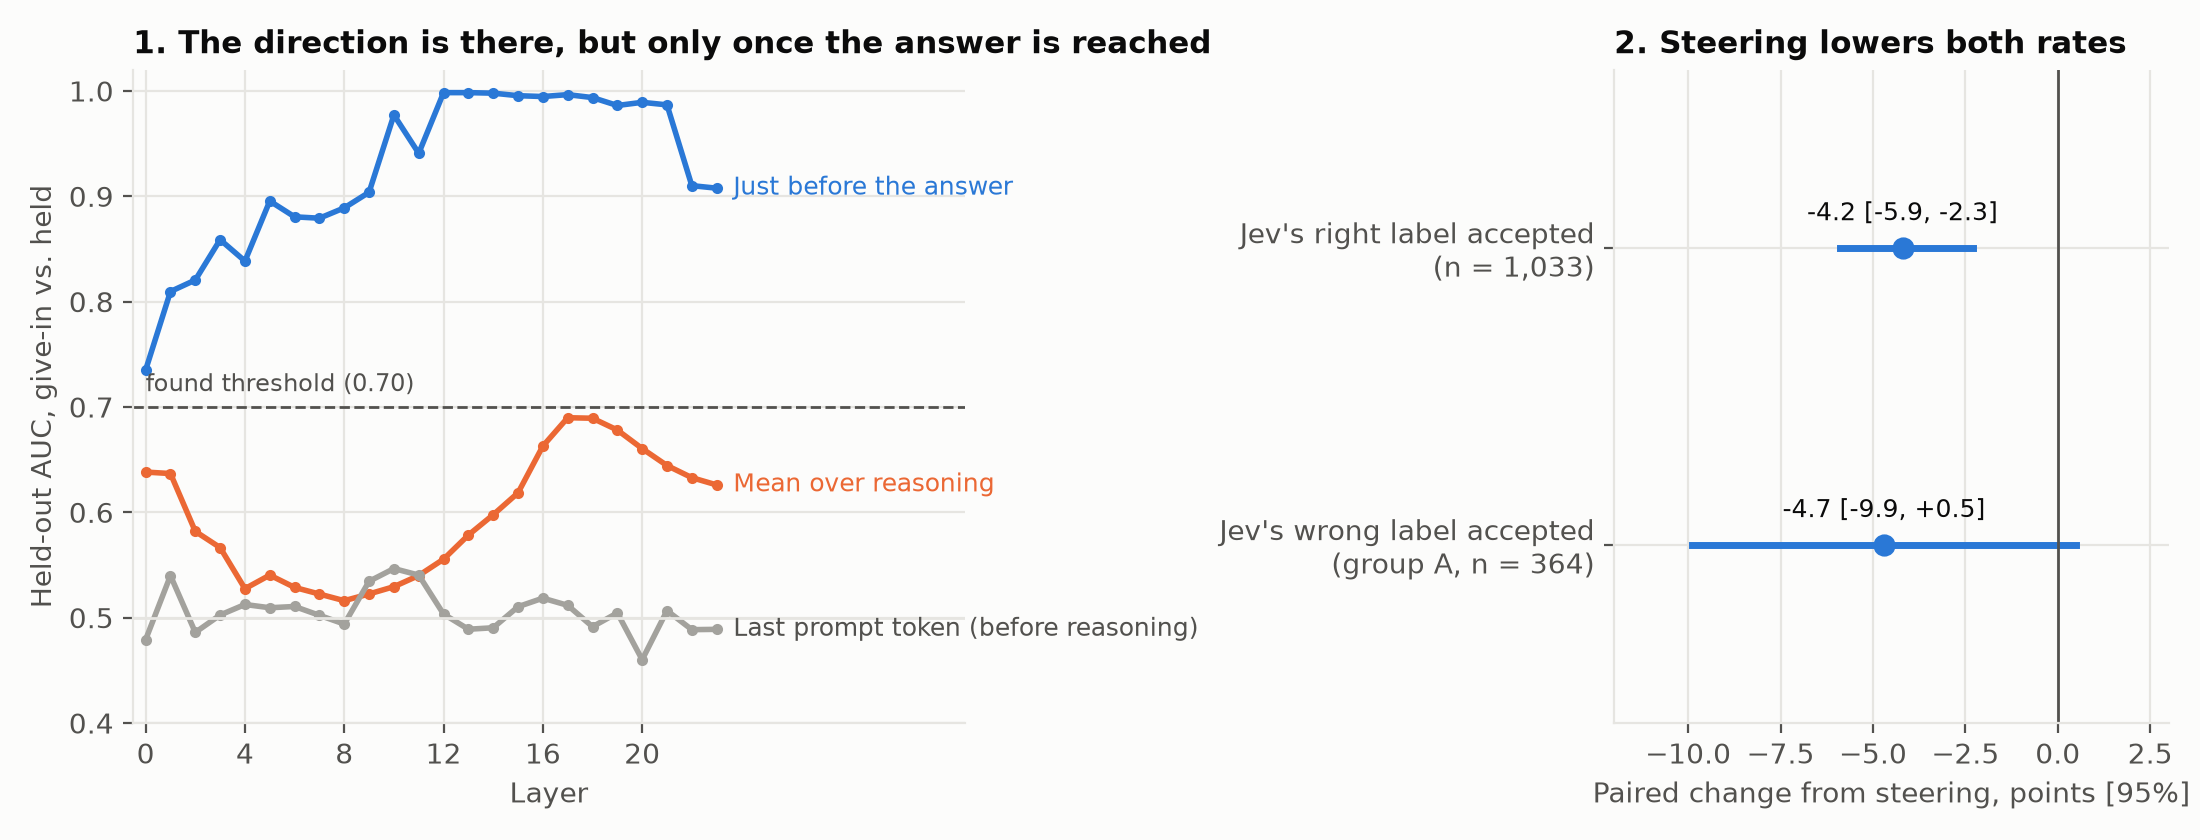
\includegraphics[width=\textwidth]{figures/e110_found_not_causal.png}
\caption{E.110. Left: held-out AUC of the give-in direction per layer at three positions (98 held-out items, 352 traces). Right: paired change from steering at $\alpha = 0.5$, layers 11--13, on the test set.}
\label{fig:e110}
\end{figure}

\begin{table}[H]
\centering
\small
\begin{tabularx}{\textwidth}{@{}lXX@{}}
\toprule
& Jev's wrong label accepted (group A) & Jev's right label accepted \\
\midrule
\multicolumn{3}{@{}l}{\emph{$\alpha$ selection (held-out training items)}} \\
$\alpha = 0$ & 59\% (77/131) & 95\% (142/150) \\
$\alpha = 0.5$ & 51\% (67/131) & 87\% (131/150) \\
$\alpha = 1$ & 50\% (65/130) & 91\% (137/150) \\
$\alpha = 2$ & 44\% (55/124) & 79\% (115/145) \\
$\alpha = 4$ & 38\% (21/55) & 42\% (22/53) \\
\midrule
\multicolumn{3}{@{}l}{\emph{Test set}} \\
Unsteered (transformers) & 27\% (100/364) & 92\% (954/1033) \\
Steered, $\alpha = 0.5$ & 23\% (83/364) & 88\% (912/1034) \\
Base on vLLM (E.106, reference) & 25\% (91/364) & 90\% (930/1034) \\
Paired change, unsteered $\to$ steered & $-4.7$ [$-9.9$, $+0.5$] & $-4.2$ [$-5.9$, $-2.3$] \\
\bottomrule
\end{tabularx}
\caption{E.110: $\alpha$ selection and measurement 2. At $\alpha = 4$, 108 of 207 reviews ran to the 4{,}352-token limit and did not parse.}
\label{tab:e110}
\end{table}

\emph{Measurement 1: found.} Just before the answer, the direction separates give-in from held traces almost perfectly: held-out AUC 0.998 at layer 12, and above 0.97 from layer 10 on. At the last prompt token it is at chance at every layer (0.46--0.55), and over the reasoning it reaches at most 0.69.

\emph{$\alpha$:} no $\alpha$ kept accept-when-right within 2 points, so by the rule the smallest, $\alpha = 0.5$, was frozen and flagged as not admissible. At $\alpha = 4$ the model breaks down.

\emph{Measurement 2: not causal.} Steering lowers acceptance of Jev's wrong labels on group A by 4.7 points, with an interval that crosses 0, and lowers acceptance of Jev's right labels by 4.2 points, more than the 2 allowed. The unsteered transformers pass matches the base's vLLM run within noise, so the replay is faithful.

\paragraph{Interpretation.}
The give-in signal exists, but only once the reasoning has reached its answer: nothing before the reasoning predicts it. Just before the answer, the direction mostly encodes which label is about to be written. Removing it does not remove deference specifically. It makes the reviewer agree with \emph{any} proposal a little less, lowering wrong and right acceptance by about the same amount, the same trade the prompt variants of E.103 and the training of E.106--E.108 made. Deference in this reviewer is decided item by item inside the reasoning, not by a separable switch. Caveats: gpt-oss-20b is a mixture-of-experts model, the traces were generated on Bedrock and replayed on our stack, the controls were cut short, and only one $\alpha$ was tested on the test set. Measurement 3, whether E.108's training changed the direction, was not run.

\paragraph{How it changed what came next.}
With E.108 and E.110 both null, we treat post-training as closed for this cascade (Section~\ref{sec:conclusion}). The next track was prompt engineering (Section~\ref{sec:prompteng}), which needs no GPU.

\section{Prompt engineering: a separate track}\label{sec:prompteng}

With post-training closed, we asked whether a different prompt could change what the reviewer catches with no training at all. Prompt changes were made a separate track on 2026-11-21 (\texttt{research\_docs/16\_prompt\_engineering.md}), kept apart so that no prompt is ever mixed into a training result. The standard reviewer prompt stays frozen, and a test pins it byte for byte. Every prompt here is a labelled arm, compared with the standard prompt on the same items. E.103 had already tested prompts about \emph{how much to trust Jev} (Section~\ref{sec:e103}). This track tested prompts about \emph{how to apply the policy}, aimed at the one specific failure round~2 found: the reviewer over-flags benign WildGuard items that a stronger reader gets right from the text (step~0, E.112). The track was WildGuard only. Civil Comments keeps the standard prompt, because many of its gold labels are doubtful (E.105, E.112), and tuning a prompt to them would chase label noise. It was planned in three steps:
\begin{itemize}[leftmargin=*,itemsep=2pt]
  \item E.115: a free audit of our policy text;
  \item E.116: a development screen on training pools only, with a selection rule fixed beforehand;
  \item E.117: one confirmatory test of the chosen arm on E.102's frozen test plan.
\end{itemize}
No prompt wording was written from test items.

\subsection{E.115: WildGuard policy-text audit}\label{sec:e115}

\paragraph{What we ran and why.}
Jev and the reviewer get the same policy text, a paraphrase of WildGuard's risk taxonomy (Section~\ref{sec:system}). If that paraphrase left out distinctions WildGuard's annotators were given, part of the over-flagging would be a measurement problem: both models would have been given a vaguer rule than the one the gold labels were made under. E.115 compares the two line by line, and its output is the clarification paragraph E.116's \texttt{clarify} arm uses.

\paragraph{Setup and how we ran it.}
\begin{itemize}[leftmargin=*]
  \item \textbf{Sources:} the WildGuard paper (Han et al., 2024): its taxonomy (Appendix A.6), how its labels were made (Section 3.2, Appendix D.2) and the annotators' instructions (Appendix E, Figures 3--9).
  \item \textbf{Transcription:} the instructions are published only as screenshots. A subagent transcribed them on 2026-11-23, and we checked the transcription against the figures; it needed no corrections.
  \item \textbf{No items read:} no WildGuard item, training or test, was read for the audit.
  \item \textbf{Cost:} \$0.
\end{itemize}

\paragraph{Results.}
Table~\ref{tab:e115} gives the main rows of the audit; the full table has 14 rows.

\begin{table}[H]
\centering
\small
\begin{tabularx}{\textwidth}{@{}Xp{3.4cm}X@{}}
\toprule
Annotator rule & In our policy text? & What the \texttt{clarify} arm adds \\
\midrule
The four categories and 13 subcategories & Yes & -- \\
``Harmful by common sense'' even if no category fits & No & This rule, stated \\
Judge the \emph{core request}, ``directly or implicitly'' & Partly & ``Judge the core request \ldots'' \\
Adversarial framing hides the core request & Yes (role-play, fiction, ignore-rules) & Adds a stated research purpose and coded words \\
Harmful-sounding words in a benign request & Yes & Restated, without examples \\
Science or history of a dangerous thing, no instructions & Partly & Stated \\
Quoting or critiquing harmful content & No; the guidelines don't address it either & Nothing (no guideline text) \\
A response is judged on its own content & Yes & Restated \\
Redirecting and selective refusals are not harmful & Partly & Stated \\
Harm after a refusal, behind a disclaimer or in a story & Partly & Stated \\
\bottomrule
\end{tabularx}
\caption{E.115: main rows of the policy-text audit. Full table and transcription: \texttt{research\_analyses/E115}. A list of benign prompt types taken from WildGuard's data generation was drafted for row 5 and cut on 2026-11-23: annotators never saw it, and it nudged toward ``unharmful''.}
\label{tab:e115}
\end{table}

\begin{itemize}[leftmargin=*]
  \item \textbf{No real mismatch.} Our text covers the distinctions the annotators were given. Its largest gap is the missing ``harmful by common sense'' rule, which pushes toward \emph{harmful}, so it cannot explain over-flagging.
  \item \textbf{None of step~0's three over-flagging triggers is a rule the annotators had and we lack.} A harm keyword in a harmless setting and judging a response by its request are covered by both texts. A stereotype quoted in order to criticize it is covered by neither: annotators decided those by their own judgment.
  \item \textbf{The labels matter more than the wording.} WildGuardTest's annotators agreed only moderately (Fleiss $\kappa$ 0.55 on prompts, 0.50 on responses). The training pools' labels are GPT-4's: they agree with human votes on 92\% of prompts and 82\% of responses, and GPT-4's labelling prompt makes every refusal unharmful by construction.
\end{itemize}

\paragraph{How it changed what came next.}
The over-flagging is not explained by a vaguer rule, so we gave the \texttt{clarify} arm a lower prior than planned. Because the label rules differ between training and test pools, development gains on responses are the least likely to carry over to E.117.

\subsection{E.116: Prompt-engineering development screen}\label{sec:e116}

\paragraph{What we ran and why.}
E.116 screens four prompt arms against the standard prompt on development items, and picks at most one for the confirmatory test by a rule fixed beforehand. Only one prompt may ever reach the test set.

\paragraph{Connection to earlier work.}
The items are E.104's training mix on the WildGuard training pools, so no Jev calls were needed and the test pools were not touched. The reviewer, its settings and the review format are E.102's and E.103's. The \texttt{clarify} text comes from E.115.

\paragraph{Setup.}
\begin{itemize}[leftmargin=*]
  \item \textbf{Items:} 1{,}268 items:
  \begin{itemize}[itemsep=1pt]
    \item all 668 of Jev's WildGuard training mistakes: 490 over-flagged (gold unharmful, Jev said harmful) and 178 let through (gold harmful, Jev said unharmful);
    \item 300 items Jev got right per pool, chosen by hash.
  \end{itemize}
  \item \textbf{Reviewer:} gpt-oss-20b, one review per item per arm, with Jev's label shown.
  \item \textbf{Arms:}
  \begin{itemize}[itemsep=1pt]
    \item \texttt{standard}: re-run on these items, so every comparison is paired;
    \item \texttt{clarify}: E.115's paragraph appended to the reviewer's policy only, so Jev's policy is unchanged;
    \item \texttt{grounded}: before calling an item harmful, name the category and quote the content; if nothing can be quoted, it is unharmful;
    \item \texttt{examples}: six hand-written worked examples per task, three benign items with harm vocabulary and three disguised harmful ones, drafted from the guidelines and edited and approved by the team; no example was written from a test item;
    \item \texttt{clarify+grounded}: both.
  \end{itemize}
  \item \textbf{Selection rule:} an arm is admissible if it:
  \begin{itemize}[itemsep=1pt]
    \item keeps accept-when-right within 2 points of \texttt{standard};
    \item lowers override of Jev's let-through items by at most 3 points;
    \item parses at least 95\% of replies.
  \end{itemize}
  Among admissible arms, the one with the largest gain in override of Jev's wrong labels goes to E.117, but only if that gain is at least 5 points with its 95\% interval above 0. Otherwise nothing does, and that is the track's result.
\end{itemize}

\paragraph{How we ran it.}
Run \texttt{e116-v1-2026-11-23} on Bedrock on 2026-11-24 (UTC). It made 6{,}340 reviews in 33 minutes, with no errors and one reply that did not parse. It cost \$0.58 against a \$2 cap and a projection of \$0.50--0.70.

\paragraph{Results.}
Figure~\ref{fig:e116} and Table~\ref{tab:e116} give the paired changes, with both WildGuard pools pooled.

\begin{figure}[H]
\centering
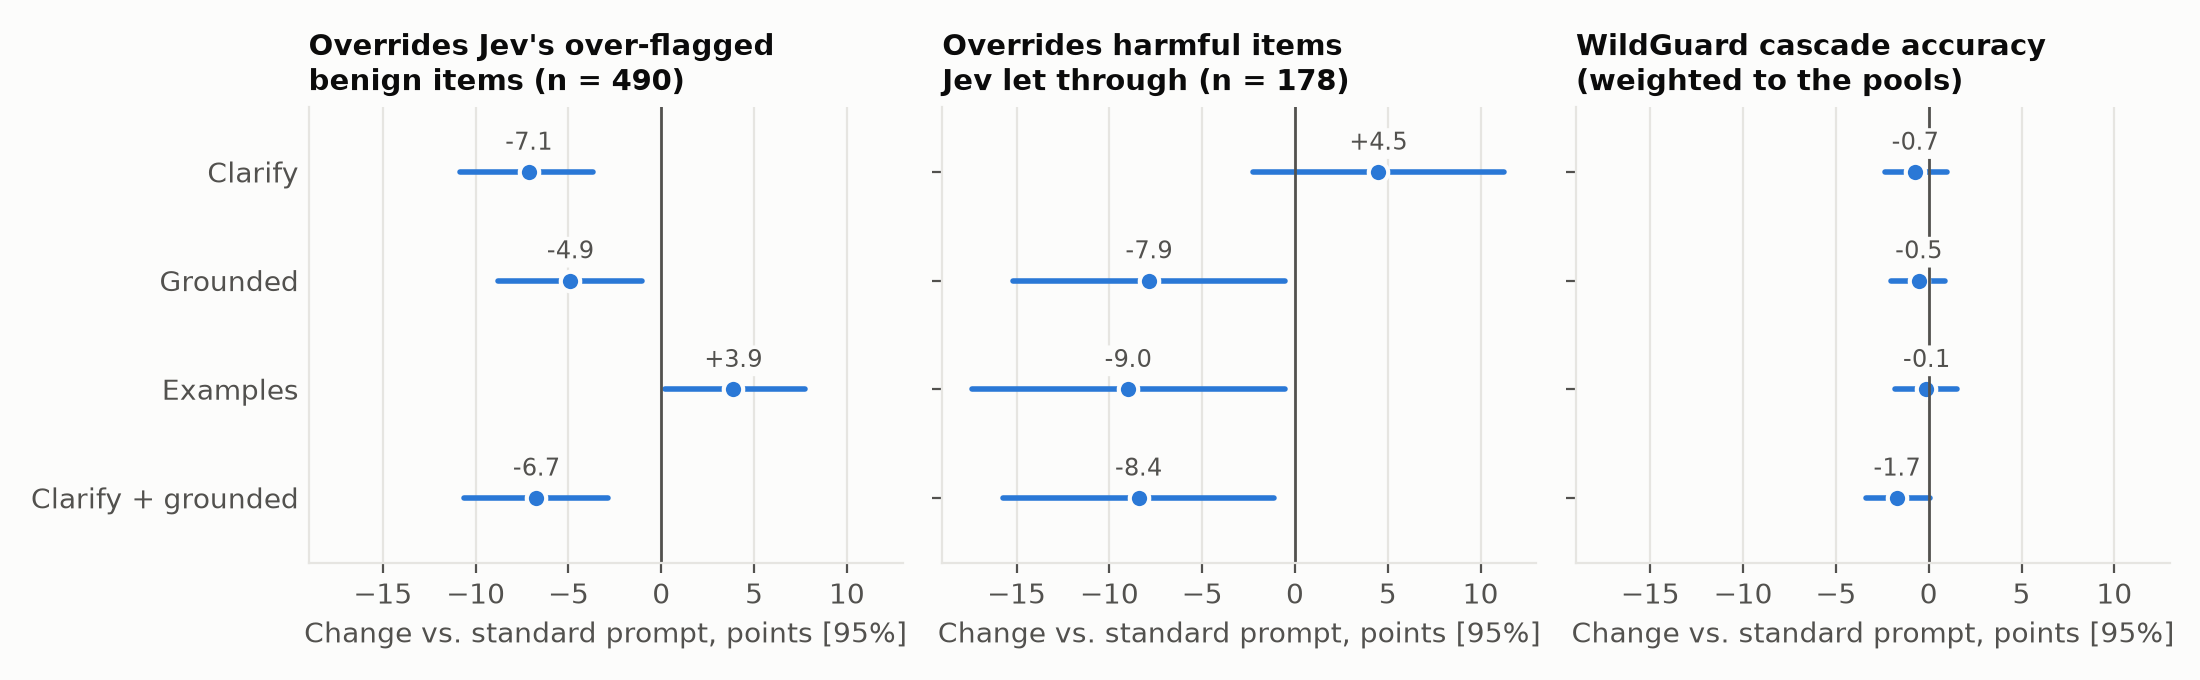
\includegraphics[width=\textwidth]{figures/e116_no_arm_helps.png}
\caption{E.116: each prompt arm's paired change against the standard prompt on WildGuard training items, with 95\% intervals. Left: Jev's over-flagged benign items overridden. Middle: harmful items Jev let through overridden. Right: cascade accuracy, weighted back to the pools.}
\label{fig:e116}
\end{figure}

\begin{table}[H]
\centering
\footnotesize
\begin{tabularx}{\textwidth}{@{}p{2.5cm}XXXXX@{}}
\toprule
Arm & Override Jev's wrong & Over-flagged & Let through & Accept Jev's right & Cascade accuracy \\
\midrule
\texttt{standard} (level) & 34\% (229/668) & 27\% (134/490) & 53\% (95/178) & 95\% (570/600) & 91.0\% \\
\texttt{clarify} & $-4.0$ [$-7.3$, $-0.8$] & $-7.1$ [$-10.8$, $-3.7$] & $+4.5$ [$-2.2$, $+11.2$] & $-0.5$ [$-2.3$, $+1.3$] & $-0.7$ [$-2.3$, $+1.0$] \\
\texttt{grounded} & $-5.7$ [$-9.0$, $-2.5$] & $-4.9$ [$-8.8$, $-1.0$] & $-7.9$ [$-15.2$, $-0.6$] & $-0.2$ [$-1.8$, $+1.3$] & $-0.5$ [$-2.1$, $+0.9$] \\
\texttt{examples} & $+0.4$ [$-3.3$, $+4.0$] & $+3.9$ [$+0.2$, $+7.8$] & $-9.0$ [$-17.4$, $-0.6$] & $-0.2$ [$-2.0$, $+1.7$] & $-0.1$ [$-1.8$, $+1.5$] \\
\texttt{clarify+}\linebreak\texttt{grounded} & $-7.2$ [$-10.6$, $-3.7$] & $-6.7$ [$-10.6$, $-2.9$] & $-8.4$ [$-15.7$, $-1.1$] & $-1.3$ [$-3.0$, $+0.5$] & $-1.7$ [$-3.4$, $+0.1$] \\
\bottomrule
\end{tabularx}
\caption{E.116: rates under the standard prompt, and each arm's paired change against it in points [95\% interval], WildGuard pooled. Cascade accuracy is weighted back to the pools. Every arm parsed at least 99.9\% of replies. Harmful content let through by the cascade was 3.8\% under \texttt{standard}; it rose by $+1.2$ [$-0.3$, $+2.9$] points under \texttt{examples}, and by $+3.2$ [$+1.1$, $+5.9$] on responses alone.}
\label{tab:e116}
\end{table}

\begin{itemize}[leftmargin=*]
  \item \textbf{No arm catches more of Jev's mistakes.} Three arms catch fewer: \texttt{clarify} $-4.0$, \texttt{grounded} $-5.7$ and both together $-7.2$, all with intervals below 0. \texttt{examples} is flat at $+0.4$.
  \item \textbf{The clarifications made over-flagging worse.} Under \texttt{clarify} and \texttt{grounded}, the reviewer overrode fewer of Jev's over-flagged benign items: $-7.1$ and $-4.9$ points.
  \item \textbf{Worked examples traded one error for the other.} They rescued a few over-flagged items ($+3.9$), but the reviewer overrode fewer of the harmful items Jev let through ($-9.0$).
  \item \textbf{Cascade accuracy didn't move.} Every arm is within 1.7 points of the standard prompt, with every interval crossing or touching 0.
  \item \textbf{Selection:} only \texttt{clarify} is admissible, and its gain is negative. \textbf{Nothing goes to E.117.}
\end{itemize}

\paragraph{Interpretation.}
Prompting the reviewer on how to apply the policy fails the same way prompting it on how much to trust Jev did (E.103). Spelling out the hidden-request rule and the ``harmful by common sense'' rule, or asking the reviewer to name a risk category, seems to push it toward calling items harmful, and asking it to find a category apparently lets it find one. Worked examples pushed the other way, toward ``unharmful'', on right and wrong items alike. As with post-training (E.106--E.110), what moves is the reviewer's overall lean toward accepting or rejecting a label, not which items it gets right.

Caveats:
\begin{itemize}[leftmargin=*,itemsep=2pt]
  \item The development labels are GPT-4's, not human, so a prompt that fails here could still help on human labels. The rule lets only one arm be tested on the test set, and none qualified.
  \item Each arm had one review per item.
  \item The guard checks are on point estimates.
  \item Exploratory, not a claim: on the prompt pool alone, \texttt{examples} raised override of Jev's wrong labels by $+4.8$ [$0.0$, $+9.7$], but on the response pool it lowered it by $5.1$ and raised harmful content let through.
\end{itemize}

\paragraph{How it changed what came next.}
By the plan's rule, E.117 does not run and the prompt-engineering track closes with a negative result. E.118, which would have combined a prompt with a trained reviewer, needed both a working prompt and a working training method, and has neither. One question was left: whether all of this is a limit of the small reviewer, which a stronger model would remove (Section~\ref{sec:e119}).

\section{A capability check: a stronger reviewer}\label{sec:capability}

\subsection{E.119: Does a stronger reviewer fix the cascade?}\label{sec:e119}

\paragraph{What we ran and why.}
Every intervention on gpt-oss-20b, whether prompts, five training methods or steering, moved only its overall lean toward agreeing or disagreeing. E.119 asks whether that is a limit of the 20b's capability, which a stronger reviewer would remove, or a property of the cascade itself. It is one cheap check, run before closing the project's main question.

\paragraph{Connection to earlier work.}
E.119 reuses E.102's design and frozen test plan unchanged (Section~\ref{sec:e102}): the same items, Jev labels, matched random wrong labels, random subsample, prompt and settings. Only the reviewer changes, from gpt-oss-20b to gpt-oss-120b (about $6\times$ larger, same family, medium reasoning effort, flex tier). No Jev calls were needed. E.112 had already screened gpt-oss-120b at high effort as a \emph{teacher} on training pools (Section~\ref{sec:e112}); here it is the reviewer, on the test plan.

\paragraph{Setup.}
\begin{itemize}[leftmargin=*]
  \item \textbf{Calls:} each reviewed item alone five times, plus one review of each proposal: 1{,}058 of Jev's wrong labels, 1{,}058 matched random wrong labels, and 1{,}200 correct labels on the random subsample (400 per pool).
  \item \textbf{Decision rule, fixed before the run} (\texttt{configs/experiments/e119.yaml}): a stronger reviewer fixes the cascade if the 120b cascade beats Jev alone on the pooled random subsample, paired, with the 95\% interval above 0.
  \item \textbf{Check before launch:} the comparison code, run with the 20b against itself, reproduces E.102 (the 20b cascade is 1.6 points below Jev on these 1{,}200 items).
\end{itemize}

\paragraph{How we ran it.}
Run \texttt{e119-v1-2026-11-24} on Bedrock on 2026-11-24 (UTC). It made 17{,}361 calls in 50 minutes with no errors, and cost \$1.70 against a \$5 cap and a projection of \$2.26. E.102's own analysis then ran on the new reviews unchanged, alongside a paired comparison of the two reviewers.

\paragraph{Results.}
Table~\ref{tab:e119-acc} gives accuracy on the random subsample and Table~\ref{tab:e119-wrong} the overrides of Jev's mistakes, both paired on the same items.

\begin{table}[H]
\centering
\footnotesize
\begin{tabularx}{\textwidth}{@{}>{\raggedright\arraybackslash}p{4.4cm}>{\raggedright\arraybackslash}X>{\raggedright\arraybackslash}X>{\raggedright\arraybackslash}X>{\raggedright\arraybackslash}X@{}}
\toprule
 & Civil Comments & WildGuard prompts & WildGuard responses & Pooled \\
\midrule
Jev alone & 76\% & 90\% & 92\% & 86\% \\
20b alone & 75\% & 90\% & 90\% & 85\% \\
120b alone & 79\% & 89\% & 90\% & 86\% \\
20b cascade & 77\% & 88\% & 88\% & 85\% \\
120b cascade & 77\% & 88\% & 90\% & 85\% \\
\midrule
\textbf{120b cascade $-$ Jev} & $+1.0$ [$-2.8$, $+4.8$] & $-2.2$ [$-4.5$, $0.0$] & $-2.8$ [$-5.2$, $-0.5$] & $\mathbf{-1.3}$ [$-3.1$, $+0.3$] \\
120b cascade $-$ 20b cascade & $-0.5$ [$-4.2$, $+3.2$] & $-0.2$ [$-2.5$, $+2.0$] & $+1.5$ [$-1.2$, $+4.0$] & $+0.2$ [$-1.4$, $+1.9$] \\
120b alone $-$ 20b alone & $+4.0$ [$+0.5$, $+7.8$] & $-0.8$ [$-3.2$, $+1.8$] & $+0.2$ [$-2.2$, $+2.8$] & $+1.2$ [$-0.5$, $+2.8$] \\
\bottomrule
\end{tabularx}
\caption{E.119: accuracy on E.102's random subsample (400 items per pool, pooled with equal weight), paired on the same 1{,}200 items. A reviewer ``alone'' is the majority of its five samples. Differences are in points [95\% paired bootstrap interval]. The bold row is the decision rule.}
\label{tab:e119-acc}
\end{table}

\begin{table}[H]
\centering
\footnotesize
\begin{tabularx}{\textwidth}{@{}>{\raggedright\arraybackslash}p{3.6cm}p{1.0cm}>{\raggedright\arraybackslash}X>{\raggedright\arraybackslash}X>{\raggedright\arraybackslash}X@{}}
\toprule
20b's record alone (5 samples) & Items & 20b overrides Jev & 120b overrides Jev & 120b right alone \\
\midrule
Never right (blind spots) & 434 & 6\% & 6\%\newline ($+0.5$ [$-2.8$, $+3.7$]) & 6\% \\
Sometimes right & 452 & 46\% & 34\% & 37\% \\
Always right & 172 & 92\% & 73\% & 78\% \\
\midrule
All of Jev's mistakes & 1{,}058 & 37\% & \textbf{29\%}\newline ($-8.2$ [$-11.2$, $-5.1$]) & 31\% \\
\bottomrule
\end{tabularx}
\caption{E.119: Jev's wrong labels on the test plan, grouped by the 20b's own record alone, pooled. The ``sometimes'' and ``always'' rows are selected on the 20b's record, so they favor the 20b by construction (regression to the mean); the fair comparisons are the ``all'' row, and the ``never'' row for shared blind spots.}
\label{tab:e119-wrong}
\end{table}

\begin{itemize}[leftmargin=*]
  \item \textbf{The rule fails.} The 120b cascade is $1.3$ points below Jev alone, pooled, with the interval crossing 0, and only $0.2$ points above the 20b cascade.
  \item \textbf{The blind spots are shared across model size.} On the 434 Jev mistakes the 20b never gets right alone, the 120b gets 6\% right alone and overrides Jev on 6\%, the same as the 20b. Its errors overlap with Jev's exactly as much as the 20b's do (phi 0.57 for both), and the two reviewers overlap with each other more (0.64).
  \item \textbf{The larger reviewer defers at least as much.} It overrides fewer of Jev's mistakes than the 20b (29\% against 37\%). At equal difficulty, E.102's measure gives $+6.1$ [$+2.2$, $+10.2$] points over all wrong proposals, $+9.6$ [$+3.8$, $+17.4$] on items it gets right alone, and $+8.0$ [$+3.8$, $+13.0$] on items it gets right in all five samples, against the 20b's $+7.8$, $+7.0$ and $+5.4$.
  \item \textbf{Its small solo gain does not reach the cascade.} Alone, the 120b is 4.0 points better than the 20b on Civil Comments, but in the cascade it gives that back by accepting more of Jev's labels.
\end{itemize}

\paragraph{Interpretation.}
A reviewer about as accurate as Jev, and wrong on the same items, can only tie or lose by reviewing Jev's labels, and a six-times-larger model of the same family is such a reviewer. The mistakes the cascade cannot fix are hard for this model family, not for a model of a particular size. With E.103--E.116, this answers the question the project kept returning to: the limit is not the 20b's capability. Prompts, training, steering and a larger reviewer all leave the cascade at or below Jev alone.

Caveats:
\begin{itemize}[leftmargin=*,itemsep=2pt]
  \item The larger model is the same family (gpt-oss), so it may share training data and blind spots with the 20b. A different family, or a reviewer clearly stronger than Jev alone, could behave differently. E.112 hints otherwise: as teachers, Mistral Large 3 and Qwen3-235B did not override more of Jev's mistakes than the 20b either, but that screen was small and on training pools.
  \item One size step, at medium reasoning effort; high effort was not tested as a reviewer.
  \item The pooled subsample weights the three pools equally, as in E.102 and E.103.
\end{itemize}

\paragraph{How it changed what came next.}
It closes the capability question for this model family, at one size step. The second batch (Section~\ref{sec:batch2}) then asked why every reviewer lands at or below Jev, and tested a reviewer from another family.

\section{Second batch: why no reviewer beats Jev (E.20--E.24)}\label{sec:batch2}

Every intervention in the first batch failed the same way: it moved the reviewer's overall lean toward accepting or overriding, and never changed \emph{which} items the reviewer gets right. The second batch (\texttt{research\_docs/17\_second\_batch.md}, numbered E.20--E.29 so the two batches cannot be confused) does two things with that. It explains the failure: a quantitative ceiling (E.20, E.20a), what a router and a reasoning monitor can still do (E.21), and what the shared blind spot is (E.24). And it tests the one route still open, a reviewer from another model family (E.22). A fifth experiment, re-labelling WildGuard's gold labels (E.23), needs hand labels and has not run. The rules of the first batch carried over: the standard reviewer prompt stayed frozen, no prompt or probe item was written from test items, every confirmatory test had a decision rule in its config before it ran, and labelling and reading were done by subagents separate from the agent designing the analysis.

\subsection{E.20: A correlation ceiling for the cascade}\label{sec:e20}

\paragraph{What we ran and why.}
E.20 asks whether a few numbers predict every cascade result we have, for any upstream model and any reviewer variant: how often each model is right alone, which items they get wrong together, and one or two deference parameters. It also asks what the most is that any reviewer could add. It was free, a re-analysis of saved runs.

\paragraph{Connection to earlier work.}
The tasks are binary and the reviewer is never told who proposed a label, so its review of ``label $L$ shown on item $i$'' is the same whichever upstream proposed $L$. Cascades with Llama 4 Maverick, Qwen3-32B, Nova Lite or a random-error upstream can therefore be computed from reviews already saved: E.102's reviews of correct, Jev and matched labels, and E.106's reviews of other upstreams' wrong labels (coverage 94--100\% of each upstream's items on E.102's subsample).

\paragraph{Setup.}
\begin{itemize}[leftmargin=*]
  \item \textbf{Ceiling.} The reviewer's alone vote share against the upstream's label is used as a detector of the upstream's mistakes. The ceiling is the best gain over the upstream alone of any threshold policy on that detector, with thresholds set separately for each proposed label. It is chosen on the same items, so it is an upper bound.
  \item \textbf{Deference model.} With $s$ the share of the reviewer's alone answers that are right on an item, the cascade is right with probability $s + (1-s)\,d_r$ when the right label is shown and $s\,(1-d_w)$ when the wrong one is. $d_w$ and $d_r$ are fitted per pool, by moments, on Jev $\to$ gpt-oss-20b only, then used to predict the other upstreams' cascades. The comparison is an \emph{independence} model that replaces $s$ with the pool's mean alone accuracy.
  \item \textbf{Rules, fixed before computing} (\texttt{configs/experiments/e20.yaml}): R1, every held-out cascade lies inside its prediction's 95\% interval and the item-level model beats the independence model; R2, no cascade with a five-sample reviewer is above its ceiling.
\end{itemize}

\paragraph{Results.}
Both rules pass. Table~\ref{tab:e20-pred} gives the predictions and Table~\ref{tab:e20-ceiling} the ceilings.

\begin{table}[H]
\centering
\footnotesize
\begin{tabularx}{\textwidth}{@{}>{\raggedright\arraybackslash}p{3.4cm}>{\raggedright\arraybackslash}p{2.0cm}>{\raggedright\arraybackslash}X>{\raggedright\arraybackslash}p{2.4cm}>{\raggedright\arraybackslash}p{2.4cm}@{}}
\toprule
Upstream $\to$ 20b & Upstream alone & Observed cascade [95\%] & Predicted, item-level & Predicted, independence \\
\midrule
Jev (fitted) & 86.2\% & 82.6\% [80.5, 84.6] & 83.0\% & 82.6\% \\
Llama 4 Maverick & 84.5\% & 83.0\% [80.9, 85.0] & 83.5\% & 81.4\% \\
Qwen3-32B & 85.7\% & 83.1\% [80.9, 85.1] & 83.3\% & 82.2\% \\
Nova Lite & 85.6\% & 83.1\% [81.1, 85.2] & 83.3\% & 81.9\% \\
Matched random & 86.2\% & 82.9\% [80.7, 84.9] & 83.0\% & 82.6\% \\
\bottomrule
\end{tabularx}
\caption{E.20, rule R1: cascades with gpt-oss-20b (vLLM, E.106) as reviewer on E.102's subsample, pooled. Mean absolute error over the four held-out cascades is 0.3 points for the item-level model and 1.0 for the independence model.}
\label{tab:e20-pred}
\end{table}

\begin{table}[H]
\centering
\footnotesize
\begin{tabularx}{\textwidth}{@{}Xp{3.4cm}p{3.6cm}@{}}
\toprule
Reviewer (5 alone answers) & Ceiling over Jev [95\%] & Observed cascade $-$ Jev [95\%] \\
\midrule
gpt-oss-20b, vLLM (E.106) & $+1.6$ [$+0.7$, $+3.2$] & $-3.6$ [$-5.6$, $-1.4$] \\
gpt-oss-20b, Bedrock (E.102) & $+2.2$ [$+1.3$, $+4.2$] & $-1.7$ [$-3.6$, $+0.2$] \\
E.103's four prompt protocols & $+2.2$ & $-1.9$ to $-2.3$ \\
gpt-oss-120b (E.119) & $+2.8$ [$+1.5$, $+4.5$] & $-1.3$ [$-3.1$, $+0.4$] \\
\bottomrule
\end{tabularx}
\caption{E.20, rule R2: the in-sample ceiling on what a threshold policy over the reviewer's own alone answers could add to Jev, against the observed cascade. Against weaker upstreams the ceiling is higher (Llama $\to$ 20b $+4.8$, Nova $\to$ 20b $+3.2$, random-error upstream $\to$ 20b $+2.9$), but those cascades are still below their upstreams (Llama $-1.4$, Nova $-2.5$).}
\label{tab:e20-ceiling}
\end{table}

\begin{figure}[H]
\centering
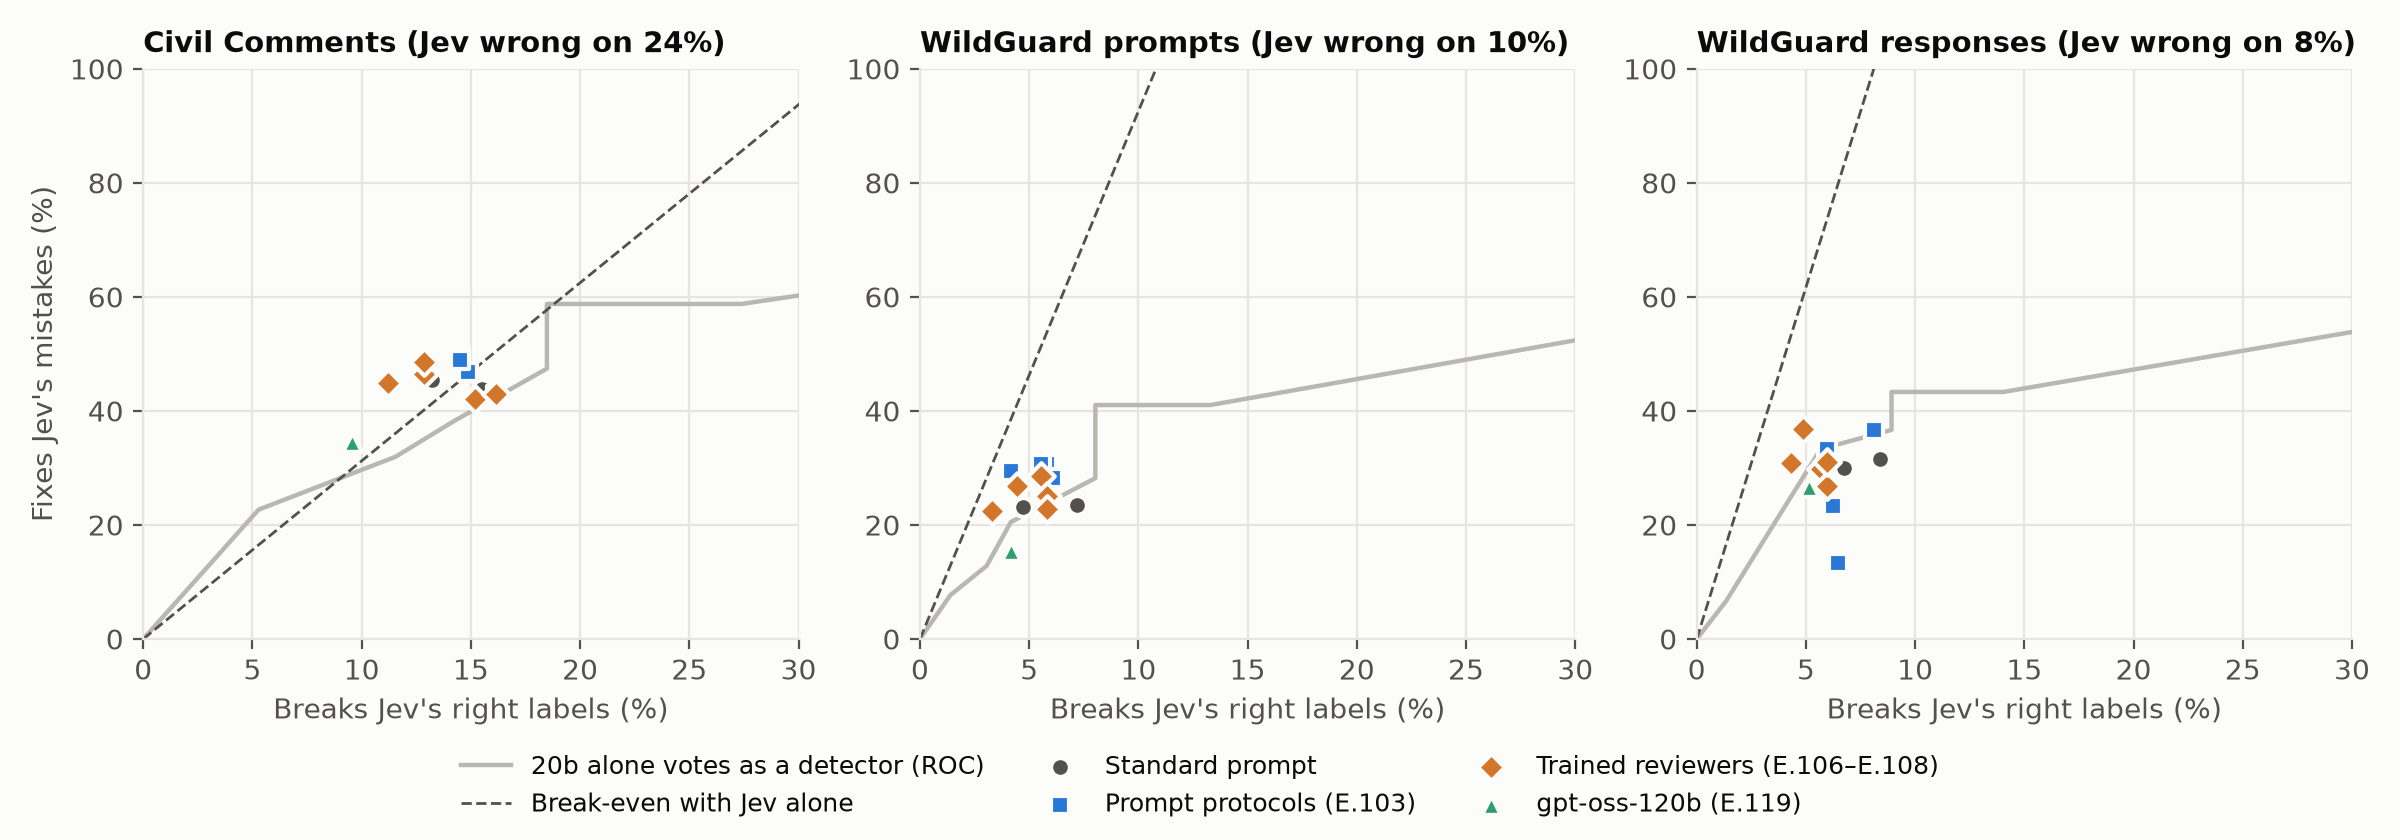
\includegraphics[width=0.85\textwidth]{figures/e20_frontier.png}
\caption{E.20: each reviewer variant's fix rate (share of Jev's mistakes overridden) against its break rate (share of Jev's right labels overridden), with Jev upstream. Above the dashed line the cascade would beat Jev alone. The grey curve is what thresholding the 20b's own alone answers can reach. On WildGuard every variant sits far below break-even, along the 20b's curve; on Civil Comments a few trained reviewers come near it ($+2.4$ at best, the DPO reviewer).}
\label{fig:e20-frontier}
\end{figure}

\begin{itemize}[leftmargin=*]
  \item \textbf{The reviewer re-decides; it barely defers.} The fitted deference parameters are 0 in every pool (unclipped estimates slightly negative), so the cascade review behaves like one more of its alone answers. The Bedrock 20b and the 120b show small positive deference ($d_w$ up to 0.24 and 0.40, largest on WildGuard, where the subsample has only 30--39 Jev mistakes).
  \item \textbf{The cascade's accuracy is set by the reviewer, not the upstream.} Every upstream's cascade with the 20b lands at 82.6--83.1\%, whatever that upstream's own accuracy (84.5--86.2\%).
  \item \textbf{Error overlap matters less than expected.} Across 57 pairs of upstream and reviewer, the ceiling correlates only weakly with phi (Spearman $-0.27$). With a random-error upstream (phi $\approx 0$) the 20b's ceiling is still only $+2.9$.
\end{itemize}

\paragraph{Interpretation.}
``Deference'' was the wrong frame for the cascade's \emph{accuracy}. E.102's deference ($+7$ points at equal difficulty) is real, but it compares Jev's wrong labels with random wrong labels. Measured against the reviewer's own alone answers, its one review adds almost nothing toward the proposed label. The cascade is right about as often as the reviewer alone, item by item, and a reviewer no more accurate than Jev pulls the cascade below Jev. The limiting arithmetic is the base rate: Jev is right 86\% of the time pooled and 90--92\% on WildGuard, so breaking 1\% of its right labels costs as much as fixing 6--10\% of its mistakes gains. Every intervention of the first batch moved the reviewer along a fixed curve of what its judgment can detect (Figure~\ref{fig:e20-frontier}); none moved the curve.

Caveats: the ceiling is in-sample and so optimistic. R1 is an easy test once deference is near 0, and the four upstreams have similar accuracy, so the independence model's error is only 1.0 point.

\paragraph{How it changed what came next.}
The ceiling suggested one cheap policy: override only when several alone answers agree, with a threshold per label. E.20a tested whether that survives out of sample.

\subsection{E.20a: Selective override, out of sample}\label{sec:e20a}

\paragraph{What we ran and why.}
E.20's $+1.6$ to $+2.8$ points were in-sample. E.20a chooses a selective-override policy on the training pools and tests it once on E.102's subsample. It was free.

\paragraph{Setup.}
For each pool and each label Jev proposed, one of three rules: never override; override if both of the reviewer's first two alone answers disagree with Jev (\emph{unanimous}); or override if at least one does (\emph{majority}). Rules were chosen on E.104's Jev decisions and E.105's alone tries (most training items have exactly 2 tries, hence $n = 2$), reweighted to Jev's real error rate in each direction. The rule, fixed before computing (\texttt{configs/experiments/e20a.yaml}), compares the chosen policy with Jev alone on the Bedrock 20b, paired.

\paragraph{Results.}
\begin{itemize}[leftmargin=*]
  \item \textbf{The chosen policy gains $-0.3$ points over Jev [$-1.8$, $+1.2$].} With all 5 alone answers it gains $+0.4$ [$-0.8$, $+1.6$]; on the vLLM 20b, $-0.2$ and $+0.4$. It stops the plain cascade's loss ($-1.7$ for the same reviewer) but adds nothing over Jev. It overrides 67, 15 and 4 of the 400 items per pool, a sixth to a hundredth as often as the plain cascade.
  \item \textbf{Even on training the best estimated gain in any direction is $+1.3$ points} (overriding Jev's ``harmful'' on WildGuard prompts).
  \item \textbf{The in-sample best rule on the test items gains $+1.2$ [$+0.3$, $+2.0$] but overrides in other directions.} On WildGuard prompts it overrides only Jev's ``unharmful''; training chose the opposite direction.
\end{itemize}

\paragraph{Interpretation.}
A careful override policy turns the cascade into a tie with Jev, as E.114's confidence routing did: a cost lever, not an accuracy lever. E.20's ceiling is mostly in-sample optimism. On WildGuard the training pools' labels (GPT-4's) and the test labels (human) point in opposite directions, which alone could explain the WildGuard part of the failure. That is the label question E.23 would answer.

\subsection{E.21: Routing to a person, and a deference monitor on the reasoning}\label{sec:e21}

\paragraph{What we ran and why.}
If the reviewer cannot correct Jev, it might still be useful for \emph{triage}: picking which items a person should check (Part~A, free). And E.110 found a ``give in'' direction inside the model; Part~B asks whether giving in is also readable in the reasoning text, which is the project's explainability question.

\paragraph{Setup.}
\begin{itemize}[leftmargin=*]
  \item \textbf{Part A.} A router sends the $k$\% of items with the highest risk score in each pool to a person, assumed always right, on E.102's subsample. Signals: Jev's confidence; the 20b's alone disagreement with Jev (5 answers); its cascade override (1 call); and a logistic regression combining them, fitted on the training pools only. Rule A: at a 10\% budget, the combined score catches more of Jev's mistakes than Jev's confidence, with the interval above 0.
  \item \textbf{Part B.} Reviews of Jev's labels are classed by outcome and the reviewer's alone majority: \emph{gave in} (accepted Jev's wrong label, right alone), \emph{held firm} (overrode it, right alone), \emph{genuine} (accepted it, never right alone) and \emph{correct accept} (accepted Jev's right label). Two monitors read the reasoning: a lexical one (TF-IDF on word 1--2-grams with logistic regression, trained on gave-in against correct-accept training traces from E.105), and a gpt-oss-120b judge that sees only the proposed label and the reasoning and scores 0--10 how much the decision rests on the label, with a prompt written from training traces only. Rule B: the monitor with the higher training AUC reaches test AUC $\ge 0.70$ (gave in against correct accept) with the interval's lower end above 0.60. Test traces are E.106's vLLM base run.
\end{itemize}

\paragraph{How we ran it.}
Part~A and the lexical monitor used saved runs. The judge ran as \texttt{e21-judge-v1-2026-11-24} on Bedrock: 2{,}024 calls (293 development, 1{,}731 test), 2 unparsed, \$0.21 against a \$1.50 cap, after a 12-call pilot.

\paragraph{Results.}
\begin{table}[H]
\centering
\footnotesize
\begin{tabular}{lrrr}
\toprule
Signal & 5\% sent & 10\% sent & 25\% sent \\
\midrule
Random & 4.0\% & 11.2\% & 26.0\% \\
Jev's confidence & 18.5\% & 30.8\% & 62.1\% \\
20b alone disagreement (5 calls) & 17.5\% & 29.5\% & 61.3\% \\
20b cascade override (1 call) & 18.8\% & 28.8\% & 63.0\% \\
Combined & 18.7\% & \textbf{35.2\%} & 63.9\% \\
Combined + lexical monitor (reported only) & 21.1\% & 34.1\% & 64.4\% \\
\bottomrule
\end{tabular}
\caption{E.21 Part A: share of Jev's mistakes caught when the riskiest $k$\% of items per pool go to a person (E.102's subsample, pools weighted equally). Rule A compares the bold cell with Jev's confidence: $+4.4$ points [$-1.7$, $+10.0$], fail.}
\label{tab:e21-route}
\end{table}

\begin{table}[H]
\centering
\footnotesize
\begin{tabular}{lccc}
\toprule
Monitor & Gave in vs.\ correct accept & Gave in vs.\ genuine & Gave in vs.\ held firm \\
\midrule
\textbf{Lexical} & \textbf{0.92} [0.89, 0.94] & 0.85 [0.80, 0.89] & 0.73 [0.68, 0.78] \\
Judge (gpt-oss-120b) & 0.41 [0.36, 0.46] & 0.47 [0.41, 0.52] & 0.81 [0.76, 0.86] \\
\bottomrule
\end{tabular}
\caption{E.21 Part B: test AUC of the two reasoning monitors. Test classes: 78 gave in, 286 held firm, 437 genuine, 930 correct accepts. Rule B (bold) passes. The lexical monitor had the higher training AUC (0.86 against the judge's 0.46 on development traces).}
\label{tab:e21-monitor}
\end{table}

\begin{itemize}[leftmargin=*]
  \item \textbf{Routing: the reviewer adds nothing clear over Jev's confidence.} In the combined model's training fit, Jev's confidence carries most of the weight.
  \item \textbf{Most of Jev's mistakes are silent.} In 55\% of Jev's 1{,}058 test mistakes, the reviewer's alone majority agrees with Jev and its cascade review accepts: 9\% of group A, 51\% of group B and 92\% of group C. The share is similar in every pool (53\%, 60\%, 59\%).
  \item \textbf{The lexical monitor reads giving in.} Within each proposed label it still separates gave in from correct accepts (0.89--0.94) and from genuine agreement (0.75--0.91), so it is not just reading the label word. Words pointing to giving in are unresolved hedges (\emph{but}, \emph{might be}, \emph{mild}, \emph{no direct}); words pointing to a correct accept are decisive conclusions (\emph{so verdict accept}, \emph{is insulting}).
  \item \textbf{The judge fails.} It separates accepting from overriding but rates correct accepts as \emph{more} label-dependent than giving in; it appears to read ``the automated label is correct, so accept'' as deference.
  \item \textbf{Giving in is rare,} 78 of the reviews of Jev's mistakes, so the monitor adds nothing as a routing signal (34.1\% against 35.2\%).
\end{itemize}

\paragraph{Interpretation.}
For the explainability question, this kind of deference \emph{is} visible in the explanation, as unresolved uncertainty, to a monitor trained on outcomes; an LLM judge asked to recognize deference in the words does not see it. It is the text-level counterpart of E.110's internal direction. But it is a small part of the problem. The mistakes that matter are the confident shared ones, which leave no trace in the cascade's disagreement, overrides or reasoning.

Caveats: the lexical monitor may partly read item difficulty, since gave-in items may be more borderline; gave in against held firm, which controls for that better, is weaker (0.73, and near chance within three of the four labels on 11--15 gave-in items each). Training traces came from Bedrock and test traces from vLLM (same weights). The judge prompt was one fixed attempt.

\subsection{E.22: A reviewer from another family, on WildGuard}\label{sec:e22}

\paragraph{What we ran and why.}
E.119 closed the capability question within gpt-oss; the open caveat was model family. In E.112's training-pool screen, Mistral Large 3 fixed far more of Jev's over-flagged WildGuard items than gpt-oss did (85 of 112 against 17). E.22 tests whether a Mistral reviewer beats Jev alone on WildGuard's \emph{test} items.

\paragraph{Setup.}
E.119's design on E.102's frozen plan, WildGuard prompts and responses only (400 + 400 in the subsample), with Mistral Large 3 as the reviewer: 3 alone samples per reviewed item plus one review of each proposal. Mistral is not a reasoning model, so the standard prompt gets E.112's instruction to write its reasoning before the JSON; nothing else changes. Rule, fixed before the run (\texttt{configs/experiments/e22.yaml}): Mistral cascade $-$ Jev $> 0$ on the pooled WildGuard subsample with the interval above 0, \emph{and} harmful items let through rise by no more than 1 point.

\paragraph{How we ran it.}
Run \texttt{e22-v1-2026-11-24} on Bedrock: 5{,}181 calls, 1 unparsed, \$4.19 against a \$6 cap, after a 162-call pilot (\$0.12). The run came in 35\% over the runner's \$3.11 projection: the pilot had measured a higher rate per call than the runner assumed (\$0.00077 against \$0.0006), and the projection was not updated.

\paragraph{Results.}
\begin{table}[H]
\centering
\footnotesize
\begin{tabularx}{\textwidth}{@{}>{\raggedright\arraybackslash}X>{\raggedright\arraybackslash}p{2.8cm}>{\raggedright\arraybackslash}p{2.8cm}>{\raggedright\arraybackslash}p{2.8cm}@{}}
\toprule
 & WildGuard prompts & WildGuard responses & Pooled \\
\midrule
Jev alone & 90\% & 92\% & 91\% \\
gpt-oss-20b alone & 90\% & 90\% & 90\% \\
Mistral alone & 85\% & 92\% & 89\% \\
20b cascade & 88\% & 88\% & 88\% \\
Mistral cascade & 84\% & 92\% & 88\% \\
\midrule
\textbf{Mistral cascade $-$ Jev} & $-6.5$ [$-10.0$, $-3.2$] & $-0.2$ [$-2.8$, $+2.2$] & $\mathbf{-3.4}$ [$-5.5$, $-1.1$] \\
Mistral cascade $-$ 20b cascade & $-4.5$ [$-8.5$, $-0.8$] & $+4.0$ [$+0.8$, $+7.5$] & $-0.2$ [$-2.6$, $+2.1$] \\
\bottomrule
\end{tabularx}
\caption{E.22: accuracy on the WildGuard subsample, paired on the same 800 items. Harmful items let through (share of all items): Jev 3.8\%, Mistral cascade 9.5\%, 20b cascade 3.5\%. Against the 120b cascade (E.119) on the same items: $-0.9$ [$-3.1$, $+1.5$].}
\label{tab:e22-acc}
\end{table}

\begin{table}[H]
\centering
\footnotesize
\begin{tabularx}{\textwidth}{@{}>{\raggedright\arraybackslash}X p{1.0cm} p{2.2cm} >{\raggedright\arraybackslash}p{3.2cm} p{2.2cm}@{}}
\toprule
20b's record alone & Items & 20b overrides Jev & Mistral overrides Jev & Mistral right alone \\
\midrule
Never right (shared blind spots) & 142 & 4\% & \textbf{37\%} ($+33$ [$+25$, $+42$]) & 42\% \\
Sometimes right & 131 & 44\% & 56\% & 57\% \\
Always right & 35 & 86\% & 46\% & 46\% \\
\midrule
All of Jev's WildGuard mistakes & 308 & 30\% & \textbf{46\%} ($+16$ [$+9$, $+23$]) & 49\% \\
\bottomrule
\end{tabularx}
\caption{E.22: Jev's wrong WildGuard labels, grouped by the 20b's record alone (as in Table~\ref{tab:e119-wrong}). Error overlap (phi): Jev--20b 0.64, Jev--Mistral 0.44, 20b--Mistral 0.32.}
\label{tab:e22-wrong}
\end{table}

\begin{itemize}[leftmargin=*]
  \item \textbf{The rule fails on both counts:} the cascade is 3.4 points below Jev, and harmful items let through rise by 5.8 points.
  \item \textbf{Mistral reaches the shared blind spots.} It overrides 37\% of the Jev mistakes the 20b never gets right, against the 20b's 4\%, and its errors overlap with Jev's much less.
  \item \textbf{But its errors run the other way.} Alone, it misses 30\% of harmful prompts (55 of 184) and 31\% of harmful responses (22 of 71), while over-flagging only 2\% of benign items; the 20b misses 8--10\% and over-flags 11--12\%.
  \item \textbf{Exploratory, not pre-registered:} letting Mistral overturn only Jev's ``harmful'' labels gives $-3.1$ [$-5.2$, $-1.1$], with 9.8\% let through. It un-flags real harm along with Jev's false alarms.
\end{itemize}

\paragraph{Interpretation.}
Lower error overlap is necessary but not enough: a reviewer must also be about as accurate as Jev in \emph{both} directions. Mistral trades Jev's over-flagging for letting harm through, mostly on prompts, where many of WildGuard's harmful test items are adversarial or indirect. This is E.20's arithmetic again, and the same trade as E.116's worked-examples prompt. Across sizes (E.119) and families (E.22), no reviewer we can afford beats Jev on WildGuard.

Caveats: written reasoning before the JSON rather than native reasoning, and no reasoning-mode model from another family was tried; 3 alone samples rather than 5; WildGuard only. WildGuardTest's human labels have only moderate annotator agreement ($\kappa$ 0.55 / 0.50, E.115), so some of Mistral's misses may be contestable labels (Section~\ref{sec:e23}).

\subsection{E.24: Minimal-pair probes of the shared blind spot}\label{sec:e24}

\paragraph{What we ran and why.}
Step~0 traced the shared over-flagging on WildGuard to a few kinds of trigger by reading items. Counting mistakes on natural items cannot separate a trigger from everything else in the text; controlled pairs can. E.24 asks whether those triggers \emph{cause} the errors, in Jev and gpt-oss alike, and whether a model from another family resists them.

\paragraph{Setup.}
\begin{itemize}[leftmargin=*]
  \item \textbf{Probe set} (\texttt{benchmarks/probes/minimal\_pairs\_v1}): 9 families of 20 triplets, 540 items. Each triplet is (a) a neutral benign item, (b) the same item with one trigger added, still benign, and (c) a minimal edit of (b) that is truly harmful. P1--P4 are prompt triggers (a harm word in a harmless setting; a stereotype quoted or critiqued; an education or safety question; dark fiction with no actionable request). R1--R2 are response triggers (a refusal; a response that discusses harm critically). C1--C2 are toxicity triggers (undirected mild profanity; a neutral identity mention). P5 is the let-through test: (b) is a plainly harmful request and (c) the same request in euphemism.
  \item \textbf{How the items were made.} Subagents wrote them from the task policies, WildGuard's published taxonomy and step~0's failure \emph{types} only, with no test item read. A script checked every item for character 8-gram overlap with every cascade pool, test and training. Two minimality reviews followed (the first led to 79 triplets being revised), and two blind labellers agreed with the intended label on all 540 items. Five triplets near the minimality line and 33 items a labeller marked unsure are flagged for a sensitivity check.
  \item \textbf{Models,} each deciding alone: Jev (jev-1.14.0) $\times 3$, gpt-oss-20b $\times 5$, gpt-oss-120b $\times 5$, Mistral Large 3 $\times 3$ (writing its reasoning first, as in E.22) and Qwen3-32B $\times 1$, plus one 20b cascade review of Jev's label per item. A model flags an item if most of its samples give the positive label.
  \item \textbf{Hypotheses, fixed before the run} (\texttt{configs/experiments/e24.yaml}): H1, the trigger raises the flag rate (P1--P4, b $-$ a) for Jev and the 20b; H2, Jev's and the 20b's trigger flags overlap (phi $> 0.3$), more than Jev's and Mistral's; H3, the cascade keeps Jev's trigger flags at least as often as it accepts Jev's natural mistakes; H4, euphemism lowers the flag rate on harmful requests (P5, c $-$ b).
\end{itemize}

\paragraph{How we ran it.}
Run \texttt{e24-v1-2026-11-24}: 9{,}720 calls (1{,}620 Jev, 8{,}100 Bedrock), 2 unparsed, \$1.22 (Bedrock \$1.18, TypeSafe \$0.04) against a projection of \$1.92, after a \$0.04 pilot. Intervals are paired bootstraps over triplets.

\paragraph{Results.}
\begin{itemize}[leftmargin=*]
  \item \textbf{H1 passes.} The trigger raises the flag rate by 16 points for Jev [$+8$, $+25$] and 32 for the 20b [$+21$, $+44$]; also 19 for the 120b, 20 for Qwen, and 1 for Mistral [0, $+4$]. Without the flagged triplets and items: Jev $+14$, 20b $+30$.
  \item \textbf{H2 passes.} On the trigger items, Jev's flags overlap with the 20b's (phi 0.41), the 120b's (0.48) and Qwen's (0.26), but not Mistral's ($-0.05$).
  \item \textbf{H3 fails.} Jev flagged only 14 trigger items, and the cascade kept 64\% of those flags (9 of 14) against 70\% on E.102's WildGuard prompts; $n = 14$ is too small to say much.
  \item \textbf{H4 fails.} Every model flags 95--100\% of the euphemistic versions.
\end{itemize}

\begin{table}[H]
\centering
\footnotesize
\begin{tabularx}{\textwidth}{@{}>{\raggedright\arraybackslash}Xcccccc@{}}
\toprule
Family (trigger) & Jev & 20b & 120b & Qwen3-32B & Mistral & 20b cascade \\
\midrule
P1 harm word, harmless setting & 5\% & 45\% & 25\% & 35\% & 5\% & 35\% \\
P2 stereotype quoted or critiqued & 5\% & 25\% & 5\% & 20\% & 0\% & 25\% \\
P3 education or safety question & 15\% & 20\% & 15\% & 0\% & 0\% & 20\% \\
P4 dark fiction, no actionable ask & \textbf{45\%} & \textbf{55\%} & 40\% & 25\% & 0\% & 35\% \\
R1 refusal of a harmful request & 0\% & 0\% & 0\% & 0\% & 0\% & 0\% \\
R2 response discusses harm critically & 5\% & 20\% & 5\% & 5\% & 0\% & 25\% \\
C1 undirected mild profanity & 0\% & 0\% & 5\% & 0\% & 0\% & 10\% \\
C2 neutral identity mention & 0\% & 0\% & 0\% & 0\% & 0\% & 0\% \\
\bottomrule
\end{tabularx}
\caption{E.24: flag rate on the benign trigger items (b), 20 per family. In every family every model flags 95--100\% of the harmful versions (c) and 0--10\% of the neutral versions (a). Full table: \texttt{research\_analyses/E24/data/report.md}.}
\label{tab:e24-families}
\end{table}

\paragraph{Interpretation.}
\begin{itemize}[leftmargin=*]
  \item \textbf{The shared blind spot has a cause we can name.} Benign prompts with dark fiction, harm vocabulary in a harmless setting, or a safety question get flagged as harmful, by Jev, both gpt-oss models and Qwen, on the \emph{same} items. This confirms step~0's reading by controlled edits rather than by reading.
  \item \textbf{The cascade makes it worse.} On P1--P4, Jev flags 18\% of the benign trigger items on average, the 20b alone 36\% and the 20b cascade 29\%; on R2 the cascade flags 25\% against Jev's 5\%. Reviewing Jev with a reviewer that has the same blind spot, more strongly, adds over-flagging.
  \item \textbf{Mistral does not have it,} which fits E.112's lead and E.22's blind-spot overrides. Its weakness on real WildGuard items is the opposite one: leniency on harmful items that are less plain than the probes' (c) versions.
  \item \textbf{The blind spot is specific.} Refusals, mild profanity and identity mentions trigger no model, and euphemism hides harm from none.
  \item \textbf{For explainability,} a cheap counterfactual probe set exposes \emph{which} input features drive a black box's mistakes and \emph{which other model} shares them, the kind of evidence the project's guiding question asks for.
\end{itemize}

Caveats: the probes are synthetic and short, so they show that the triggers \emph{can} cause errors, not how often each occurs in WildGuard's real mistakes. With 20 triplets per family the per-family intervals are wide; the hypotheses pool P1--P4. The labels are by construction, checked by subagent labellers, not people.

\subsection{E.23: Re-labelling WildGuard (not run)}\label{sec:e23}

E.23 would re-label WildGuard's gold labels to measure how much of ``the cascade loses to Jev'' and of the never-right group is label noise. Two blind subagent labellers would label the WildGuard subsample and every Jev-wrong WildGuard item; a person would label every item they disagree on plus an audit of 40 they agree on, an estimated 60--100 items. The rule, written in \texttt{research\_docs/17}: labels are part of the wall if, on consensus labels, the sign of 20b cascade $-$ Jev on the WildGuard subsample changes, or the never-right share of Jev's mistakes falls by at least a third. It needs hand labels and has not run.

What the saved runs say about its odds:
\begin{itemize}[leftmargin=*]
  \item \textbf{Only items where Jev and the cascade disagree can move the comparison.} On the 800 WildGuard subsample items, the 20b cascade fixes 17 of Jev's labels and breaks 42 (net $-25$). Each gold error on a broken item turns it into a fix (net $+2$). To change the sign, gold errors on broken items must outnumber those on fixed items by at least 13: about a third of the 42 breaks if the fixes are clean, about half of all 59 disagreements if errors fall evenly.
  \item \textbf{The 20b's breaks are the wrong kind for that.} 36 of its 42 breaks are benign-gold items the cascade over-flags, the type step~0 most often judged clear model mistakes. Among the benign-gold items step~0 read (25 of 30, a different population: items both models got wrong), it judged the gold label doubtful on 5, about 1 in 5, short of the third needed.
  \item \textbf{Mistral's breaks are the right kind.} 48 of its 52 breaks are harmful-gold items it let through, 40 of them adversarial prompts or responses; step~0 found every harmful-gold item it read doubtful or ambiguous (5 of 5). Its fixes are 23 benign-gold items. Mistral's cascade (net $-27$) would need gold errors on about 14 more breaks than fixes. That test is not in the rule.
  \item \textbf{The never-right leg turns on ambiguous items.} 142 of Jev's 308 WildGuard mistakes (46\%) are never right for the 20b; falling by a third means 31\%. Step~0 read 30 such items as 9 doubtful gold, 11 ambiguous and 10 clear model mistakes. Assuming Jev's other mistakes keep their labels: if only doubtful labels flip, the share falls to about 37\%, short; if ambiguous items are also dropped, it falls to about 22\%, a pass. The rule does not yet say how ambiguous items are treated.
\end{itemize}

\section{Summary of findings and current status}\label{sec:conclusion}

\paragraph{Phase 1 (explanation).} E0 showed that Jev is a stable, parseable decision function, with 24 customer-harming wrong decisions on \texttt{refund\_v1} (Section~\ref{sec:e0}). E1 Pilot~1 could not yet test faithfulness (RQ1): a simulator with no explanation already predicted Jev on 90\% of hidden variants, and the explanations restated the policy rather than Jev (Section~\ref{sec:e1p1}). Asked to explain Jev's three wrong past-window approvals, 10 of 12 explanations justified them, which bears on the stretch goal (SQ1). That rests on 3 cases and one LLM coder, so it is a lead, not a finding. The follow-up benchmark and judge were built but not run before the project moved to cascade deference.

\paragraph{Part 1: does the reviewer defer to Jev?} Yes, but mostly for a different reason than deference. The reviewer accepted 60\% of Jev's wrong labels on Civil Comments against 22\% of random wrong labels (E.102). Most of that gap comes from shared blind spots: Jev's mistakes fall on items the reviewer also gets wrong alone (E.101, E.102). At equal difficulty, deference was about $+7$ points pooled (95\% interval $+0.8$ to $+12.6$). It is real, but it is the smaller part of the problem. No cheap prompt change caught more of Jev's mistakes, and on items the reviewer never gets right alone it accepted 91--100\% of Jev's wrong labels under every prompt (E.103). In no experiment was the cascade more accurate than Jev alone beyond noise.

\paragraph{Part 2, round 1: post-training on the reviewer's own correct reasoning.} This did not help. SFT, with or without Jev's proposal in the prompt, failed all five pre-registered criteria, and switching to Jev's wrong label rose from 25\% to 32\% (E.106). DPO brought the main rates back near the base but caught no more of Jev's mistakes, and it also failed all five criteria (E.107). The common reason is how the data are made: self-training needs the reviewer to reach the right label at least sometimes, and the shared blind spots are by definition the items where it never does (E.105).

\paragraph{Part 2, round 2: cheap checks.} Round~2 split Jev's 1,058 test mistakes into groups A (34\%), B (21\%) and C (45\%) and built three training methods aimed at groups A and B (E.108--E.110). The four cheap checks that ran first found no cheap route to the mistakes the reviewer cannot fix alone:
\begin{itemize}[leftmargin=*,itemsep=2pt]
  \item \textbf{Step~0:} in one model reader's reading of 30 WildGuard group C items, 10 were clear model mistakes, exactly at the pre-registered threshold, and all 10 were over-flagging (Section~\ref{sec:step0}).
  \item \textbf{E.111:} Jev's own confidence ranks its mistakes well (test AUC 0.72 / 0.85 / 0.88), but flipping its least confident labels gains about 1 point or less (Section~\ref{sec:e111}).
  \item \textbf{E.112:} no affordable teacher passed the pre-registered screen. Each failed on override gain over gpt-oss-20b (Mistral Large 3 $+2.6$ points, interval $-8.2$ to $+14.2$; Qwen3-235B $-8.5$; gpt-oss-120b at high effort $-5.1$) (Section~\ref{sec:e112}).
  \item \textbf{E.113:} Claude could not be used as a teacher. Both agents were stopped by safeguards before any output, so there are no data (Section~\ref{sec:e113}).
\end{itemize}
One exploratory result, chosen after seeing the data, is kept separate from these: on WildGuard, Mistral fixed 85 of 112 benign items that Jev over-flagged, against 17 of 112 for gpt-oss-20b. It caught 8 of 28 harmful items Jev let through, against 11 of 28 for gpt-oss-20b. Its whole gain is in the over-flagging direction, and it has not been tested on fresh items.

\paragraph{Part 2, round 2: routing, training and steering.} Three more experiments ran on 2026-11-21 to 2026-11-23 (Section~\ref{sec:part2r2b}):
\begin{itemize}[leftmargin=*,itemsep=2pt]
  \item \textbf{E.114:} routing only Jev's least confident labels to the reviewer never beats Jev alone. Reviewing the lowest 10\% matches Jev ($-0.5$ points [$-1.6$, $+0.6$]) at a tenth of the reviewer calls, against $-3.5$ for reviewing everything. Even on those items the reviewer breaks more right labels than it fixes (Section~\ref{sec:e114}).
  \item \textbf{E.108:} consistency training and balanced-proposal SFT, aimed at groups A and B, fail R1--R3. Group A still gives in 24\% and 26\% of the time against the base's 25\%, and both cascades stay below Jev alone (Section~\ref{sec:e108}).
  \item \textbf{E.110:} a ``give in'' direction is found just before the answer (held-out AUC 0.998) but is at chance before the reasoning. Steering it out lowers acceptance of Jev's wrong labels ($-4.7$ points [$-9.9$, $+0.5$]) and right labels ($-4.2$ [$-5.9$, $-2.3$]) alike, so it is not causal (Section~\ref{sec:e110}).
\end{itemize}

\paragraph{Is post-training dead?} For this cascade and this goal, yes, with one untested exception. Five methods have now tried to make the reviewer catch more of Jev's mistakes: SFT with and without the proposal (E.106), DPO (E.107), consistency and balanced-proposal SFT (E.108), and activation steering (E.110). None caught more of Jev's mistakes. The trained models only learned to accept slightly more, and steering only learned to accept slightly less, of every label. E.110 suggests why. Giving in is not a separate switch: it is decided inside the reasoning, item by item, and the only global lever is a bias toward agreeing or disagreeing, which trades right labels accepted for wrong labels caught. Two further facts limit what any reviewer training could achieve here. First, almost half of Jev's mistakes are group C, where the reviewer is never right alone and self-training has nothing to learn from; distillation from a stronger teacher, the one route to those items, found no passing teacher (E.112, E.113). Second, even a perfect result on group A, the $+9$-point ceiling, was expected to leave the cascade below Jev alone (R6). The exception is GRPO (E.109), which rewards the gold label directly rather than imitating traces. It is the only mechanism not tried, and it is built and tested offline. We set it aside on 2026-11-23: it needs 2 $\times$ H100 for 6--15 hours (about \$80--200 at the observed price), and with group A unmoved by every other method and group C out of its reach, we judge its prior low. We would reopen post-training only with a reviewer whose solo accuracy is much closer to Jev's, or with a source of correct reasoning on group C.

\paragraph{Prompt engineering: a separate track.} With post-training closed, a separate track tested whether a different prompt could do what training could not, aimed at the reviewer's over-flagging of benign WildGuard items (Section~\ref{sec:prompteng}). The standard prompt stayed frozen, and no prompt was written from test items.
\begin{itemize}[leftmargin=*,itemsep=2pt]
  \item \textbf{E.115:} our WildGuard policy text covers the rules WildGuard's annotators were given. The over-flagging is not a measurement problem caused by a vaguer rule. The largest over-flagging trigger, a stereotype quoted in order to criticize it, is in neither text, and the annotators themselves agreed only moderately ($\kappa$ 0.55 / 0.50) (Section~\ref{sec:e115}).
  \item \textbf{E.116:} on 1{,}268 development items, no prompt arm caught more of Jev's mistakes.
  \begin{itemize}[itemsep=1pt]
    \item Policy clarifications and a ``name the category and quote it'' instruction caught fewer ($-4.0$ to $-7.2$ points) and made over-flagging worse.
    \item Worked examples rescued a few over-flagged items ($+3.9$) but let more harmful ones through ($-9.0$).
    \item Cascade accuracy stayed within 1.7 points under every arm.
  \end{itemize}
  No arm passed the selection rule, so the confirmatory test (E.117) and the prompt-and-training combination (E.118) did not run (Section~\ref{sec:e116}).
\end{itemize}
Together with E.103, prompts about how much to trust Jev and prompts about how to apply the policy have both failed. They move the reviewer's overall lean toward ``harmful'' or ``unharmful'', the same trade post-training made, without changing which items it gets right.

\paragraph{A stronger reviewer.} A last capability check asked whether a stronger reviewer would remove the limit (Section~\ref{sec:e119}). With gpt-oss-120b, about six times larger, as the reviewer on E.102's frozen test plan, the cascade was no more accurate than Jev alone ($-1.3$ points [$-3.1$, $+0.3$]) or than the gpt-oss-20b cascade ($+0.2$). On the 434 Jev mistakes the 20b never gets right alone, the 120b got 6\% right alone and overrode 6\%. Its errors overlapped with Jev's as much as the 20b's did (phi 0.57), and it overrode fewer of Jev's mistakes (29\% against 37\%). The shared blind spots hold across model size within this family.

\paragraph{Second batch: why no reviewer beats Jev.} Five experiments on 2026-11-24 explained the wall and tested the last open route (Section~\ref{sec:batch2}).
\begin{itemize}[leftmargin=*,itemsep=2pt]
  \item \textbf{E.20:} the reviewer re-decides rather than defers. Its cascade review behaves like one more of its alone answers (fitted deference $\approx 0$), so every upstream's cascade with gpt-oss-20b lands at 82.6--83.1\%, and a model of overlap and deference predicts four held-out cascades within 0.3 points. No threshold policy on the reviewer's own answers could add more than $+1.6$ to $+2.8$ points, even in-sample. The limit is the base rate: Jev is right 90--92\% of the time on WildGuard, so a reviewer must fix about ten of its mistakes for every right label it breaks.
  \item \textbf{E.20a:} chosen on the training pools, a selective-override policy ties Jev ($-0.3$ [$-1.8$, $+1.2$]); the ceiling was in-sample optimism.
  \item \textbf{E.21:} as a triage signal the reviewer adds nothing clear over Jev's confidence ($+4.4$ [$-1.7$, $+10.0$] at a 10\% budget), and 55\% of Jev's mistakes are silent: the reviewer agrees alone and accepts. When it does give in, a word-based monitor reads it in the reasoning (AUC 0.92 [0.89, 0.94]) as unresolved hedging; a gpt-oss-120b judge does not (0.41). Giving in is rare (78 reviews), so it matters little for accuracy.
  \item \textbf{E.22:} a Mistral Large 3 reviewer overrides 37\% of the WildGuard mistakes gpt-oss never gets right, against 4\%, but misses 30\% of harmful items alone. Its cascade is 3.4 points below Jev [$-5.5$, $-1.1$], with harmful items let through rising from 3.8\% to 9.5\%.
  \item \textbf{E.24:} on 180 minimal-pair triplets, dark fiction, harm words in a harmless setting and safety questions make benign prompts look harmful to Jev ($+16$ points), gpt-oss-20b ($+32$), gpt-oss-120b ($+19$) and Qwen3-32B ($+20$), on the same items (phi 0.41--0.48 with Jev). Mistral is immune ($+1$). The 20b cascade adds over-flagging on these items (29\% against Jev's 18\%).
\end{itemize}
The batch's answer is that a reviewer must be wrong on different items from Jev \emph{and} about as accurate in both directions. gpt-oss models fail the first condition, sharing Jev's triggers; Mistral fails the second, being lenient. For the explainability question, two results are positive: deference, when it happens, is visible in the reviewer's reasoning to a trained monitor (E.21), and a cheap counterfactual probe set names the input features behind the shared mistakes and which models share them (E.24).

\paragraph{What the project rules out and what it does not.} At this budget and on these samples, the project rules out: fixing Jev's mistakes by flipping on Jev's confidence (E.111); improving cascade accuracy by routing on Jev's confidence (E.114); reducing deference with SFT, DPO or consistency training on the reviewer's own traces (E.106--E.108); removing it with a single steering direction (E.110); catching more of Jev's WildGuard mistakes with prompts about how to apply the policy (E.116), as well as prompts about how much to trust Jev (E.103); fixing the cascade with a larger reviewer of the same family (E.119); a selective-override policy chosen out of sample (E.20a); routing to a person on the reviewer's signals beyond Jev's confidence (E.21); and, on WildGuard, a Mistral Large 3 reviewer (E.22). It also counts as a failed screen for distilling an affordable teacher across all pools (E.112). It does \emph{not} show that distillation cannot help: E.112's screen was small, and Mistral's interval cannot exclude the 10-point gain the rule asked for. It does not test GRPO, a reasoning-mode reviewer from another family or one clearly stronger than Jev, other tasks, or whether WildGuard's gold labels are part of the wall (E.23, which needs hand labels), and E.116's prompts were screened on GPT-4 labels, not human ones. All results carry the same scope limits: one reviewer, one upstream model and three moderation tasks.

\paragraph{Status.} No training, GPU work or live run is running, and every GPU machine and disk has been deleted. Both the post-training and the prompt-engineering tracks are closed, and the capability check (E.119) and the second batch (E.20--E.22, E.24) are done; E.23 waits on hand labels. Measured costs are Bedrock \$15.70 of \$50, the GCP API ledger \$0.20 and TypeSafe \$2.14 of \$5. GPU time is estimated from uptime at roughly \$13--22 for round~1, about \$57 for E.108 (including about \$32 idle) and about \$35 for E.110 (Table~\ref{tab:intro-budget}).

\end{document}
